%%%%%%%%%%%%%%%%%%%%%%%%%%%%% Thesis.tex %%%%%%%%%%%%%%%%%%%%%%%%%%%%%%%
%                                                                      %
%  ---------- Master of Science Dissertation template ----------       %
%                                                                      %
%  Template for the Master Thesis according to the regulations         %
%  published by the Academic Board (Direcção Académica) at IST.        %
%                                                                      %
%  For up-to-date guide, please refer to the official website          %
%  http://academica.tecnico.ulisboa.pt/alunos/dissertacao-de-mestrado/ %
%                                                                      %
%       Andre C. Marta                                                 %
%       Area Cientifica de Mecanica Aplicada e Aeroespacial            %
%       Departamento de Engenharia Mecanica                            %
%       Instituto Superior Tecnico                                     %
%       Av. Rovisco Pais                                               %
%       1049-001 Lisboa                                                %
%       Portugal                                                       %
%       Tel: +351 21 841 9469                                          %
%                        3469 (extension)                              %
%       Email: andre.marta@tecnico.ulisboa.pt                          %
%                                                                      %
%  Created:       Jan 20, 2011                                         %
%  Last Modified: Feb 19, 2018                                         %
%                                                                      %
%%%%%%%%%%%%%%%%%%%%%%%%%%%%%%%%%%%%%%%%%%%%%%%%%%%%%%%%%%%%%%%%%%%%%%%%
%  Revision history                                                    %
%  v1 - 2011/01/24 - original template                                 %
%  v2 - 2012/10/30 - new IST image and glossary support                %
%  v3 - 2013/12/10 - update according to 2012/13 official guide        %
%  v4 - 2014/02/28 - new default for bibliography style                %
%  v5 - 2014/05/07 - update according to 2013/14 official guide        %
%  v6 - 2015/07/02 - cover page format fixed,                          %
%                    contents page numbering fixed,                    %
%                    better language support,                          %
%                    enhanced examples of tables,                      %
%                    new option for appendix page numbering format,    %
%                    custom bibliography style                         %
%  v7 - 2018/02/19 - multiple citations compressed                     %
%%%%%%%%%%%%%%%%%%%%%%%%%%%%%%%%%%%%%%%%%%%%%%%%%%%%%%%%%%%%%%%%%%%%%%%%
%                                                                      %
% To generate the PDF file, type "make" at the terminal prompt.        %
%                                                                      %
% The IST template LaTeX package was created by the author             %
% and it can be downloaded from:                                       %
% https://fenix.ist.utl.pt/homepage/ist31052/                          %
%                                                                      %
% The external packages can be downloaded from                         %
% the Comprehensive TeX Archive Network at http://www.ctan.org/        %
%                                                                      %
% List of LaTex symbols:                                               %
% http://www.ctan.org/tex-archive/info/symbols/comprehensive/          %
%                                                                      %
% Help with LaTex can be found at                                      %
% http://www.giss.nasa.gov/tools/latex/ltx-2.html                      %
% http://en.wikibooks.org/wiki/LaTeX                                   %
%%%%%%%%%%%%%%%%%%%%%%%%%%%%%%%%%%%%%%%%%%%%%%%%%%%%%%%%%%%%%%%%%%%%%%%%

%%%%%%%%%%%%%%%%%%%%%%%%%%%%%%%%%%%%%%%%%%%%%%%%%%%%%%%%%%%%%%%%%%%%%%%%
%     Preamble                                                         %
%%%%%%%%%%%%%%%%%%%%%%%%%%%%%%%%%%%%%%%%%%%%%%%%%%%%%%%%%%%%%%%%%%%%%%%%

% ----------------------------------------------------------------------
%  Set the document class
% ----------------------------------------------------------------------
\documentclass[10pt,a4paper,twoside]{report}

\usepackage{float}
\usepackage{comment}

% ----------------------------------------------------------------------
% Define external packages, language, margins, fonts and new commands
% ----------------------------------------------------------------------
%%%%%%%%%%%%%%%%%%%%%%%%%%%%%%%%%%%%%%%%%%%%%%%%%%%%%%%%%%%%%%%%%%%%%%%%
%                                                                      %
%     File: Thesis_Preamble.tex                                        %
%     Tex Master: Thesis.tex                                           %
%                                                                      %
%     Author: Andre C. Marta                                           %
%     Last modified : 9 Apr 2015                                       %
%                                                                      %
%%%%%%%%%%%%%%%%%%%%%%%%%%%%%%%%%%%%%%%%%%%%%%%%%%%%%%%%%%%%%%%%%%%%%%%%

% ----------------------------------------------------------------------
% Define document language.
% ----------------------------------------------------------------------

% 'inputenc' package
%
% Accept different input encodings.
% http://www.ctan.org/tex-archive/macros/latex/base/
%
% > allows typing non-english text in LaTeX sources.
%
% ******************************* SELECT *******************************
%\usepackage[latin1]{inputenc} % <<<<< Windows
\usepackage[utf8]{inputenc}   % <<<<< Linux
% ******************************* SELECT *******************************


% 'babel' package
%
% Multilingual support for Plain TeX or LaTeX.
% http://www.ctan.org/tex-archive/macros/latex/required/babel/
%
% > sets the variable names according to the language selected
%
% ******************************* SELECT *******************************
%\usepackage[portuguese]{babel} % <<<<< Portuguese
\usepackage[english]{babel} % <<<<< English
% ******************************* SELECT *******************************


% List of LaTeX variable names: \abstractname, \appendixname, \bibname,
%   \chaptername, \contentsname, \listfigurename, \listtablename, ...)
% http://www.tex.ac.uk/cgi-bin/texfaq2html?label=fixnam
%
% Changing the words babel uses (uncomment and redefine as necessary...)
%
\newcommand{\acknowledgments}{@undefined} % new LaTeX variable name
%
% > English
%
\addto\captionsenglish{\renewcommand{\acknowledgments}{Acknowledgments}}
%\addto\captionsenglish{\renewcommand{\contentsname}{Contents}}
%\addto\captionsenglish{\renewcommand{\listtablename}{List of Tables}}
%\addto\captionsenglish{\renewcommand{\listfigurename}{List of Figures}}
%\addto\captionsenglish{\renewcommand{\nomname}{Nomenclature}}
%\addto\captionsenglish{\renewcommand{\glossaryname}{Glossary}}
%\addto\captionsenglish{\renewcommand{\acronymname}{List of Acronyms}}
%\addto\captionsenglish{\renewcommand{\bibname}{References}} % Bibliography
%\addto\captionsenglish{\renewcommand{\appendixname}{Appendix}}

% > Portuguese
%
\addto\captionsportuguese{\renewcommand{\acknowledgments}{Agradecimentos}}
%\addto\captionsportuguese{\renewcommand{\contentsname}{Conte\'{u}do}}
%\addto\captionsportuguese{\renewcommand{\listtablename}{Lista de Figuras}}
%\addto\captionsportuguese{\renewcommand{\listfigurename}{Lista de Tabelas}}
\addto\captionsportuguese{\renewcommand{\nomname}{Lista de S\'{i}mbolos}} % Nomenclatura
%\addto\captionsportuguese{\renewcommand{\glossary}{Gloss\'{a}rio}}
%\addto\captionsportuguese{\renewcommand{\acronymname}{Lista de Abrevia\c{c}\~{o}es}}
%\addto\captionsportuguese{\renewcommand{\bibname}{Refer\^{e}ncias}} % Bibliografia
%\addto\captionsportuguese{\renewcommand{\appendixname}{Anexo}} % Apendice


% ----------------------------------------------------------------------
% Define cover fields in both english and portuguese.
% ----------------------------------------------------------------------
%
\newcommand{\coverThesis}{@undefined} % new LaTeX variable name
\newcommand{\coverSupervisors}{@undefined} % new LaTeX variable name
\newcommand{\coverExaminationCommittee}{@undefined} % new LaTeX variable name
\newcommand{\coverChairperson}{@undefined} % new LaTeX variable name
\newcommand{\coverSupervisor}{@undefined} % new LaTeX variable name
\newcommand{\coverMemberCommittee}{@undefined} % new LaTeX variable name
% > English
\addto\captionsenglish{\renewcommand{\coverThesis}{Thesis to obtain the Master of Science Degree in}}
\addto\captionsenglish{\renewcommand{\coverSupervisors}{Supervisor(s)}}
\addto\captionsenglish{\renewcommand{\coverExaminationCommittee}{Examination Committee}}
\addto\captionsenglish{\renewcommand{\coverChairperson}{Chairperson}}
\addto\captionsenglish{\renewcommand{\coverSupervisor}{Supervisor}}
\addto\captionsenglish{\renewcommand{\coverMemberCommittee}{Member of the Committee}}
% > Portuguese
\addto\captionsportuguese{\renewcommand{\coverThesis}{Disserta\c{c}\~{a}o para obten\c{c}\~{a}o do Grau de Mestre em}}
\addto\captionsportuguese{\renewcommand{\coverSupervisors}{Orientador(es)}}
\addto\captionsportuguese{\renewcommand{\coverExaminationCommittee}{J\'{u}ri}}
\addto\captionsportuguese{\renewcommand{\coverChairperson}{Presidente}}
\addto\captionsportuguese{\renewcommand{\coverSupervisor}{Orientador}}
\addto\captionsportuguese{\renewcommand{\coverMemberCommittee}{Vogal}}


% ----------------------------------------------------------------------
% Define default and cover page fonts.
% ----------------------------------------------------------------------

% Use Arial font as default
%
\renewcommand{\rmdefault}{phv}
\renewcommand{\sfdefault}{phv}

% Define cover page fonts
%
%         encoding     family       series      shape
%  \usefont{T1}     {phv}=helvetica  {b}=bold    {n}=normal
%                   {ptm}=times      {m}=normal  {sl}=slanted
%                                                {it}=italic
% see more examples at
% http://julien.coron.free.fr/languages/latex/fonts/
%
\def\FontLn{% 16 pt normal
  \usefont{T1}{phv}{m}{n}\fontsize{16pt}{16pt}\selectfont}
\def\FontLb{% 16 pt bold
  \usefont{T1}{phv}{b}{n}\fontsize{16pt}{16pt}\selectfont}
\def\FontMn{% 14 pt normal
  \usefont{T1}{phv}{m}{n}\fontsize{14pt}{14pt}\selectfont}
\def\FontMb{% 14 pt bold
  \usefont{T1}{phv}{b}{n}\fontsize{14pt}{14pt}\selectfont}
\def\FontSn{% 12 pt normal
  \usefont{T1}{phv}{m}{n}\fontsize{12pt}{12pt}\selectfont}


% ----------------------------------------------------------------------
% Define page margins and line spacing.
% ----------------------------------------------------------------------

% 'geometry' package
%
% Flexible and complete interface to document dimensions.
% http://www.ctan.org/tex-archive/macros/latex/contrib/geometry/
%
% > set the page margins (2.5cm minimum in every side, as per IST rules)
%
\usepackage{geometry}	
\geometry{verbose,tmargin=2.5cm,bmargin=2.5cm,lmargin=2.5cm,rmargin=2.5cm}

% 'setspace' package
%
% Set space between lines.
% http://www.ctan.org/tex-archive/macros/latex/contrib/setspace/
%
% > allow setting line spacing (line spacing of 1.5, as per IST rules)
%
\usepackage{setspace}
\renewcommand{\baselinestretch}{1.5}


% ----------------------------------------------------------------------
% Include external packages.
% Note that not all of these packages may be available on all system
% installations. If necessary, include the .sty files locally in
% the <jobname>.tex file directory.
% ----------------------------------------------------------------------

% 'graphicx' package
%
% Enhanced support for graphics.
% http://www.ctan.org/tex-archive/macros/latex/required/graphics/
%
% > extends arguments of the \includegraphics command
%
\usepackage{graphicx}


% 'color' package
%
% Colour control for LaTeX documents.
% http://www.ctan.org/tex-archive/macros/latex/required/graphics/
%
% > defines color macros: \color{<color name>}
%
%\usepackage{color}


% 'amsmath' package
%
% Mathematical enhancements for LaTeX.
% http://www.ctan.org/tex-archive/macros/latex/required/amslatex/
%
% > American Mathematical Society plain Tex macros
%
\usepackage{amsmath}  % AMS mathematical facilities for LaTeX.
\usepackage{amsthm}   % Typesetting theorems (AMS style).
\usepackage{amsfonts} % 


% 'wrapfig' package
%
% Produces figures which text can flow around.
% http://www.ctan.org/tex-archive/macros/latex/contrib/wrapfig/
%
% > wrap figures/tables in text (i.e., Di Vinci style)
%
% \usepackage{wrapfig}


% 'subfigure' package
%
% Deprecated: Figures divided into subfigures.
% http://www.ctan.org/tex-archive/obsolete/macros/latex/contrib/subfigure/
%
% > subcaptions for subfigures
%
\usepackage{subfigure}


% 'subfigmat' package
%
% Automates layout when using the subfigure package.
% http://www.ctan.org/tex-archive/macros/latex/contrib/subfigmat/
%
% > matrices of similar subfigures
%
\usepackage{subfigmat}


% 'url' package
%
% Verbatim with URL-sensitive line breaks.
% http://www.ctan.org/tex-archive/macros/latex/contrib/url/
%
% > URLs in BibTex
%
% \usepackage{url}


% 'varioref' package
%
% Intelligent page references.
% http://www.ctan.org/tex-archive/macros/latex/required/tools/
%
% > smart page, figure, table and equation referencing
%
%\usepackage{varioref}


% 'dcolumn' package
%
% Align on the decimal point of numbers in tabular columns.
% http://www.ctan.org/tex-archive/macros/latex/required/tools/
%
% > decimal-aligned tabular math columns
%
\usepackage{dcolumn}
\newcolumntype{d}{D{.}{.}{-1}} % column aligned by the point separator '.'
\newcolumntype{e}{D{E}{E}{-1}} % column aligned by the exponent 'E'


% 'verbatim' package
%
% Reimplementation of and extensions to LaTeX verbatim.
% http://www.ctan.org/tex-archive/macros/latex/required/tools/
%
% > provides the verbatim environment (\begin{verbatim},\end{verbatim})
%   and a comment environment (\begin{comment},  \end{comment})
%
% \usepackage{verbatim}


% 'moreverb' package
%
% Extended verbatim.
% http://www.ctan.org/tex-archive/macros/latex/contrib/moreverb/
%
% > supports tab expansion and line numbering
%
% \usepackage{moreverb}



% 'nomencl' package
%
% Produce lists of symbols as in nomenclature.
% http://www.ctan.org/tex-archive/macros/latex/contrib/nomencl/
%
% The nomencl package makes use of the MakeIndex program
% in order to produce the nomenclature list.
%
% Nomenclature
% 1) On running the file through LATEX, the command \makenomenclature
%    in the preamble instructs it to create/open the nomenclature file
%    <jobname>.nlo corresponding to the LATEX file <jobname>.tex and
%    writes the information from the \nomenclature commands to this file.
% 2) The next step is to invoke MakeIndex in order to produce the
%    <jobname>.nls file. This can be achieved by making use of the
%    command: makeindex <jobname>.nlo -s nomencl.ist -o <jobname>.nls
% 3) The last step is to invoke LATEX on the <jobname>.tex file once
%    more. There, the \printnomenclature in the document will input the
%    <jobname>.nls file and process it according to the given options.
%
% http://www-h.eng.cam.ac.uk/help/tpl/textprocessing/nomencl.pdf
%
% Nomenclature (produces *.nlo *.nls files)
\usepackage{nomencl}
\makenomenclature
%
% Group variables according to their symbol type
%
\RequirePackage{ifthen} 
\ifthenelse{\equal{\languagename}{english}}%
    { % English
    \renewcommand{\nomgroup}[1]{%
      \ifthenelse{\equal{#1}{R}}{%
        \item[\textbf{Roman symbols}]}{%
        \ifthenelse{\equal{#1}{G}}{%
          \item[\textbf{Greek symbols}]}{%
          \ifthenelse{\equal{#1}{S}}{%
            \item[\textbf{Subscripts}]}{%
            \ifthenelse{\equal{#1}{T}}{%
              \item[\textbf{Superscripts}]}{}}}}}%
    }{% Portuguese
    \renewcommand{\nomgroup}[1]{%
      \ifthenelse{\equal{#1}{R}}{%
        \item[\textbf{Simbolos romanos}]}{%
        \ifthenelse{\equal{#1}{G}}{%
          \item[\textbf{Simbolos gregos}]}{%
          \ifthenelse{\equal{#1}{S}}{%
            \item[\textbf{Subscritos}]}{%
            \ifthenelse{\equal{#1}{T}}{%
              \item[\textbf{Sobrescritos}]}{}}}}}%
    }%


% 'glossary' package
%
% Create a glossary.
% http://www.ctan.org/tex-archive/macros/latex/contrib/glossary/
%
% Glossary (produces *.glo *.ist files)
\usepackage[number=none]{glossary}
% (remove blank line between groups)
\setglossary{gloskip={}}
% (redefine glossary style file)
%\renewcommand{\istfilename}{myGlossaryStyle.ist}
\makeglossary


% 'rotating' package
%
% Rotation tools, including rotated full-page floats.
% http://www.ctan.org/tex-archive/macros/latex/contrib/rotating/
%
% > show wide figures and tables in landscape format:
%   use \begin{sidewaystable} and \begin{sidewaysfigure}
%   instead of 'table' and 'figure', respectively.
%
\usepackage{rotating}


% 'hyperref' package
%
% Extensive support for hypertext in LaTeX.
% http://www.ctan.org/tex-archive/macros/latex/contrib/hyperref/
%
% > Extends the functionality of all the LATEX cross-referencing
%   commands (including the table of contents, bibliographies etc) to
%   produce \special commands which a driver can turn into hypertext
%   links; Also provides new commands to allow the user to write adhoc
%   hypertext links, including those to external documents and URLs.
%
\usepackage[pdftex]{hyperref} % enhance documents that are to be
                              % output as HTML and PDF
\hypersetup{colorlinks,       % color text of links and anchors,
                              % eliminates borders around links
%            linkcolor=red,    % color for normal internal links
            linkcolor=black,  % color for normal internal links
            anchorcolor=black,% color for anchor text
%            citecolor=green,  % color for bibliographical citations
            citecolor=black,  % color for bibliographical citations
%            filecolor=magenta,% color for URLs which open local files
            filecolor=black,  % color for URLs which open local files
%            menucolor=red,    % color for Acrobat menu items
            menucolor=black,  % color for Acrobat menu items
%            pagecolor=red,    % color for links to other pages
            pagecolor=black,  % color for links to other pages
%            urlcolor=cyan,    % color for linked URLs
            urlcolor=black,   % color for linked URLs
	          bookmarks=true,         % create PDF bookmarks
	          bookmarksopen=false,    % don't expand bookmarks
	          bookmarksnumbered=true, % number bookmarks
	          pdftitle={Thesis},
            pdfauthor={Andre C. Marta},
            pdfsubject={Thesis Title},
            pdfkeywords={Thesis Keywords},
            pdfstartview=FitV,
            pdfdisplaydoctitle=true}


% 'hypcap' package
%
% Adjusting the anchors of captions.
% http://www.ctan.org/tex-archive/macros/latex/contrib/oberdiek/
%
% > fixes the problem with hyperref, that links to floats points
%   below the caption and not at the beginning of the float.
%
\usepackage[figure,table]{hypcap}


% 'natbib' package
%
% Flexible bibliography support.
% http://www.ctan.org/tex-archive/macros/latex/contrib/natbib/
%
% > produce author-year style citations
%
% \citet  and \citep  for textual and parenthetical citations, respectively
% \citet* and \citep* that print the full author list, and not just the abbreviated one
% \citealt is the same as \citet but without parentheses. Similarly, \citealp is \citep without parentheses
% \citeauthor
% \citeyear
% \citeyearpar
%
%% natbib options can be provided when package is loaded \usepackage[options]{natbib}
%%
%% Following options are valid:
%%
%%   round  -  round parentheses are used (default)
%%   square -  square brackets are used   [option]
%%   curly  -  curly braces are used      {option}
%%   angle  -  angle brackets are used    <option>
%%   semicolon  -  multiple citations separated by semi-colon (default)
%%   colon  - same as semicolon, an earlier confusion
%%   comma  -  separated by comma
%%   authoryear - for author–year citations (default)
%%   numbers-  selects numerical citations
%%   super  -  numerical citations as superscripts, as in Nature
%%   sort   -  sorts multiple citations according to order in ref. list
%%   sort&compress   -  like sort, but also compresses numerical citations
%%   compress - compresses without sorting
%%
% ******************************* SELECT *******************************
%\usepackage{natbib}          % <<<<< References in alphabetical list Correia, Silva, ...
\usepackage[numbers,sort&compress]{natbib} % <<<<< References in numbered list [1],[2],...
% ******************************* SELECT *******************************


% 'notoccite' package
%
% Prevent trouble from citations in table of contents, etc.
% http://ctan.org/pkg/notoccite
%
% > If you have \cite com­mands in \sec­tion-like com­mands, or in \cap­tion,
%   the ci­ta­tion will also ap­pear in the ta­ble of con­tents, or list of what­ever.
%   If you are also us­ing an un­srt-like bib­li­og­ra­phy style, these ci­ta­tions will
%   come at the very start of the bib­li­og­ra­phy, which is con­fus­ing. This pack­age
%   sup­presses the ef­fect.
%
\usepackage{notoccite}


% 'multirow' package
%
% Create tabular cells spanning multiple rows
% http://www.ctan.org/pkg/multirow
%
\usepackage{multirow}


% 'booktabs' package
%
% Publication quality tables in LaTeX
% http://www.ctan.org/pkg/booktabs
%
% > en­hance the qual­ity of ta­bles in LaTeX, pro­vid­ing ex­tra com­mands.
%
% \renewcommand{\arraystretch}{<ratio>} % space between rows
%
\usepackage{booktabs}
%\newcommand{\ra}[1]{\renewcommand{\arraystretch}{#1}}


% 'pdfpages' package
%
% Include PDF documents in LaTeX
% http://www.ctan.org/pkg/pdfpages
%
% > in­clu­sion of ex­ter­nal multi-page PDF doc­u­ments in LaTeX doc­u­ments.
%   Pages may be freely se­lected and sim­i­lar to psnup it is pos­si­ble to put
%   sev­eral log­i­cal pages onto each sheet of pa­per.
%
% \includepdf{filename.pdf}
% \includepdf[pages={4-9},nup=2x3,landscape=true]{filename.pdf}
%
\usepackage{pdfpages}


% ----------------------------------------------------------------------
% Define new commands to assure consistent treatment throughout document
% ----------------------------------------------------------------------

\newcommand{\ud}{\mathrm{d}}                % total derivative
\newcommand{\degree}{\ensuremath{^\circ\,}} % degrees

% Abbreviations

\newcommand{\mcol}{\multicolumn}            % table format

\newcommand{\eqnref}[1]{(\ref{#1})}
\newcommand{\class}[1]{\texttt{#1}}
\newcommand{\package}[1]{\texttt{#1}}
\newcommand{\file}[1]{\texttt{#1}}
\newcommand{\BibTeX}{\textsc{Bib}\TeX}

% Typefaces ( example: {\bf Bold text here} )
%
% > pre-defined
%   \bf % bold face
%   \it % italic
%   \tt % typewriter
%
% > newly defined
\newcommand{\tr}[1]{{\ensuremath{\textrm{#1}}}}   % text roman
\newcommand{\tb}[1]{{\ensuremath{\textbf{#1}}}}   % text bold face
\newcommand{\ti}[1]{{\ensuremath{\textit{#1}}}}   % text italic
\newcommand{\mc}[1]{{\ensuremath{\mathcal{#1}}}}  % math calygraphy
\newcommand{\mco}[1]{{\ensuremath{\mathcalold{#1}}}}% math old calygraphy
\newcommand{\mr}[1]{{\ensuremath{\mathrm{#1}}}}   % math roman
\newcommand{\mb}[1]{{\ensuremath{\mathbf{#1}}}}   % math bold face
\newcommand{\bs}[1]{\ensuremath{\boldsymbol{#1}}} % math symbol
\def\bm#1{\mathchoice                             % math bold
  {\mbox{\boldmath$\displaystyle#1$}}%
  {\mbox{\boldmath$#1$}}%
  {\mbox{\boldmath$\scriptstyle#1$}}%
  {\mbox{\boldmath$\scriptscriptstyle#1$}}}
\newcommand{\boldcal}[1]{{\ensuremath{\boldsymbol{\mathcal{#1}}}}}% math bold calygraphy

 % file "Thesis_Preamble.tex"

%%%%%%%%%%%%%%%%%%%%%%%%%%%%%%%%%%%%%%%%%%%%%%%%%%%%%%%%%%%%%%%%%%%%%%%%
%     Begin Document                                                   %
%%%%%%%%%%%%%%%%%%%%%%%%%%%%%%%%%%%%%%%%%%%%%%%%%%%%%%%%%%%%%%%%%%%%%%%%
\begin{document}

% Set plain page style (no headers, footer with centered page number)
\pagestyle{plain}

% Set roman numbering (i,ii,...) before the start of chapters
\pagenumbering{roman}

% ----------------------------------------------------------------------
%  Cover page
% ----------------------------------------------------------------------
%%%%%%%%%%%%%%%%%%%%%%%%%%%%%%%%%%%%%%%%%%%%%%%%%%%%%%%%%%%%%%%%%%%%%%%%
%                                                                      %
%     File: Thesis_FrontCover.tex                                      %
%     Tex Master: Thesis.tex                                           %
%                                                                      %
%     Author: Andre C. Marta                                           %
%     Last modified :  2 Jul 2015                                      %
%                                                                      %
%%%%%%%%%%%%%%%%%%%%%%%%%%%%%%%%%%%%%%%%%%%%%%%%%%%%%%%%%%%%%%%%%%%%%%%%

\thispagestyle {empty}

% IST Logo - Signature A
% parameters: bb=llx lly urx ury (bounding box), width=h_length, height=v_length, angle=angle, scale=factor, clip=true/false, draft=true/false. 

\includegraphics[bb=9.5cm 11cm 0cm 0cm,scale=0.29]{IST_A_CMYK_POS}

\begin{center}
%
% Figure (Image or plot)
\vspace{6.5cm}
% height = 50 mm


% Title, author and degree
\vspace{1.0cm}
{\FontLb An Ecosystem for Securing Vehicle-to-Everything Communication} \\ % <<<<< EDIT TITLE
%\vspace{0.2cm}
%{\FontMn Subtitle (optional)} \\
%\vspace{1.9cm}
\vspace{2.6cm}
{\FontMb Leonardo José Abreu Gonçalves} \\ % <<<<< EDIT NAME
\vspace{2.0cm}
{\FontSn \coverThesis} \\
\vspace{0.3cm}
{\FontLb Information Systems and Computer Engineering} \\ % <<<<< EDIT COURSE
\vspace{1.0cm}
{\FontSn %
\begin{tabular}{ll}
 \coverSupervisors: & Prof. Nuno Miguel Carvalho dos Santos \\ % <<<<< EDIT NAME
                    & Eng. Carlos Manuel Pereira Cardoso    % <<<<< EDIT NAME
\end{tabular} } \\
\vspace{1.0cm}
{\FontMb \coverExaminationCommittee} \\
\vspace{0.3cm}
{\FontSn %
\begin{tabular}{c}
\coverChairperson: Prof. Alexandre Paulo Lourenço Francisco         \\ % <<<<< EDIT NAME
\coverSupervisor: Prof. Nuno Miguel Carvalho dos Santos \\ % <<<<< EDIT NAME
\coverMemberCommittee: Prof. Miguel Filipe Leitão Pardal              % <<<<< EDIT NAME
\end{tabular} } \\
\vspace{1.5cm}
{\FontMb October 2019} \\ % <<<<< EDIT DATE (corresponds to date of oral examination)
%
\end{center}

 % file "Thesis_FrontCover.tex"
\cleardoublepage

% ----------------------------------------------------------------------
% Dedication page (optional)
% ----------------------------------------------------------------------
%%%%%%%%%%%%%%%%%%%%%%%%%%%%%%%%%%%%%%%%%%%%%%%%%%%%%%%%%%%%%%%%%%%%%%%%
%                                                                      %
%     File: Thesis_Dedication.tex                                      %
%     Tex Master: Thesis.tex                                           %
%                                                                      %
%     Author: Andre C. Marta                                           %
%     Last modified :  2 Jul 2015                                      %
%                                                                      %
%%%%%%%%%%%%%%%%%%%%%%%%%%%%%%%%%%%%%%%%%%%%%%%%%%%%%%%%%%%%%%%%%%%%%%%%


 % file "Thesis_Dedication.tex"
\cleardoublepage

% ----------------------------------------------------------------------
%  Acknowledgments (optional)
% ----------------------------------------------------------------------
%%%%%%%%%%%%%%%%%%%%%%%%%%%%%%%%%%%%%%%%%%%%%%%%%%%%%%%%%%%%%%%%%%%%%%%%
%                                                                      %
%     File: Thesis_Acknowledgments.tex                                 %
%     Tex Master: Thesis.tex                                           %
%                                                                      %
%     Author: Andre C. Marta                                           %
%     Last modified :  2 Jul 2015                                      %
%                                                                      %
%%%%%%%%%%%%%%%%%%%%%%%%%%%%%%%%%%%%%%%%%%%%%%%%%%%%%%%%%%%%%%%%%%%%%%%%

\section*{\acknowledgments}

% Add entry in the table of contents as section
\addcontentsline{toc}{section}{\acknowledgments}

A few words about the university, financial support, research advisor, dissertation readers, faculty or other professors, lab mates, other friends and family...

 % file "Thesis_Acknowledgements.tex"
\cleardoublepage



% ----------------------------------------------------------------------
%  Abstract (both in English and Portuguese)
% ----------------------------------------------------------------------
%%%%%%%%%%%%%%%%%%%%%%%%%%%%%%%%%%%%%%%%%%%%%%%%%%%%%%%%%%%%%%%%%%%%%%%%
%                                                                      %
%     File: Thesis_Resumo.tex                                          %
%     Tex Master: Thesis.tex                                           %
%                                                                      %
%     Author: Andre C. Marta                                           %
%     Last modified :  2 Jul 2015                                      %
%                                                                      %
%%%%%%%%%%%%%%%%%%%%%%%%%%%%%%%%%%%%%%%%%%%%%%%%%%%%%%%%%%%%%%%%%%%%%%%%

\section*{Resumo}

% Add entry in the table of contents as section
\addcontentsline{toc}{section}{Resumo}
A \textit{comunicação entre veículos e coisas} (V2X) tem vindo a tornar-se um tópico de investigação e estandardização na Europa, América e Ásia. Este termo refere-se à troca de informação entre veículos e qualquer outra entidade que os possa afetar. For exemplo, outros veículos, pedestres, semáforos, sinalização de estrada, etc. A comunicação entre veículos e coisas é considerada uma característica essencial para atingir a automatização dos veículos no futuro. Estes veículos estão previstos para melhorar a segurança rodoviária, o conforto dos passageiros e autonomia de combustíveis a partir do aumento da eficiência do trânsito. Este trabalho tem como objetivo o estudo do estado da arte das comunicações V2X de um ponto de vista da ciber-segurança, assim como o desenvolvimento de um ambiente V2X. Toda a pesquisa e desenvolvimento apresentado nesta tese foi alcançado na empresa Multicert, onde foi proposto o tema, mostrando assim a sua relevância em contexto empresarial.
Vamos começar por analisar soluções existentes ao nível da \textit{Infraestrutura de Chaves Públicas} (ICP) e os esforços de estandardização necessários para suportar um ambiente V2X. Por fim, apresentamos o nosso sistema que funciona num contexto web e tem por base os standards e a ICP
estudados.

\vfill

\textbf{\Large Palavras-chave:} privacidade, communicação, veículos, infraestrutura de chaves públicas, assinaturas digitais, certificados digitais.

   % file "Thesis_Resumo.tex"
\cleardoublepage

%%%%%%%%%%%%%%%%%%%%%%%%%%%%%%%%%%%%%%%%%%%%%%%%%%%%%%%%%%%%%%%%%%%%%%%%
%                                                                      %
%     File: Thesis_Abstract.tex                                        %
%     Tex Master: Thesis.tex                                           %
%                                                                      %
%     Author: Andre C. Marta                                           %
%     Last modified :  2 Jul 2015                                      %
%                                                                      %
%%%%%%%%%%%%%%%%%%%%%%%%%%%%%%%%%%%%%%%%%%%%%%%%%%%%%%%%%%%%%%%%%%%%%%%%

\section*{Abstract}

% Add entry in the table of contents as section
\addcontentsline{toc}{section}{Abstract}

\textit{Vehicle-to-everything} communication (V2X) has increasingly become the target of research and standardization efforts in Europe, America and Asia. This term refers to the exchanging of information between a vehicle and any entity that may affect the vehicle; such entities can be, for example, other vehicles, pedestrians or roadside units i.e. semaphores, road barriers, signs, etc. V2X communication is an essential feature of autonomous vehicles in the future. Such vehicles are envisioned to increase road safety, driver comfort, and fuel economization through traffic efficiency. This work aims to survey the state-of-the-art of the V2X communication from a cyber-security point of view and develop a V2X environment. The research and development presented in this document was performed at Multicert, where the topic was proposed, showing the business relevance of the topic. We start by analyzing different existing solutions regarding the \textit{Public Key Infrastructure} (PKI) and the standardization efforts needed to support a V2X driving environment. Then we present our V2X system which works in a web context and is based on the studied standards and PKI.

\vfill

\textbf{\Large Keywords:} privacy, communication, vehicles, public key infrastructure, digital signatures, digital certificates.

 % file "Thesis_Abstract.tex"
\cleardoublepage

% ----------------------------------------------------------------------
%  Table of contents, list of tables, list of figures and nomenclature
% ----------------------------------------------------------------------

% Table of contents
%
\tableofcontents
\cleardoublepage 

% List of tables
%
% Add entry in the table of contents as section
\phantomsection
\addcontentsline{toc}{section}{\listtablename}
% Generate list
\listoftables
\cleardoublepage 

% List of figures
%
% Add entry in the table of contents as section
\phantomsection
\addcontentsline{toc}{section}{\listfigurename}
% Generate list
\listoffigures
\cleardoublepage 

% Nomenclature
%
% entries of nomenclature list
%%%%%%%%%%%%%%%%%%%%%%%%%%%%%%%%%%%%%%%%%%%%%%%%%%%%%%%%%%%%%%%%%%%%%%%%%
%                                                                      %
%     File: Thesis_Nomenclature.tex                                    %
%     Tex Master: Thesis.tex                                           %
%                                                                      %
%     Author: Andre C. Marta                                           %
%     Last modified : 21 Jan 2011                                      %
%                                                                      %
%%%%%%%%%%%%%%%%%%%%%%%%%%%%%%%%%%%%%%%%%%%%%%%%%%%%%%%%%%%%%%%%%%%%%%%%
%
% The definitions can be placed anywhere in the document body
% and their order is sorted by <symbol> automatically when
% calling makeindex in the makefile
%
% The \glossary command has the following syntax:
%
% \glossary{entry}
%
% The \nomenclature command has the following syntax:
%
% \nomenclature[<prefix>]{<symbol>}{<description>}
%
% where <prefix> is used for fine tuning the sort order,
% <symbol> is the symbol to be described, and <description> is
% the actual description.

% ----------------------------------------------------------------------
% Roman symbols [r]
\nomenclature[ru]{$\bf u$}{Velocity vector.}
\nomenclature[ru]{$u,v,w$}{Velocity Cartesian components.}
\nomenclature[rp]{$p$}{Pressure.}
\nomenclature[rC]{$C_D$}{Coefficient of drag.}
\nomenclature[rC]{$C_L$}{Coefficient of lift.}
\nomenclature[rC]{$C_M$}{Coefficient of moment.}

% ----------------------------------------------------------------------
% Greek symbols [g]
\nomenclature[g]{$\rho$}{Density.}
\nomenclature[g]{$\alpha$}{Angle of attack.}
\nomenclature[g]{$\beta$}{Angle of side-slip.}
\nomenclature[g]{$\mu$}{Molecular viscosity coefficient.}
\nomenclature[g]{$\kappa$}{Thermal conductivity coefficient.}

% ----------------------------------------------------------------------
% Subscripts [s]
\nomenclature[s]{$x,y,z$}{Cartesian components.}
\nomenclature[s]{$i,j,k$}{Computational indexes.}
\nomenclature[s]{$\infty$}{Free-stream condition.}
\nomenclature[s]{ref}{Reference condition.}
\nomenclature[s]{$n$}{Normal component.}

% ----------------------------------------------------------------------
% Supercripts [t]
\nomenclature[t]{T}{Transpose.}
\nomenclature[t]{*}{Adjoint.}

 % file "Thesis_Nomenclature.tex"
%
% Add entry in the table of contents as section
%\phantomsection
%\addcontentsline{toc}{section}{\nomname}
% Insert glossary/nomenclature section produced by MakeIndex
%\printnomenclature
%\cleardoublepage

% entries of glossary list
%%%%%%%%%%%%%%%%%%%%%%%%%%%%%%%%%%%%%%%%%%%%%%%%%%%%%%%%%%%%%%%%%%%%%%%%%
%                                                                      %
%     File: Thesis_Glossary.tex                                        %
%     Tex Master: Thesis.tex                                           %
%                                                                      %
%     Author: Andre C. Marta                                           %
%     Last modified : 30 Oct 2012                                      %
%                                                                      %
%%%%%%%%%%%%%%%%%%%%%%%%%%%%%%%%%%%%%%%%%%%%%%%%%%%%%%%%%%%%%%%%%%%%%%%%
%
% The definitions can be placed anywhere in the document body
% and their order is sorted by <symbol> automatically when
% calling makeindex in the makefile
%
% The \glossary command has the following syntax:
%
% \glossary{entry}
%
% The \nomenclature command has the following syntax:
%
% \nomenclature[<prefix>]{<symbol>}{<description>}
%
% where <prefix> is used for fine tuning the sort order,
% <symbol> is the symbol to be described, and <description> is
% the actual description.

% ----------------------------------------------------------------------
\glossary{name={\textbf{V2X}},description={Vehicle-to-everything communication.}}

\glossary{name={\textbf{MDO}},description={Multi-Disciplinar Optimization is an engineering technique that uses optimization methods to solve design problems incorporating two or more disciplines.}}

\glossary{name={\textbf{CFD}},description={Computational Fluid Dynamics is a branch of fluid mechanics that uses numerical methods and algorithms to solve problems that involve fluid flows.}}

\glossary{name={\textbf{CSM}},description={Computational Structural Mechanics is a branch of structure mechanics that uses numerical methods and algorithms to perform the analysis of structures and its components.}}


 % file "Thesis_Glossary.tex"

% Add entry in the table of contents as section
%\phantomsection
%\addcontentsline{toc}{section}{\glossaryname}
% Insert glossary section produced by MakeIndex
%\printglossary
%\cleardoublepage

% Set arabic numbering (1,2,...) after preface
%
\setcounter{page}{1}
\pagenumbering{arabic}

% ----------------------------------------------------------------------
%  Chapters
% ----------------------------------------------------------------------

%%%%%%%%%%%%%%%%%%%%%%%%%%%%%%%%%%%%%%%%%%%%%%%%%%%%%%%%%%%%%%%%%%%%%%%%
%                                                                      %
%     File: Thesis_Introduction.tex                                    %
%     Tex Master: Thesis.tex                                           %
%                                                                      %
%     Author: Andre C. Marta                                           %
%     Last modified :  2 Jul 2015                                      %
%                                                                      %
%%%%%%%%%%%%%%%%%%%%%%%%%%%%%%%%%%%%%%%%%%%%%%%%%%%%%%%%%%%%%%%%%%%%%%%%

\chapter{Introduction}
\label{prob}

According to the European commission statistics \cite{death_road} in the year 2016 over 25000 people died in road accidents in Europe, furthermore it is estimated that for every death on Europe's roads there is 4 permanently disabling injuries such as damage to the brain or spinal cord. Intelligent transportation that is capable of assisting the driver and connect vehicles can reduce accidents significantly. \textit{Intelligent Transportation Systems} (ITS) \cite{its} are applications that allow vehicles to connect and coordinate their actions. This cooperation of vehicles is expected to increase road safety and traffic efficiency by assisting the drivers to make better decisions and advising new routes based on the traffic conditions.

One fundamental aspect of ITS is the V2X communication. Vehicles equipped with this technology are able to share data in real time with other vehicles, road infrastructure (roadside units) and pedestrians utilizing short-ranged wireless signals. Such data may be related to sender's presence on the road, or related to road events so that other vehicles affected by that specific occurrence (e.g. road obstacle) are notified. While vehicles transmit these types of data, roadside units transmit regional data such as speed limits, timing of semaphore lights or information about traffic deviation. Vehicles communicating with other vehicles, pedestrians and infrastructure on the road create a decentralized network known as \textit{Vehicular Ad Hoc Network} (VANET) \cite{vanet_ETSI} \cite{vanet_IEEE}. This type of communication allows the developing of ITS applications that can signal various kinds of events, for example, cover forward collision warnings, emergency vehicle approaching, lane change warning\slash blind spot coverage, road works warning, and many more. Thus, V2X enhances the vehicle's perception of environment much beyond the driver's visual horizon and vehicle sensing capabilities.

Security becomes fundamental in VANETs, which are threatened by a range of potential attacks, such as distribution of forged messages, tracking of user vehicles and denial of service. The consequences of such threats can be extremely serious, and may range from disruption of the transportation to serious damage to public safety on the road. Our work focuses on a PKI mechanism that aims to address some of previous cyberattacks. The IEEE 1609.2 \cite{iee_formats} and ETSI TS 103 097 standards \cite{etsi_formats} specify protocols for V2X communication security and recommend the usage of digital certificates to sign the messages, thus making the public key infrastructure essential. The basic idea is that all \textit{ITS Stations} (ITS-S) i.e. vehicles and \textit{Roadside Units} (RSU), which are equipped with a V2X communication unit have to be registered with the PKI. Only with valid certificates these stations are able to send authenticated messages that will be trusted by the receiving stations. The certificates provided by the V2X PKI have to be stored in the hardware security module known as \textit{On-Board Unit} (OBU) or \textit{On-Board Equipment} (OBE).

Although this basic approach allows for message authentication, care must be taken in the design of the PKI as so to avoid privacy violations. Certificates used for V2X communications must not contain any information that links them to a particular vehicle or owner, e.g. a license plate number; such information would allow vehicle tracking by simply listening to the communications. However, removing all identifying information from certificates i.e. using pseudonym certificates is not sufficient. If a vehicle uses a single pseudonym during its lifetime, then this certificate can again be used to track the vehicle. To defeat this scheme, an attacker would only need to observe a vehicle using the same certificate at different locations to be able to link that certificate to the victim vehicle. The most common approach to assure privacy at this level is to store a pool of short-lived pseudonym certificates (also known as authorization tickets) in each vehicle's OBU. Vehicles periodically change pseudonym to authenticate V2X messages in order to avoid long-term tracking. This mechanism implies that vehicles need to communicate with the PKI to request new pseudonym certificates whenever their locally stored list is expiring. In addition to pseudonym certificates, stations also need a long-term enrollment certificate tied to their identity to authenticate within the PKI. The result is a vehicular PKI that is architecturally different from a traditional PKI. 


%%%%%%%%%%%%%%%%%%%%%%%%%%%%%%%%%%%%%%%%%%%%%%%%%%%%%%%%%%%%%%%%%%%%%%%%
\section{Motivation}
\label{section:motivation}
V2X is rapidly developing and has been recently gaining commercial acceptance with the networking technologies capturing the attention of vehicle manufacturers and regulators. There are two competing V2X networking technologies: The original WLAN-based IEEE 802.11p/DSRC (Dedicated Short Range Communications) standard, and the more recent 3GPP-defined \textit{Cellular Vehicle-to-Everything} (C-V2X) technology which will eventually evolve to 5G.

Motivated by road safety and fuel efficiency, Toyota and General Motors have already equipped some of their vehicles with 802.11p V2X in Japan and North America. Furthermore, the Volkswagen group plans to deploy the 802.11p V2X in volume models from 2019 onwards, claiming that this standard has been comprehensively tested for vehicle communications \cite{Volkswagen}. 

On the other side of the spectrum, recent studies and analysis \cite{5gaa1} \cite{5gaa2} performed by the 5G Automotive Association (5GAA), the organization supporting and developing C-V2X technology, indicate that cellular-based C-V2X in direct communications is ahead of the 802.11p standard in terms of performance, range, reliability and others. In 2019 5GAA performed a live demo event in Berlin \cite{5gaa3} demonstrating some of the V2X use cases: traffic management solutions, real time emergency alerts, live data capture and transmission, combined network and direct solution and even remote-operated driving.

There is an extensive amount of literature regarding the WLAN versus C-V2X debate. However, we will not be going into detail on these works because they approach networking and other aspects of the V2X which are beyond scope of this thesis.

Regardless of the ongoing debate, regulation uncertainties, and other challenges, the spending in V2X communication technology is expected to increase more than 170\% between the years of 2019 and 2022. Furthermore, this technology is expected to reduce the number of road accidents by 80\%, easy traffic congestion by 20\% and reduce fuel consumption and emissions by 10\% to 40\%. These findings are part of the SNS Telecom \& IT’s latest research report on V2X communications technology \cite{Report}, which is based on large scale pilots, projects and early commercial roll-outs. 

%%%%%%%%%%%%%%%%%%%%%%%%%%%%%%%%%%%%%%%%%%%%%%%%%%%%%%%%%%%%%%%%%%%%%%%%
\section{Objectives}
\label{goals}

This work addresses the problem of designing and implementing a V2X system that allows the authentication of vehicular communications while preserving the privacy of its users. This thesis will specify the system to produce, a V2X ecosystem comprising a vehicular PKI and user vehicles which are able to enroll in the PKI and use valid certificates to authenticate V2X messages. The goal of this work is to implement such system based on the most recent European standards and according to the 
following requirements.

\begin{itemize}
	\item Privacy
	\begin{itemize}
		\item The drivers must remain anonymous on the road, meaning that unauthorized parties are not able to associate a V2X message to the vehicle/driver who sent it.
		
		\item The messages transmitted during V2X communications must remain unlinkable to the vehicles which previously sent them.
		
		\item The privacy of the vehicle's location should be protected by the usage of pseudonym certificates.
		
		\item Deducing the vehicle's location or tracking vehicles should not be aided by analysing the vehicle's previous V2X communications.
		
		
	\end{itemize}
	
	\item Confidentiality
	\begin{itemize}
		\item Information transmitted to or from a given vehicle to the PKI, such as certificate requests and responses, should be protected against unauthorized access.
		
	\end{itemize}
	
	\item Integrity
	\begin{itemize}
		\item Information transmitted to or from a given vehicle must be protected against unauthorized modifications or tampering during transmission. 
	\end{itemize}
	
	\item Authenticity
	\begin{itemize}
		\item When a vehicle receives a V2X message it should be able to trust that such message is relevant and was created by a legitimate ITS-station. 
		
		\item When a vehicle receives a message from the PKI, such as a certificate response, it should be able to trust such message was created by the intended CA as a response to the initial request.
		
		\item Configuration information originated from the PKI should arrive to the vehicles in a state that allows them to confirm the origin and integrity of the message.
		
	\end{itemize}
	\item Availability
	\begin{itemize}
		\item Access to the PKI services should not be prevented to legitimate vehicles by malicious activity. 
	\end{itemize}
\end{itemize}


%%%%%%%%%%%%%%%%%%%%%%%%%%%%%%%%%%%%%%%%%%%%%%%%%

\section{Contributions}
\label{contributions}
The proposed solution consists of a vehicular PKI and a demo simulator to evaluate its correctness. Our solution will extend mPKI, a currently operating traditional PKI which is the product of Multicert. In order to extend mPKI, we will start by developing a Java package that implements the new certificate formats, V2X messages and certificate requests. The next step involves integrating such package in mPKI to allow it to issue the certificates for the end-entities (ITS-S) and CAs. The final step is to develop a simulator to communicate with the PKI. In this phase we will develop a Java project that will simulate the vehicles and the interaction between such end-entities (V2X) and the vehicular PKI. The result is a prototype V2X system that allows us to create a vehicular PKI, see the client vehicles requesting certificates, and later study how the privacy of such vehicles is affected by the V2X communication secured by the certificates. We performed an evaluation to the prototype system where we focused on the performance of the vehicle to PKI interaction, the resource usage of the V2X communications, and the privacy of the vehicles. Overall, the results were satisfactory considering the complexity of the operations, and we managed to improve the vehicle certificate request process by introducing a new protocol option.


%%%%%%%%%%%%%%%%%%%%%%%%%%%%%%%%%%%%%%%%%%%%%%%%%

\section{Thesis Outline}
\label{section:outline}

The remainder of this thesis is organized as follows: Chapter \ref{related_work} provides an overview of the state-of-the-art regarding the technologies and mechanisms used to manage the identity of vehicles during V2X communications. Chapter \ref{chapter:implementation} refers to the architecture and implementation of the solution to achieve the goals previously described. In this chapter we first invite the reader to understand from a high level what are the main system components, the goal of each individual component and how they work together to form the V2X ecosystem. Then we provide details about the implementation of such components, explaining the main technologies and mechanisms behind them. Chapter \ref{chapter:results} provides an experimental evaluation of the implemented system. Here we display the performance tests done to the solution and describe the security properties achieved. Finally, Chapter \ref{chapter:conclusions} concludes this document by summarizing the work, describing the achieved goals and suggesting future work to improve the solution.
 % file "Thesis_Introduction.tex"
\cleardoublepage

%%%%%%%%%%%%%%%%%%%%%%%%%%%%%%%%%%%%%%%%%%%%%%%%%%%%%%%%%%%%%%%%%%%%%%%%
%                                                                      %
%     File: Thesis_Background.tex                                      %
%     Tex Master: Thesis.tex                                           %
%                                                                      %
%     Author: Andre C. Marta                                           %
%     Last modified :  2 Jul 2015                                      %
%                                                                      %
%%%%%%%%%%%%%%%%%%%%%%%%%%%%%%%%%%%%%%%%%%%%%%%%%%%%%%%%%%%%%%%%%%%%%%%%

\chapter{State of the Art}
\label{related_work}

In this chapter we analyze the existing work related to V2X communication. In order to have a high level understanding of how V2X communications work, we
start by specifying two vehicular PKI solutions. The first is named \textit{A Generic Public Key Infrastructure for Securing Car-to-X Communication} and has been proposed by the corresponding stakeholders in Europe \cite{generic_eu} \cite{etsi_formats} \cite{wow} (Section \ref{etsi_design}). The second is named \textit{Security Credential Management System} (SCMS) and is the American counterpart proposed in \cite{scms} (Section \ref{us_pki}). For each solution, we analyze the corresponding PKI architecture and its most relevant operational aspects such as enrollment of vehicles, revocation of certificates, and others. In Section \ref{standards}, we provide an overview the existing standards behind the European solution, which will be the basis of our work, and present a lower level and more detailed notion of the V2X communication functioning. Lastly in Section \ref{simulators}, we introduce the existing V2X communication simulators and study how they can be used to evaluate our vehicular PKI solution. 


%%%%%%%%%%%%%%%%%%%%%%%%%%%%%%%%%%%%%%%%%%%%%%%%%%%%%%%%%%%%%%%%%%%%%%%%
\section{Overview of the European Vehicular PKI Solution}
\label{etsi_design}
The European vehicular PKI solution is a generic concept so it allows some flexibility in its implementation. Our proposed PKI will primarily be based on the European solution. Specifically we aim to readjust such solution so it can be integrated in Multicert's PKI. 


%%%%%%%%%%%%%%%%%%%%%%%%%%%%%%%%%%%%%%%%%%%%%%%%%%%%%%%%%%%%%%%%%%%%%%%%
\subsection{European Vehicular PKI Architecture}
\label{section:european_pki}

The European PKI uses long-term certificates named enrollment certificates and short-term certificates known as pseudonym certificates or \textit{Authorization Tickets} (ATs). Enrollment certificates are tied to the vehicle's identity to authenticate the vehicle within the PKI back-end. Authorization tickets have the identifying information removed and are used in V2X communications for privacy reasons. The European PKI considers an hierarchical structure as we can see in Figure \ref{fig:ETSI_PKI}. Such architecture is composed of a \textit{Root Certification Authority} (RCA), an \textit{Enrollment Authority} (EA), and an \textit{Authorization Authority} (AA). For a given trust domain the RCA certificate is the root of trust for all certificates in that hierarchy, this means that a vehicle will only trust an incoming message if the certification chain starting on the received authorization ticket to the root CA certificate is valid. The RCA is responsible for issuing certificates for enrollment authorities and authorization authorities. If there are multiple RCAs, trust between them can be established by using cross certification. No other cross certification between CAs is allowed. The EA has the responsibility of validating that a vehicle can be trusted and only if so, issuing an enrollment certificate for that vehicle as a proof of its identity. Finally, the AA exists to allow vehicles to apply for specific services and permissions on the road. These privileges are denoted by means of authorization tickets (pseudonyms), which are issued by the AA for the applying ITS-S.



\begin{figure}
	\centering
	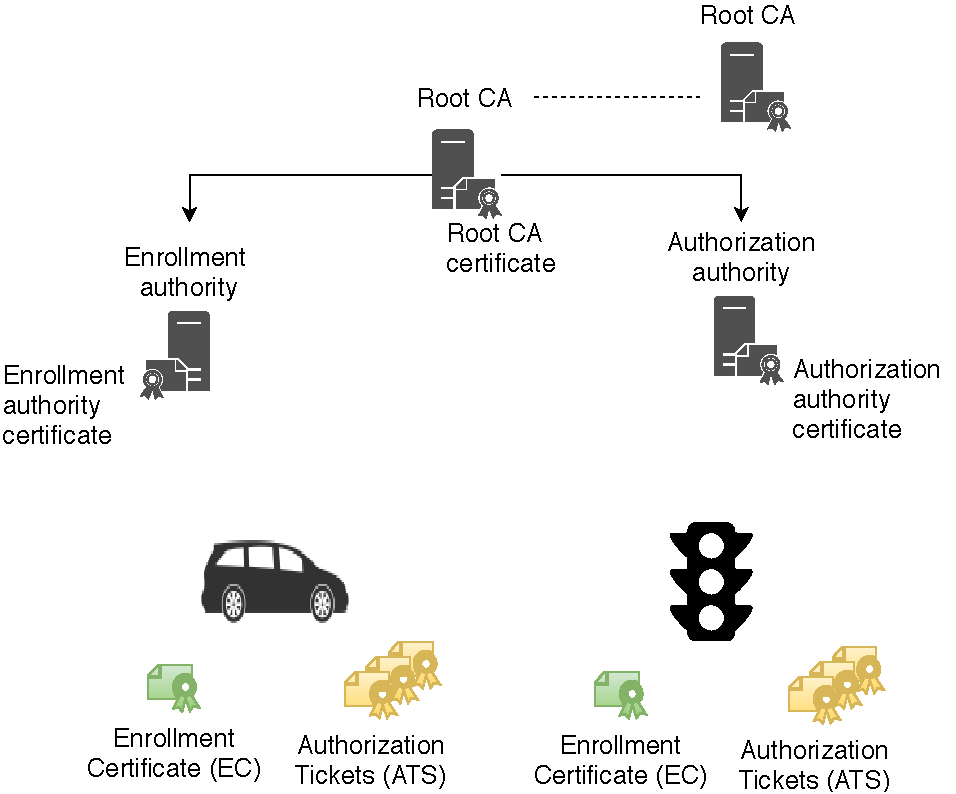
\includegraphics[width=0.8\textwidth]{Figures/ETSI_PKI.pdf}
	\caption{\label{fig:ETSI_PKI}European vehicular PKI architecture.}
\end{figure}

%%%%%%%%%%%%%%%%%%%%%%%%%%%%%%%%%%%%%%%%%%%%%%%%%%%%%%%%%%%%%%%%%%%%%%%%
\subsection{ITS-S Security Life Cycle}
\label{section:life-cycle}

The ITS-S security life cycle is relevant for our solution because through its analysis we are able to understand which stages every vehicle undergoes during its lifetime. Each stage involves a change in the vehicle's state against the PKI. The analysis of such stages allows us to understand when and what information needs to be initialized in the vehicles and transferred between vehicles and the PKI. Specifically, which variables need to be initialized in the vehicles’ OBU at bootstrap, what needs to be done regarding the vehicle enrollment and authorization, and how can we update PKI management information throughout the life cycle of the vehicles.
ETSI TS 102 941 \cite{etsi_privacy} standards specify the ITS-S' security life cycle comprising four stages: the manufacture, enrollment, authorization and maintenance. The first stage of an ITS-S' life cycle is the manufacture, it is at this stage that all the information needed for the enrollment is initialized within the station itself (OBU) and within the EA. The next stage is the enrollment where the ITS-S requests its enrollment certificate from the EA. Having received the enrollment certificate, the ITS-S can now request authorization tickets from the AA. The request for authorization tickets represents the authorization stage. 

When a vehicle is manufactured the OBU and EA need to be initialized. Within the vehicle's OBU, it is necessary to provide information regarding the vehicle's identity and information to allow the vehicle to interact with the PKI. Regarding the identifying information, a unique identifier and a public\slash private key pair to be used for cryptography are created. Optionally, a canonical certificate can be installed which associates the canonical identifier with the public key of the vehicle. In this case, the certificate chain back the root authority needs also to be installed. To allow a vehicle to connect to the PKI, it is necessary to install the network address and public key certificate of the EA and AA that will issue certificates for that vehicle. In addition, the set of known and trusted EA certificates is installed to allow the vehicle to initiate the enrollment process. To grant that such vehicle is able to verify the authenticity of incoming V2X messages, the set of known and trusted AA certificates must also be provided. In order to support vehicle enrollment, within the EA it is necessary to provide information that identifies the manufactured vehicle: a unique vehicle identifier, the location profile information for the vehicle, and the public key that belongs to the vehicle's key pair. In the next sections we study how the European Vehicular PKI operates regarding the provisioning of certificates, their revocation, and how the messages are signed and verified by the user vehicles. Our vehicular PKI must support such operational aspects.

\subsection{Enrollment Process}

Before an ITS-S is able to participate in the V2X communication it must be registered within the PKI. The enrollment request message should be sent from the ITS-S to the Enrollment Authority, to protect the users' privacy the request must be encrypted. According to ETSI TS 102 941 \cite{etsi_privacy} this message should contain the following fields:
\begin{itemize}
	\item{ Message signer information, i.e. the canonical certificate or the public key provided to the ITS-S at bootstrap to globally identify it.}
	\item{ certificate request, i.e. the information to be presented in the enrollment certificate. For example, the ITS-S' public key, start time, end time and other certificate specific data.}
	\item{ The digital signature of the message sender (requesting ITS-S) calculated over all message fields.}
\end{itemize}
After the ITS-S enrollment request the target EA must reply with a successful or failed response message, to protect user privacy the response should also be encrypted. The successful ITS-S enrollment response should contain the enrollment certificate and the chain of certificates back to the originating enrollment CA. In the failed ITS-S enrollment, the response contains the error code i.e. the reason for the unsuccessful enrollment response. 


\subsection{Authorization Ticket Provisioning}
\label{section:at_usage}

Pseudonym certificates are short-lived certificates which express the permissions that a specific enrolled vehicle has on the road while hiding its identity. Consequently, they are refereed as \textit{Authorization Tickets} (ATs) by ETSI. To avoid long-term tracking, a vehicle rotates authentication tickets from its local pool to authenticate V2X messages. However, it needs to request new ATs from the authorization authority once there are few valid ATs stored locally. The update can be done over-the-air or at an authorized dealership (during vehicle maintenance), i.e. roadside-units and workshops can act as a proxy for certificate requests. Because our solution will also use ATs, important decisions must be done regarding the frequency that ATs are provisioned to the enrolled vehicles and how such vehicles rotate certificates from their pool. There is the need to adopt a model that specifies the authorization ticket provisioning. The model used in Europe is defined in CAR 2 CAR Communication Consortium (C2C-CC) \cite{generic_eu}. In this model the required frequency of updates, the delivered level of privacy and security can be expressed by three determining parameters:

\begin{itemize}
	\item{ \textbf{Certificates valid simultaneously:} It can be defined that the requester can use several ATs with the same start and expiry date.} 
	\item{ \textbf{Authorization ticket validity time period:} Is defined by the time between start and expiry timestamps of the ATs.}
	\item{ \textbf{Overall covered time-span:} The time that is covered by the batch of authorization tickets.}
\end{itemize}

A vehicle receives a ``super-batch'' that contains a set of ATs, the duration of the ``super-batch'' is the \textit{overall covered time-span} and is in the order of years. The ``super-batch'' is composed of ``sub-batches'' which contain a sub-set of certificates (e.g., 20) valid for the same time period (e.g., a week). During that week the vehicle uses and reuses the 20 valid certificates. The certificate usage pattern can vary from device to device, e.g. a device could use a certificate for 5 minutes after start-up, then switch to another certificate, and use that either for 5 minutes, or until the end of the journey. Figure \ref{fig:AT_P} illustrates this method. 

\begin{figure}
	\centering
	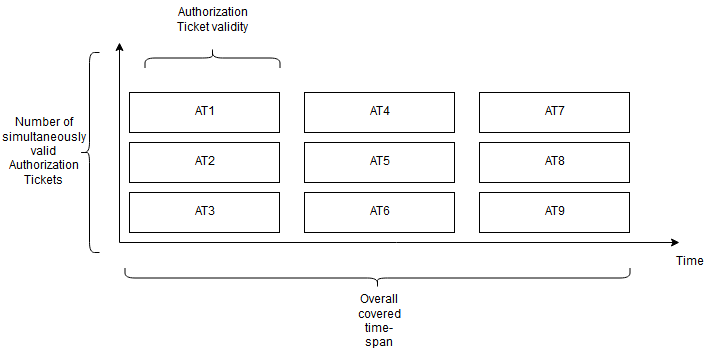
\includegraphics[width=0.8\textwidth]{Figures/AT_P.png}
	\caption{\label{fig:AT_P}Authorization Ticket provisioning model.}
\end{figure}

\subsection{Authorization Ticket Request Process} \label{auth_process}
In this section we study the sequence of messages used by vehicles to request valid ATs in Europe. The solution that we propose will assume such protocol for the simulated vehicles' requests for ATs.
At a high level, a vehicle uses its enrollment certificate to prove its enrollment to the AA, only then the AA can issue the ATs.
The ETSI TS 102 941 \cite{etsi_privacy} standard specifies in detail the message format for the AT request and response. In regards to the process \cite{generic_eu}, the vehicle sends a request to a predefined AA. The request includes the vehicle's enrollment certificate, the certificate of the corresponding Enrollment Authority, and the to be certified public key. To protect user's privacy the enrollment certificate may be encrypted with the public key of the corresponding EA. In this case the AA is not able to create a link between the authorization tickets and the enrollment certificate of a specific vehicle. Consequently, when an AA receives such requests it cannot verify the enrollment of the requesting vehicle. In order to do so, the AA sends a request with the (encrypted) vehicle's enrollment certificate and the calculated AT overall covered time-span (e.g. 1 year) to the correct EA (identified by the EA certificate present in the original request). The EA maintains a database that stores a timestamp marking the deadline which the vehicle will still have valid ATs (calculated using the overall covered time-span of the request). Only if the vehicle's enrollment certificate is valid and no ATs are issued for the time which the vehicle still has valid ATs the AA will get a positive response from the EA validating the enrollment of the vehicle. Upon receiving such response, the AA has the responsibility of issuing the ATs for the vehicle. This procedure prevents a vehicle from requesting ATs for the same time interval from different or the same AAs.


\subsection{Message Signing and Verification}

In this section we analyze how the secured V2X messages are signed and verified by the vehicles. Such information will allow us to correctly test the communications between vehicles in the proposed simulator. In regard to sending messages, the sender of V2X messages signs all outgoing messages with the private key of a valid AT. Afterwards, the message with the appended signature and pseudonym certificate is broadcast. When a station receives a message, the senders authenticity and message integrity is verified by decrypting the signature with the public key from the appended AT. The sender's authenticity is only accepted if verification of the received AT up to a root CA is possible. Vehicles are preloaded with the known and trusted authorization authority certificates at manufacture. However, if the Authorization Authority certificate that corresponds to the received AT is not locally stored, the message receiver cannot validate the sender's authenticity. In this case, the message receiver must create a new message requesting the missing Authorization Authority certificate and send it to the original message sender. Then, the receiver of this request must respond with the Authorization Authority certificate (more details present in Section \ref{standards}).

\subsection{Certificate Revocation}

Sometimes it may be necessary to remove bad actors from the system. This requirement influences the architecture of the PKI, namely there must be an entity responsible for detecting misbehaving actors. Once detected, a bad actor must be removed from the communication. 

In the European solution detecting and preventing misbehavior by means of a misbehavior entity is not yet supported. Revocation is done in respect to the long-term enrollment certificate of ITS-S and CA certificates. ITS stations are eventually removed from the system by rejecting new requests for ATs. In this concept the EA links the revocation information of the vehicle to its long-term enrollment certificate. If the vehicle requests new ATs then the AA forwards the request to the respective EA which checks the revocation information of the requester. In respect to the revocation of any CA certificate a distributed \textit{Certificate Revocation List} (CRL) is used. In this scheme, the CA certificates that are compromised are revoked manually by the PKI administration; the certificate identifier is posted in the CRL and signed by the root CA; finally, the CRL is distributed inside the PKI backbone and connected ITS stations. The CRL for EA and AA certificates is defined in ETSI TS 102 941 \cite{etsi_privacy} standard.

\section{Overview of the American Vehicular PKI Solution} \label{us_pki}
In this section we provide an overview of the Security Credential Management System as a matter of reference. Although this theses follows the European PKI solution, it is relevant to reference the American vehicular PKI in order to understand the main differences and similarities between solutions.
In comparison to the architecture of the European vehicular PKI the American counterpart is noticeably more complex. However, it shares some similarities with the European vehicular PKI. The main differences include an increased focus on privacy against attacks from SCMS insiders, the handling of certificate revocation, and the method for provisioning certificates based on the butterfly key expansion algorithm. 

\subsection{American Vehicular PKI Architecture}
\bigbreak
SCMS considers an hierarchical structure as we can see in Figure \ref{fig:SCMS_PKI}. Comparing with the European vehicular PKI architecture, there are some components with a similar function and others that introduce new functionality. In regard to the similar components, SCMS assumes a \textit{Root CA}, an \textit{Enrollment CA}, and a \textit{Pseudonym CA} (PCA) which corresponds to the authorization authority in the European architecture. As to the remaining components, their functionality is as follows:

\begin{itemize}
	\item \textbf{Device Configuration Manager (DCM):} Provides authenticated information about changes in the configuration of SCMS's components, for example an authority changing its certificate. It is also used to inform an enrollment CA that a device is eligible to receive enrollment certificates.
	\item \textbf{Registration Authority (RA):} Validates, processes, and forwards requests for pseudonym certificates to a pseudonym CA.
	\item \textbf{CRL Store (CRLS):} Stores and distributes CRLs. CRLs are signed by the CRL Generator.
	\item \textbf{CRL Broadcast (CRLB):} Broadcasts the current CRL, may be done through road side units or satellite radio system, etc.
	\item \textbf{Linkage Authority (LA):} The main goal of this component is to improve certificate revocation. LAs generate linkage values, which are used in the certificates and support efficient revocation (more on this later). There are two LAs in the SCMS, referred to as LA1 and LA2. The splitting prevents the operator of an LA from linking certificates belonging to a particular device. 
	\item \textbf{Location Obscurer Proxy (LOP):} The main goal of this component is to improve the security against SCMS insiders. The LOP hides the location of the requesting device by changing source addresses. Additionally, when forwarding information to the Misbehavior Authority (MA), the LOP shuffles the reports to prevent the MA from determining the reporters’ routes.
	\item \textbf{Misbehavior Authority (MA):} Processes misbehavior reports to identify potential misbehavior by devices, and if necessary revokes and adds devices to the CRL. It also initiates the process of linking a pseudonym certificate to the corresponding enrollment certificates, and adding the enrollment certificate to an internal blacklist.
	\item \textbf{Request Coordination (RC):} Ensures that a device does not request more than one set of pseudonyms for a given time period. It coordinates activities between different RAs.
\end{itemize}

An early version of SCMS has already been implemented, operated and tested in the safety pilot project \cite{safty_pilot}. Safety pilot is a scaled-down evaluation of V2X that uses real vehicles and roadside infrastructure in order to understand the safety benefits of connecting vehicles. SCMS documentation can be found in \cite{scms_doc}

\begin{figure}
	\centering
	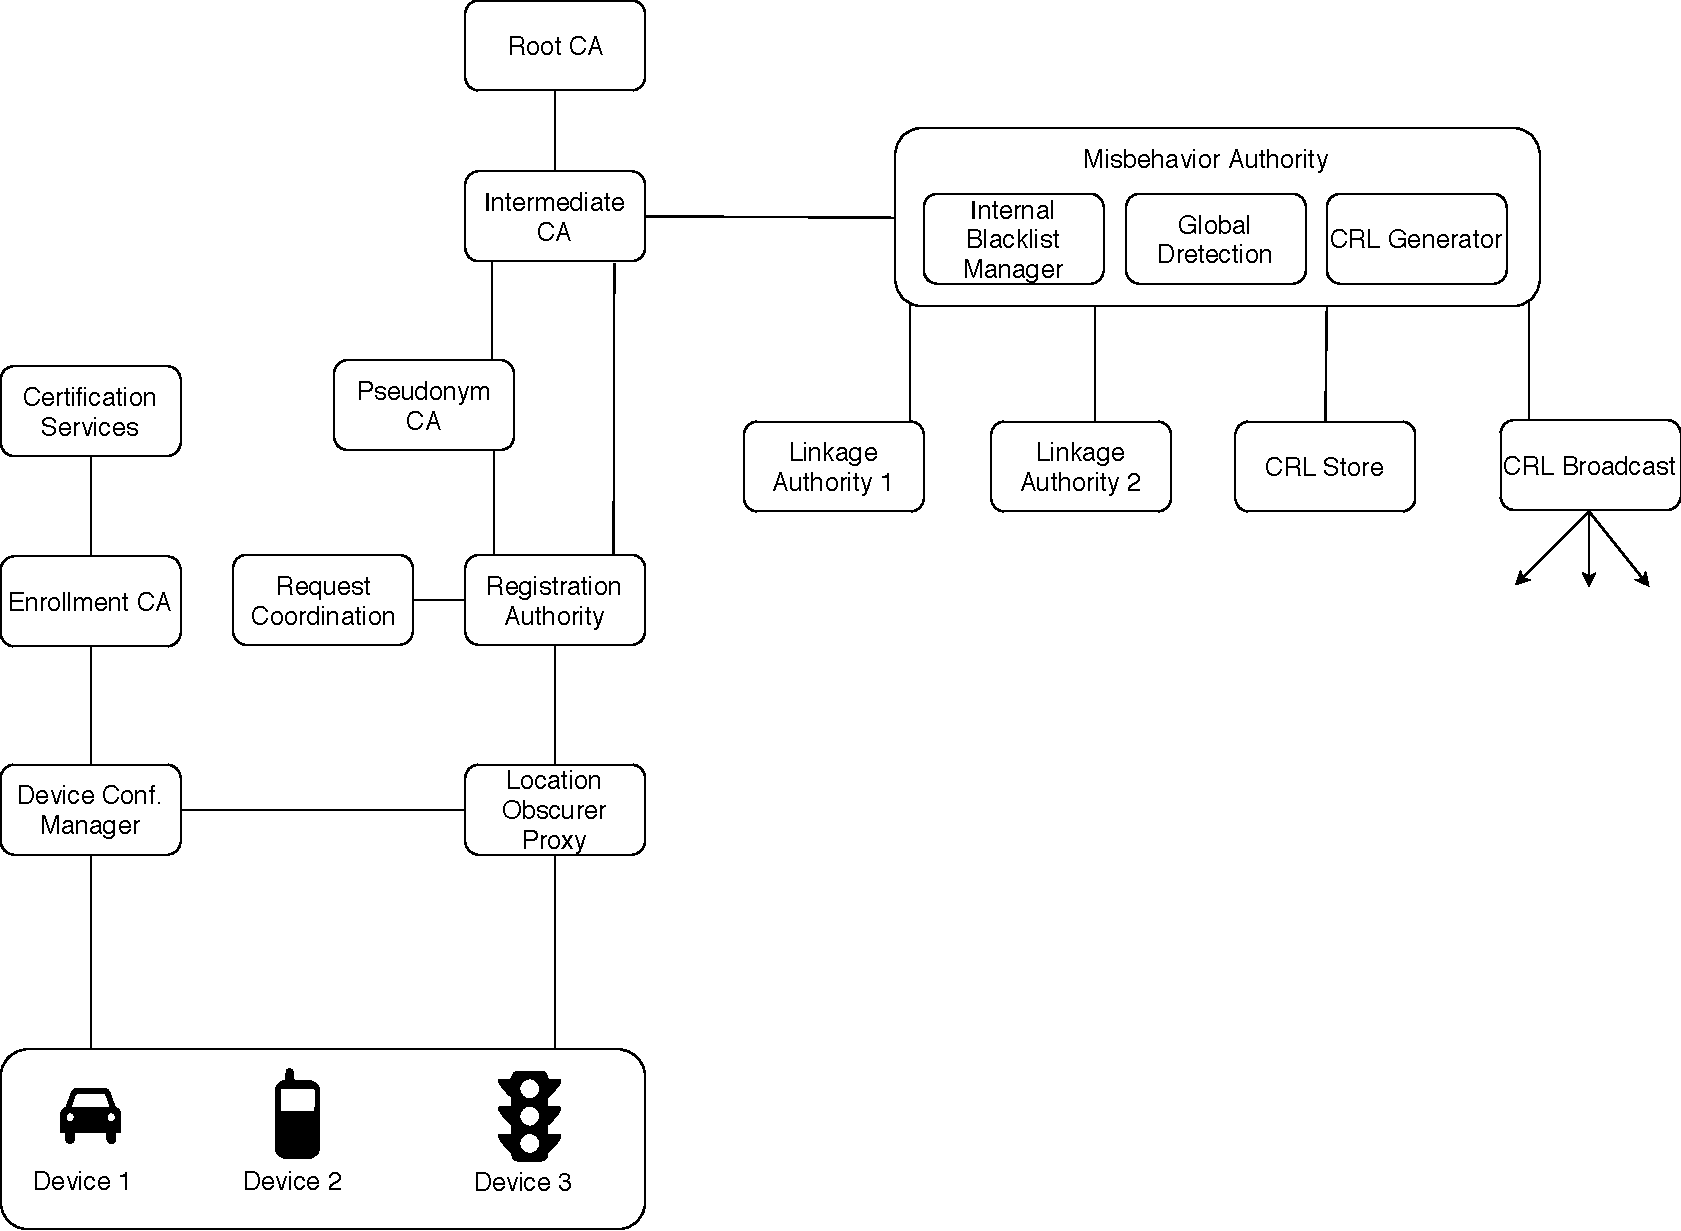
\includegraphics[width=0.8\textwidth]{Figures/SCMS_PKI.pdf}
	\caption{\label{fig:SCMS_PKI}SCMS overall system architecture.}
\end{figure}

\subsection{Pseudonym Certificate Provisioning Model}
\bigbreak
Regarding the model used for provisioning pseudonym certificates, the SCMS assumes the same model as in CAR 2 CAR Communication
Consortium \cite{generic_eu} (European solution) illustrated in Figure \ref{fig:AT_P}. The proposed parameters for this model are:
\begin{itemize}
	\item \textbf{Certificate validity time period:} 1 week.
	\item \textbf{Certificates valid simultaneously (batch size)}: 20 to 40 certificates.
	\item \textbf{Overall covered time-span (super-batch size):} 1 to 3 years.
\end{itemize}

\subsection{Pseudonym Certificate Request Process}

The request for pseudonym certificates in itself is different from the European solution. For this the
butterfly key expansion algorithm \cite{scms} is used. Butterfly keys allow a device to request an arbitrary number of certificates, each encrypted with a different encryption key and each containing a different signing key. The request contains only one seed for the verification public key, one seed for the encryption public key, and two expansion functions. Without butterfly keys, vehicles would have to send a signing key and a unique encryption key for each requested certificate. Butterfly keys reduce upload size, allowing requests to be made even in suboptimal connectivity conditions, and also reduce the computation to be done by the vehicle to calculate the keys. More information about the request process can be found in \cite{scms}.


\subsection{Misbehavior Reporting}

In contrast to the European PKI, the American PKI supports misbehavior reporting by user vehicles. This feature aims to improve the security against SCMS outsiders by reporting their malicious messages. 
Devices will send misbehavior reports to the MA via the LOP which will obscure the source and shuffle the reports from multiple reporters, this is done to prevent the MA from reconstructing the reporter’s path based on the reports. The format of a misbehavior report is not fully defined yet, but a report will potentially include reported messages in addiction to the reporter’s signature and certificate, and will be encrypted by the reporter for the MA.

\subsection{Global Misbehavior Detecting and Revocation}

The algorithms necessary for global misbehavior detection have not been developed at the time of this writing. However, the interface which allows SCMS components to retrieve linkage information is already specified.
Revocation is tightly bound to the linkage information which basically allows the MA to find whether multiple reported messages point to the same device.
The revocation process is described step-by-step in \cite{scms}. In this section we learned about the European and American vehicular PKIs and about their most relevant operational aspects. In the next section we present the standards which shape the formats of the certificates and messages used in the European vehicular PKI.

\section{Secured Message and Certificate Formats Standard}\label{standards}
One of the main concerns of V2X communication is the ITS interoperability. Standardization of the communication protocol becomes fundamental with so many vehicles from different manufacturers using the road and sharing information. To achieve this goal there are dedicated work groups within standardization organizations that address security and privacy concerns. While ETSI Automotive Intelligent Transport Systems represents the main standardization stakeholders in Europe \cite{etsi_workgroup}, IEEE 1609.2 represents the main standardization stakeholders in the U.S \cite{iee_formats}. Such standardization efforts are the basis of the security and privacy of the European and American vehicular PKI solutions respectively. A survey about recent standardization activities in Europe (ETSI) has been done by IEEE in \cite{wow}.

Regarding the secured message and certificates formats. IEEE 1609.2 \cite{iee_formats} standard defines the formats for secured V2X messages and public key certificates to be used in SCMS. In this standard the V2X message authenticity and integrity are based on the \textit{Elliptic Curve Digital Signature Algorithm} (ECDSA). The message confidentiality protection is based on AES symmetric encryption (AES-CCM mode). For the transport of symmetric keys the \textit{Elliptic Curve Integrated Encryption Scheme} (ECIES) is used. ETSI TS 103 097 standard \cite{etsi_formats} assumes the same cryptosystem as IEEE 1609.2 and presents security profiles for the messages and certificates also based on the IEEE 1609.2 standard. This means that ETSI's profiles are specific types of messages and certificates which are based on particular options available on the definitions of the base standard. For example, ETSI TS 103 097 uses the definition of possible fields that a certificate may contain (the format) present in IEEE and, based on these options, builds the specific profiles (the necessary fields) for the root CA certificates, authorization tickets, enrollment certificates, and other certificates to be used in the European solution. The same process applies with the profiles for the secured V2X messages. 

The V2X ecosystem that we propose will be primarily based on the European PKI. Consequently, it is relevant that we understand the contents of the secured V2X messages and the certificates used by it. In order to do so, we provide an overview of the ETSI TS 103 097 standard. 

\begin{figure}
	\centering
	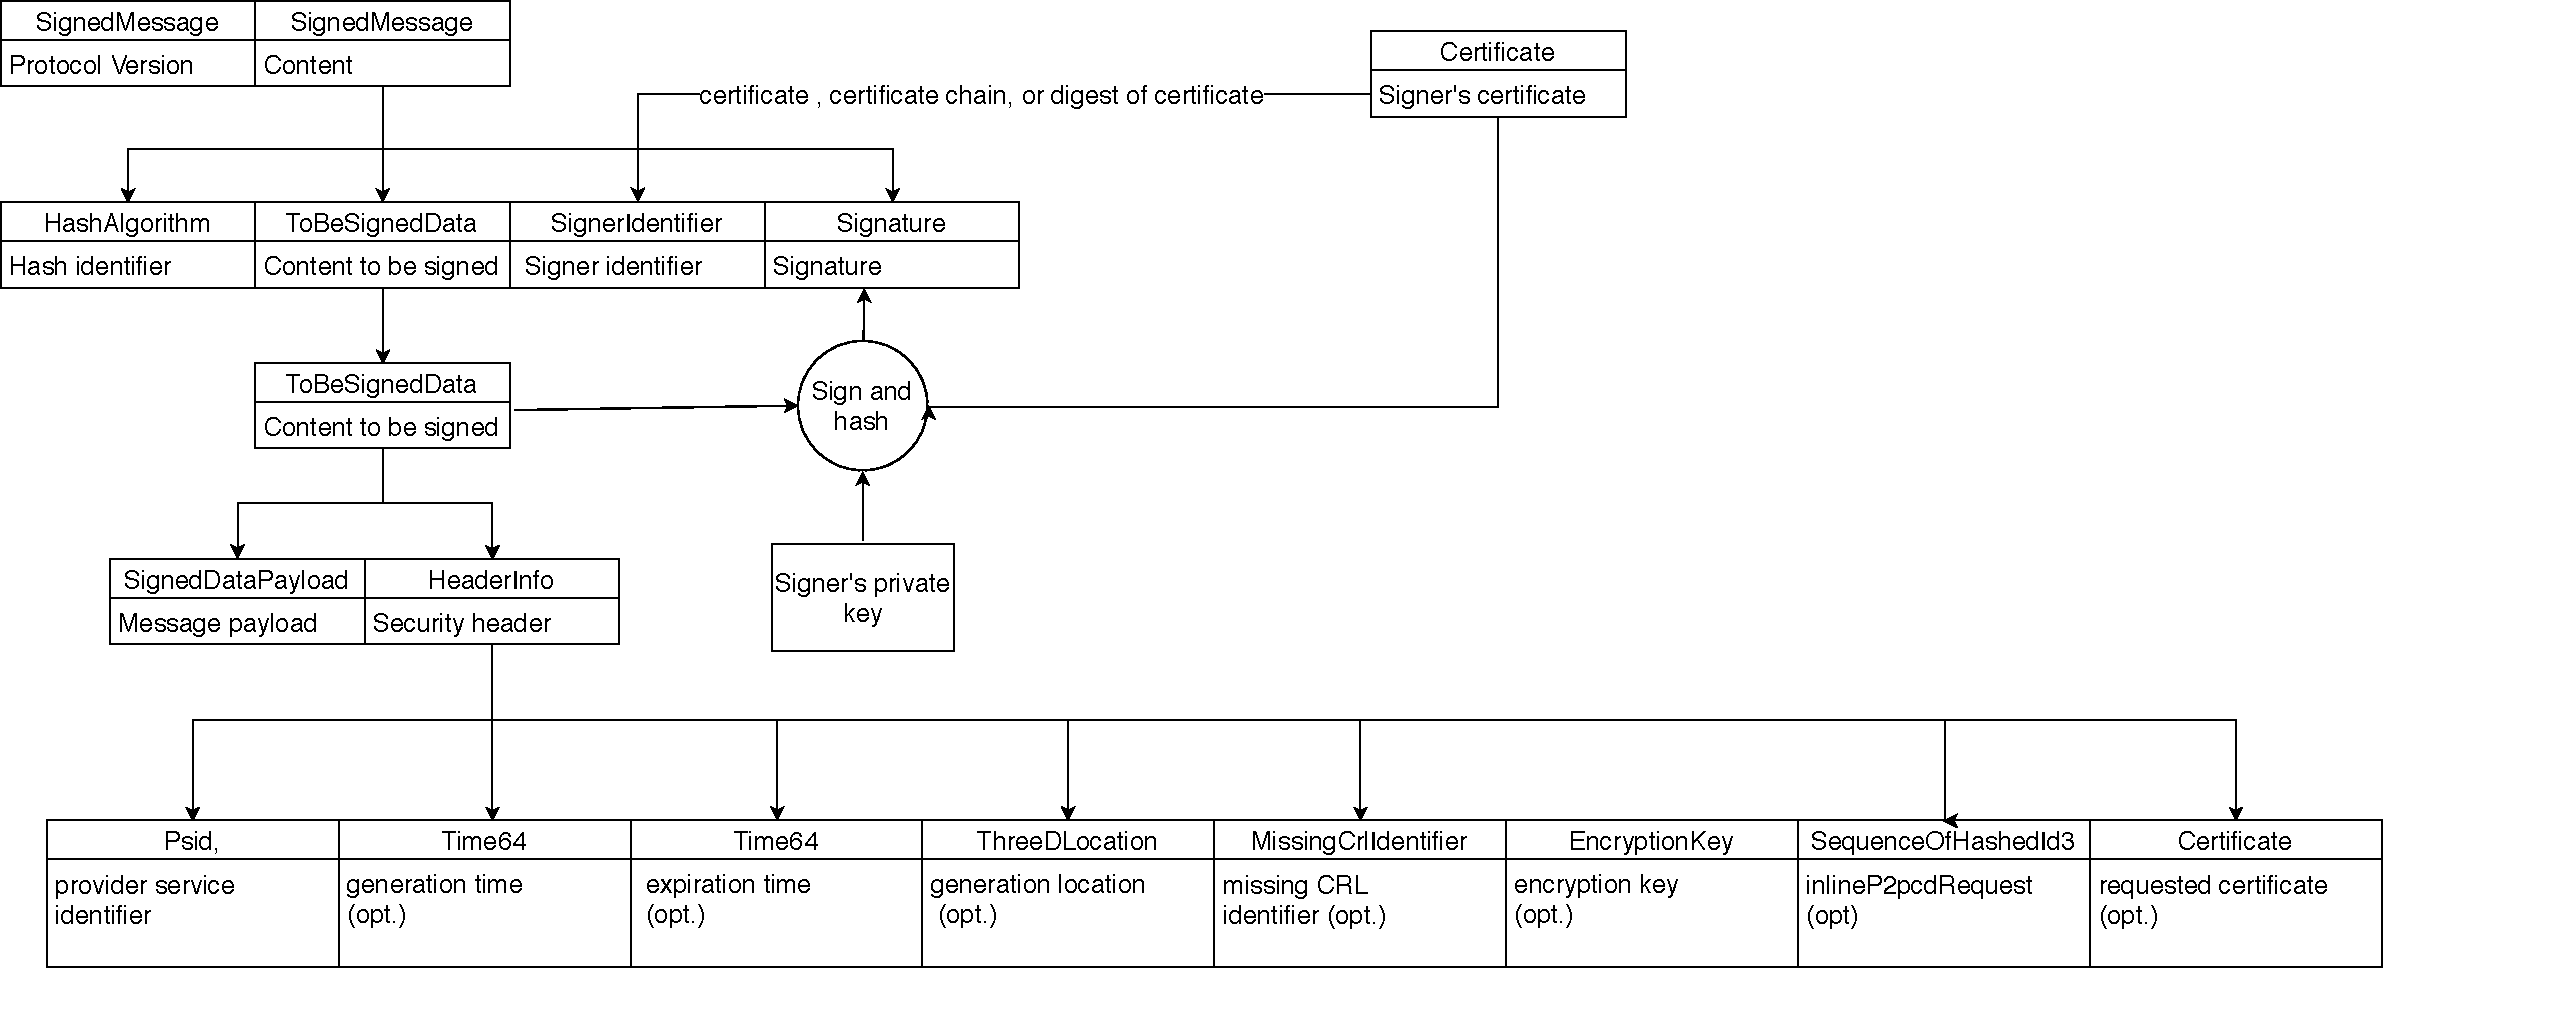
\includegraphics[width=1.1\textwidth]{Figures/message_format.pdf}
	\caption{\label{fig:signed_message}IEEE 1609.2 signed message format used by ETSI TS 103 097.}
\end{figure}

\subsection{Secured Messages Formats}
Figure \ref{fig:signed_message} depicts the format of a secured message. Generally a message can be transmitted as unsecured data, signed, encrypted, or signed and encrypted data. In the case of road security messages, the message should be signed and thereby include the hash algorithm, the content to be signed, the signer identifier, and the signature itself. Such security messages need to carry the signing certificate (authorization ticket) to reduce the processing delay at the receiver side. However, in order to reduce the network bandwidth consumption it is possible to include in the message a reference to the signing authorization ticket. For this purpose, the message signer identifier contains the certificate identifier as the 8 bytes certificate digest instead of the full certificate. 

The content to be signed includes all the message components that will be protected by the signature. Such components are the security header and the message payload. The security header includes components that are relevant for the security layer, such as the provider service identifier and some optional message validation data (generation time, expiration time, generation location, missing CRL identifier, encryption key, \textit{inlineP2pcdRequest,} and requested certificate).



A message is signed by an authorization ticket, which is turn is signed by an authorization authority certificate. Consecutively the authorization authority certificate is signed by a higher authorization authority certificate. The chain ends at a root CA certificate which issued itself. At a high level, at least one certificate in this chain must be known and trusted by the receiving station in order for it to be able to trust an incoming message.

The message receiver needs to be able to construct a chain from the message signing certificate to a known root. However, vehicles are constantly rotating authorization tickets to sign safety messages, normally exchanging only a reference to that certificate (authorization ticket hash). In addition, in many cases vehicles share the road with previously unknown vehicles for the first time. There needs a peer-to-peer (p2p) mechanism to distribute certificates on the road. This mechanism in embedded into the secured messages, specifically the receiver can use the \textit{inlineP2pcdRequest} component of a message to request unknown certificates from other senders. This functionality allows us test the correctness, performance and overhead of the distribution of unknown authorization tickets on the road.

\subsection{Secure Messages Profiles}
In the previous section we learned about the possible message components and their meaning. Here, we analyze the already standardized safety message profiles for the \textit{cooperative awareness messages} and \textit{decentralized environmental notification messages}. For each type of message, we analyze their goal, how they are sent, and how they are received by the vehicles. The proposed simulator will implement the V2X communications between simulated vehicles. As such, it assumes these two specific types of messages secured by the ATs provided by the proposed vehicular PKI.

\subsubsection{Security Profile for Cooperative Awareness Messages}
\textit{Cooperative Awareness Messages} (CAM) are messages that are exchanged between ITS-S. As the name implies, these messages are used to achieve cooperative awareness on the road. This means that road users such as vehicles (cars, trucks, trains, etc.), road-side units (traffic lights, gates, barriers, etc.) and people are aware of each other's positions, speed and other dynamic variables. To achieve this goal, it is essential that this type of messages is periodically broadcast by each road user to all its neighbors. CAMs are used to support traffic management and safety services. In the normal cases CAMs are sent multiple times per second with the component signer identifier containing the reference of the signing authorization ticket (8 byte certificate digest). However, in order to distribute the currently used AT, every second a CAM is sent with the signer identifier containing the full certificate. If a vehicle receives a CAM signed by a previously unknown AT, it should include the currently used AT immediately in its next CAM, instead of including just the digest. In this case, the timer for the next inclusion of the full certificate should be restarted to one second. 

Besides distributing the currently used AT a vehicle also needs to request the unknown certificate present on the revived CAM for message verification purposes. Specifically, if a vehicle receives a CAM with the signer identifier containing an unknown certificate digest, then it will include that digest in the component \textit{inlineP2pcdRequest} of its next CAM to broadcast the request for the full certificate. 
It is also possible for a vehicle to receive a CAM containing the full signing authorization ticket but this certificate is signed by an unknown authorization authority certificate. In this case the vehicle should include in the \textit{inlineP2pcdRequest} of its next CAM the digest of the unknown authorization authority certificate which is present on the AT itself (see more in Section Certificate formats).

If a vehicle receives a CAM containing a request for an unknown certificate i.e. with the component \textit{inlineP2pcdRequest} on the security header, then the vehicle searches the list of certificate digests existing in that component. If the digest of the currently used authorization ticket is found in that list, then it includes the full certificate in the component signer identifier of its next CAM instead of the digest. In the case that a vehicle finds a digest referencing a valid authorization authority certificate in that list, it should include such certificate in the component requested certificate of its next CAM to broadcast the response. It is possible that multiple neighbor vehicles have stored the requested AA certificate, in order to prevent unnecessary broadcast responses, a vehicle only includes the AA certificate in its next CAM if before the generation of this message no other CAM was revived containing the AA certificate in the component requested certificate.


\subsubsection{Security Profile for Decentralized Environmental Notification Messages} 
\textit{Decentralized Environmental Notification Messages} (DENM) are messages designed to provide asynchronous warning notifications to vehicles. DENMs are event triggered and are broadcast to notify the users of a hazardous event. For example, an emergency vehicle approaching or an accident on the road. These messages have to be broadcast to all users affected by the event, sometimes multiple hops are needed to achieve this.

In order to reduce the verification delay at the receiver side CAMs are always sent with the full signing authorization ticket in the signer identifier. Because it is important for vehicles to know were the event occurred, these messages will always include in the header the generation location.

\subsection{Certificate Formats}\label{cert_formats}
In the previous sections we have seen the secured message formats and profiles, which are relevant for V2X communications. In this section we introduce the existing certificate formats, which are relevant to secure such messages. Our goal is to encode such formats in a Java package and then integrate it into mPKI.


The certificate formats include profiles for the root CA, enrollment authority, authorization authority and end-entities certificates (authorization tickets and enrollment certificates).
Generally a certificate is composed of the issuer identifier, certificate identifier, application permissions, permitted geographic location, start of the validity time, expiration time, public key and the signature. In order to construct the certification chain, each non-root certificate carries the issuer identifier which is a reference (8 byte digest) that points to the certificate that belongs to the issuer CA. For example, authorization tickets carry the digest of their corresponding authorization authority certificate. The certificate identifier is a unique name that identifies the certificate's host (i.e. name of a certification authority in the case of CA certificates). The application permissions contain one or more pairs of \textit{Provider Service Identifier} (PSID) and \textit{Service Specific Permissions } (SSP). While PSID indicates a specific service, message or application the SSP indicates the permissions within that service. For example, there may be an SSP value associated with PSID of a CAM that indicates that the vehicle is privileged to send such message for a specific vehicle role (e.g emergency vehicle) or for a specific roadside unit (e.g traffic lights).

\subsection{Signed Message Validity Checks}

Before a vehicle is able to trust an incoming message it must check the message's validity. This is done by verifying that no certificate in the certification chain is revoked and the signing certificate chains to an already trusted CA certificate.
Also, the signature present in the message can be verified using the public key expressed in the certificate. The message payload must be consistent with the permissions expressed in the certificate (by the PSID/SSP pairs). Finally, the message must not be expired, i.e. the message validity is within the certificate's validity period and the message was generated within the permitted geographic location of the signing certificate. Figure \ref{fig:relation} depicts the consistency between a signed message and the signing authorization ticket.

\begin{figure}
	\centering
	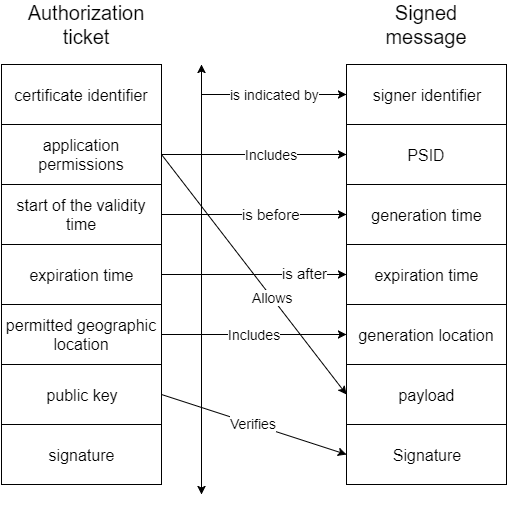
\includegraphics[width=0.5\textwidth]{Figures/relation.png}
	\caption{\label{fig:relation}Relation between a signed message and the signing certificate.}
\end{figure}


\section{Overview of the ITS Simulators}\label{simulators}
Implementing V2X communication is expensive and may prove to be dangerous to test using real vehicles. Furthermore, to properly measure the benefits of V2X communication we need to evaluate it at a large scale, for example hundreds of ITS-S. Before we can conduct a field test, a simulation framework which is able to test the communications between vehicles and infrastructure of whole cities is needed. This implies simulation at three different domains: traffic simulation to generate the road networks and traffic demand; network simulation to allow vehicle connectivity by wireless technology (e.g. IEEE 802.11p
DSRC, and IEEE 1609.4 WAVE) \cite{network_vehicle} \cite{network_vehicle2}; and ITS application simulation to trigger the communication. 
In this section we list some of the most known ITS simulators. A survey on the most known simulation tools and techniques for vehicular communications and applications can be found in \cite{sims}.

\subsection{Vehicle Mobility and Networking Simulators} 
Vehicle mobility simulators are specialized in generating the road networks and traffic demand. At this level of simulation it is important to support: a realistic representation of traffic flow that may range from a single road junction to a whole city; the support for adding new functionality and integration with other simulation tools (e.g. an interface that allows retrieving traffic simulation data and control the simulation using external functions). In this category of simulators there are two promising candidates: SUMO \cite{SUMO} and VISSIM \cite{vissim}. Network simulators have the responsibility of representing the network protocols that transmit ITS information through the VANET, to a back-end or Internet service. In this category of simulators there are three promising candidates: ns-3 \cite{ns3}, OMNeT++ \cite{omnet} and JiST\slash SWANS \cite{jist}.


\subsection{Integrated ITS Simulators}
Integrated ITS Simulators are frameworks that couple different domain simulators in order to create a functional V2X environment. At this level of simulators it is important to support a bidirectionally-coupled simulation \cite{bidirectional} of road traffic and network traffic (the mobility of vehicles affects communication and vice-versa). In this category of simulators there are three promising candidates: Veins \cite{bidirectional}, iTETRIS \cite{iTetris}, and VSimRTI \cite{vsimrti}.


\section{Discussion}
In this section we provide a brief overview of the vehicular PKI solutions presented and analyze their advantages and disadvantages.
We have seen that in Europe exists \textit{A Generic Public Key Infrastructure for Securing Car-to-X Communication} \cite{generic_eu} and in America exists the \textit{Security Credential Management System} \cite{scms}. In regard to the European PKI, the first disadvantage comes in the vehicle's request for authorization tickets. This solution assumes that every vehicle has to calculate a list of keypairs containing one signing and verification key for each of the requested authorization tickets. Since vehicles typically request a bundle of certificates to be used in a timespan of years, the generation of keys results in an increased computing overhead within the OBU whenever a vehicle needs to request new Authorization tickets. In addition, this process also increases the size of the request, which has to contain all the verification keys. The second disadvantage comes in the revocation of certificates. The European PKI does not consider distribution of CRLs containing authorization tickets within the vehicular network. As a result, this solution allows a window of vulnerability where malicious vehicles have their enrollment certificate revoked but still have a pool of valid authorization tickets, which allows them to send authenticated message for the duration of that pool. Although this system has these disadvantages it provides a simple architecture that is compatible with mPKI and is based on the most accessible standards. These advantages provide us with a good starting point for the implementation of the proposed solution. Regarding the American solution, the main disadvantages are that the underlying standard is paid to obtain and most importantly, the complexity of its architecture and protocol makes it much less compatible with mPKI. 

Having in mind the advantages and disadvantages of the existing vehicular PKI solutions, we decided to base our PKI solution on the European vehicular PKI. However, as we have discussed before, the European vehicular PKI is a generic concept. For this reason it cannot be immediately implemented in mPKI. For example, one of the main aspects that is not specified in this solution is the interface between vehicles and CAs. Next, we present the changes to the European vehicular PKI that we assumed in order to define our V2X environment.

\section{Summary}
In this chapter we have studied the state-of-the-art PKIs used in the identity management of vehicles during V2X communications in Europe and America. We started by overviewing the architecture of such solutions, then approached some operational aspects needed to support a V2X environment. We Finalize this chapter by providing detailed overview of the standards behind the European PKI, and the existing ITS simulators. In the next chapter, we present our V2X environment which is based on the European PKI and standards. We start by overviewing its architecture, then we detail its implementation. % file "Thesis_Background.tex"
\cleardoublepage

%%%%%%%%%%%%%%%%%%%%%%%%%%%%%%%%%%%%%%%%%%%%%%%%%%%%%%%%%%%%%%%%%%%%%%%%
%                                                                      %
%     File: Thesis_Implementation.tex                                  %
%     Tex Master: Thesis.tex                                           %
%                                                                      %
%     Author: Andre C. Marta                                           %
%     Last modified :  2 Jul 2015                                      %
%                                                                      %
%%%%%%%%%%%%%%%%%%%%%%%%%%%%%%%%%%%%%%%%%%%%%%%%%%%%%%%%%%%%%%%%%%%%%%%%
\chapter{Proposed Solution}
\label{chapter:implementation}
In this chapter we start by providing an overview of the system's architecture. For each of the components, we analyse their basic functions and how they connect with each other. In the final part of this chapter we discuss the implementation of such components by describing the most important implementation decisions and the technologies adopted.


%%%%%%%%%%%%%%%%%%%%%%%%%%%%%%%%%%%%%%%%%%%%%%%%%%%%%%%%%%%%%%%%%%%%%%%%

\section{Overview of the System Architecture}\label{section:architecture}
Our solution is primary based on the European vehicular PKI and ETSI's standards. As such, the architecture of our PKI is similar to that of A Generic Public Key Infrastructure for Securing Car to-X Communication \cite{generic_eu} that uses the certificates and message formats standardized by ETSI \cite{etsi_formats} to secure V2X communications, as specified in Section \ref{section:european_pki}. In regards to the software needed to support such PKI, Figure \ref{fig:system_arch} provides an overview of its main components.

\begin{figure}[h]
	\centering
	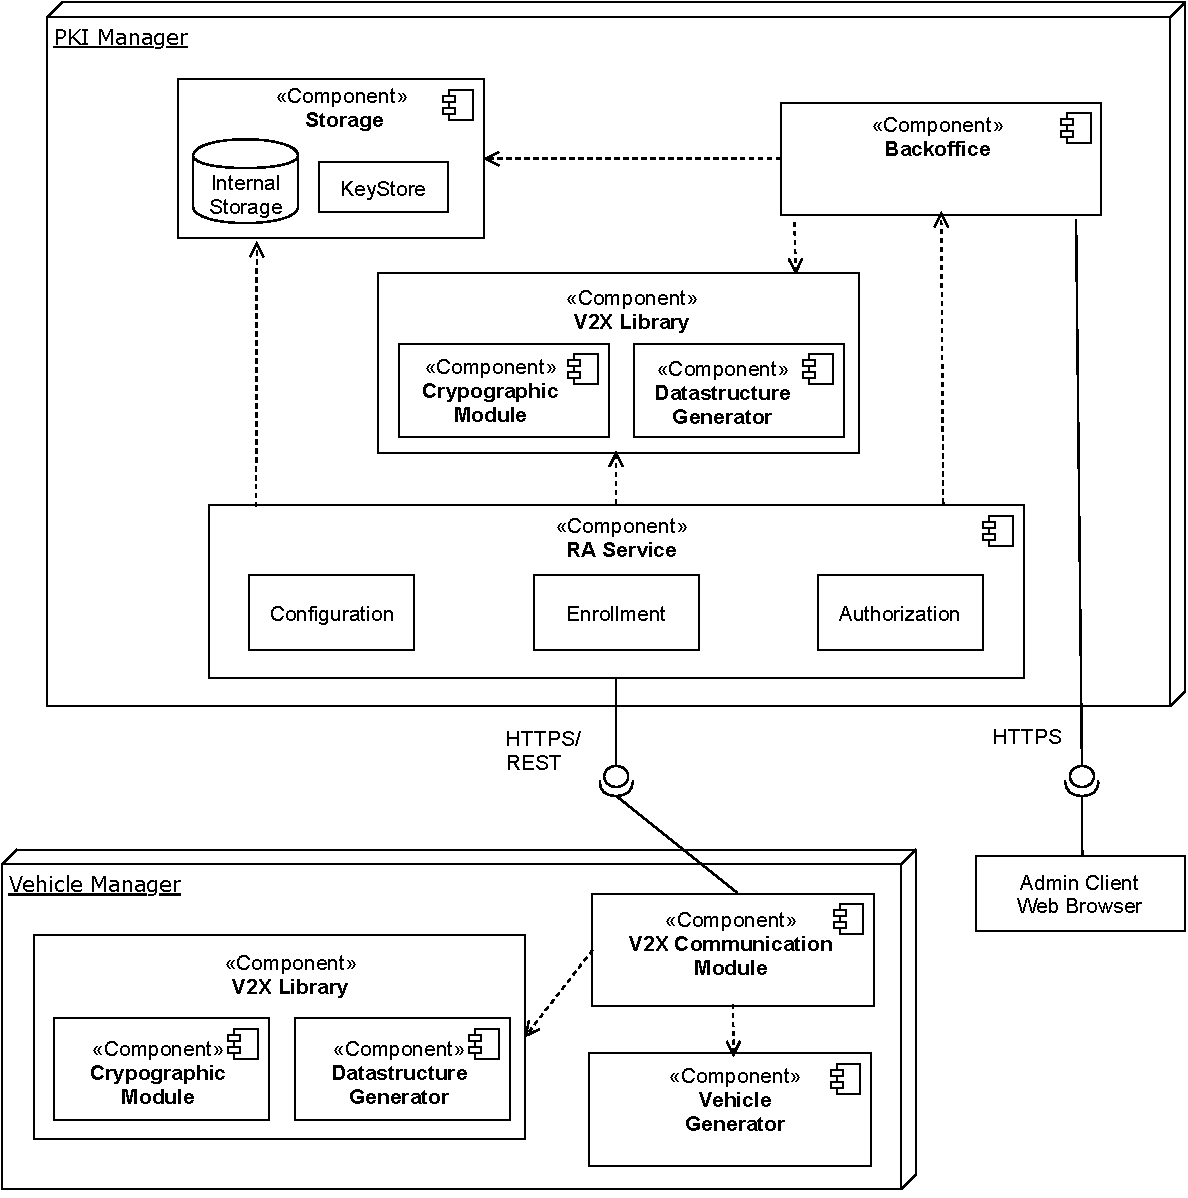
\includegraphics[width=0.8\textwidth]{Figures/arquitetura}
	\caption{\label{fig:system_arch}Overall system architecture.}
\end{figure}

\subsection{System Components}

\paragraph{V2X Library}
\label{section:model}

The V2X Library is designed as a software library package. Its main goal is to create all the data structures specified in the latest version of the ETSI TS 103 097 standard. Such structures combine to form the certificates and messages that are used by the vehicles and PKI. In addition to this, the library also allows is users (PKI Manager and Vehicle Manager) to perform cryptographic operations related with the generation of certificates, signature of messages as well as their verification. The usage of this library allows the PKI Manager and Vehicle Manager to perform such operations in conformance with the approved standards and algorithms.

\paragraph{PKI Manager}
\label{section:model}

The PKI Manager is a web application that functions as a backoffice to the PKI. Such application aims to provide administrative services related to the creation and storage of the vehicular PKI. For example, it enables an admin user to log in and create new CAs, their cryptographic keys and certificates. The PKI Manager allows the creation and configuration of a new PKI or even change the structure of an already existent PKI. This application is connected to a database and KeyStore to provide persistence regarding the PKI information.


\paragraph{RA Service}
\label{section:model}

The RA Service is designed as an API (Application Programming Interface) of the PKI Manager, its main goal is to act as proxy between the vehicles of the Vehicle Manager and the CAs existing on the PKI Manager. The RA has two responsibilities: verifying the vehicle's identity and supporting their requests for enrollment certificates and authorization tickets. The former task requires the RA to perform an initial vehicle configuration, much like authentication, the goal is to “remember” and securely identify each connection to an already configured vehicle. The later task involves sending such requests to the correct CAs for certificate issuing and responding to the vehicles with the requested certificates. The RA Service uses encryption and digital signatures to ensure that the exchange of certificates is secure and the privacy of the end-entities is protected.

\paragraph{Vehicle Manager}
\label{section:model}
As the name suggests, the Vehicle Manager aims to manage the vehicles that will participate in V2X communication. This application runs on its own process and can be configured to create a given number of vehicles each as a client of the RA Service. Once created, the vehicles can contact the RA Service in order to request the end-entity certificates. Only with this initial configuration done, the vehicles are able to start communication with each other in respect to the Vehicle Manager configuration.

\subsection{Communication}
Now that we have seen components of the project and what they do individually, it is time we study how they interact with each other and how is the communication organized. 
As we can see from Figure \ref{fig:system_arch} we assume a client-server architecture, where the server is the PKI Manager and the Vehicle Manager acts as the client. On the server-side, the client requests will enter through the RA Service API, which then communicates with the back end and V2X Library to access the PKI services. As the RA Service is part of the PKI Manager project, the communication with the back end is achieved through simple service calls. Regarding the V2X Library, because this component exists on a different project we used it as a dependency of the server. The V2X Library is a Maven project, so it is possible to include it as one of the server's dependencies, which gives the server access to all the public classes and methods that the V2X Library has to offer. With this information is possible to create an interface on the server-side specifying the methods that will be used by the server as services of the Library. For example, generate a certificate or message, or verify them. Regarding the communication between the server and client, the HTTPS protocol is used to ensure protection of the sensible data that will be exchanged between them. Within the client, the same process is used for the usage of the V2X Library's services.



\subsection{Protocol} \label{protocol}
The interaction between the Vehicle Manager generated vehicles and the PKI is divided into several phases. For the definition of such phases, we assumed the vehicle's life cycle as defined in Section \ref{section:life-cycle}. Essentially, vehicles use the information installed at manufacture time to request the enrollment credential, later using this credential in order to request authorization tickets to start V2X communications. As seen in Figure \ref{fig:system_arch}, the only way that a vehicle can reach the CAs on the PKI Manager is through the RA Service. Specifically through the RA's services of \textbf{configuration}, \textbf{enrollment} or \textbf{authorization}, each of these services represents a phase in the vehicle to PKI interaction. The SSL protocol is used to secure the integrity, privacy and authenticity of the sensitive data that is transmitted during by the Vehicle Manager and RA Service communications.

\begin{figure}[t]
	\centering
	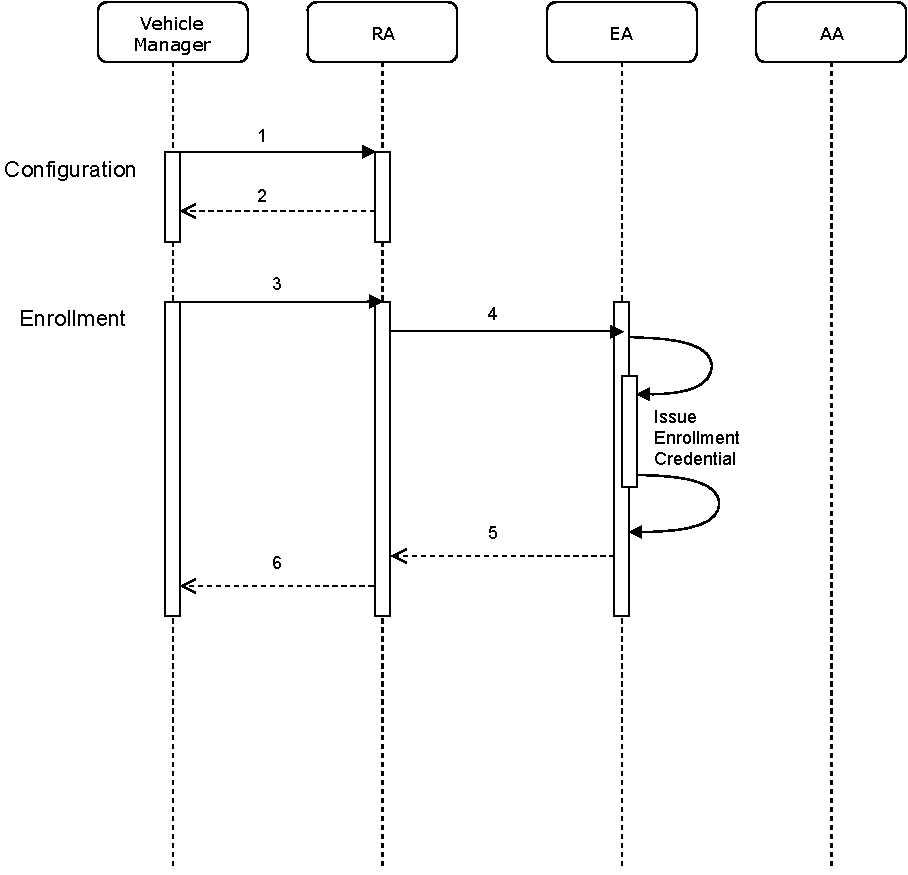
\includegraphics[width=0.8\textwidth]{Figures/protocolo_1}
	\caption{\label{fig:protocol_1}Vehicle configuration and enrollment process flow.}
\end{figure}

\subsubsection{Vehicle Configuration} \label{conf}
The first phase is the configuration. This phase aims to support the vehicle and RA configuration at vehicle manufacture time. Specifically, when the Vehicle Manager is generating new vehicles it uses this service in order to register them and to provide such vehicles with the information regarding the PKI. As we can see from message 1 to 2 represented on Figure \ref{fig:protocol_1}, first the Vehicle Manager starts this phase by sending messag1 containing the canonical public key and ITS identifier of a newly generated vehicle. The RA stores this information in its database and responds with the the PKI information. The secure communication channel between the Vehicle Manager and RA Service allows the both RA to keep track of the trustworthy vehicles, and the vehicles to trust the PKI information which is responded by the RA. Such configuration will be the base of the trust that the RA has on the client vehicles for future interactions. 

\subsubsection{Vehicle Enrollment} \label{enroll}
The second phase is the enrollment. Vehicles which have completed the initial configuration can use this service to request the enrollment credential. To secure this type of communication we provide security at two levels: at the channel level through the SSL protocol and at the application level through the usage of digital certificates, signatures and encryption. Messages 3 to 6 represented on Figure \ref{fig:protocol_1} depict the communication steps of this service. The first step is made by the vehicle, in order to request the enrollment credential it first builds an enrollment request structure which is signed with the vehicle's private canonical key, and is encrypted for the attributed EA, see Section \ref{requests} for more information about the enrollment request structure. This request is the base of the application provided security. The second step involves the vehicle sending such request along with its secret identifier (ITS identifier) and the name of the attributed EA to the RA on message 3 through the SSL channel. Because the request itself is encrypted to the EA, the RA upon receiving it is not able to associate the vehicle's identifier with its future enrollment credential. Even so, the RA is able to perform the first vehicle identity verification. This is done by validating if the vehicle is already configured and is stored on its database. If this is the case, then the RA will send message 4 to the target EA. This message contains the encrypted request and the vehicle's public canonical key which will allow the EA to perform the second vehicle authentication verification. Unlike the first validation done by the RA which depends mostly on the security at the channel level, the second validation depends essentially on the security provided by the application. To do so, the EA first decrypts the request and validates the canonical signature made by the vehicle. Only if the signature is valid, it will issue the enrollment credential and include it in the response message 5. Such response is signed by the EA, encrypted to the vehicle and then sent to the RA which has the responsibility of returning it to the original vehicle using message 6.


\begin{figure}
	\centering
	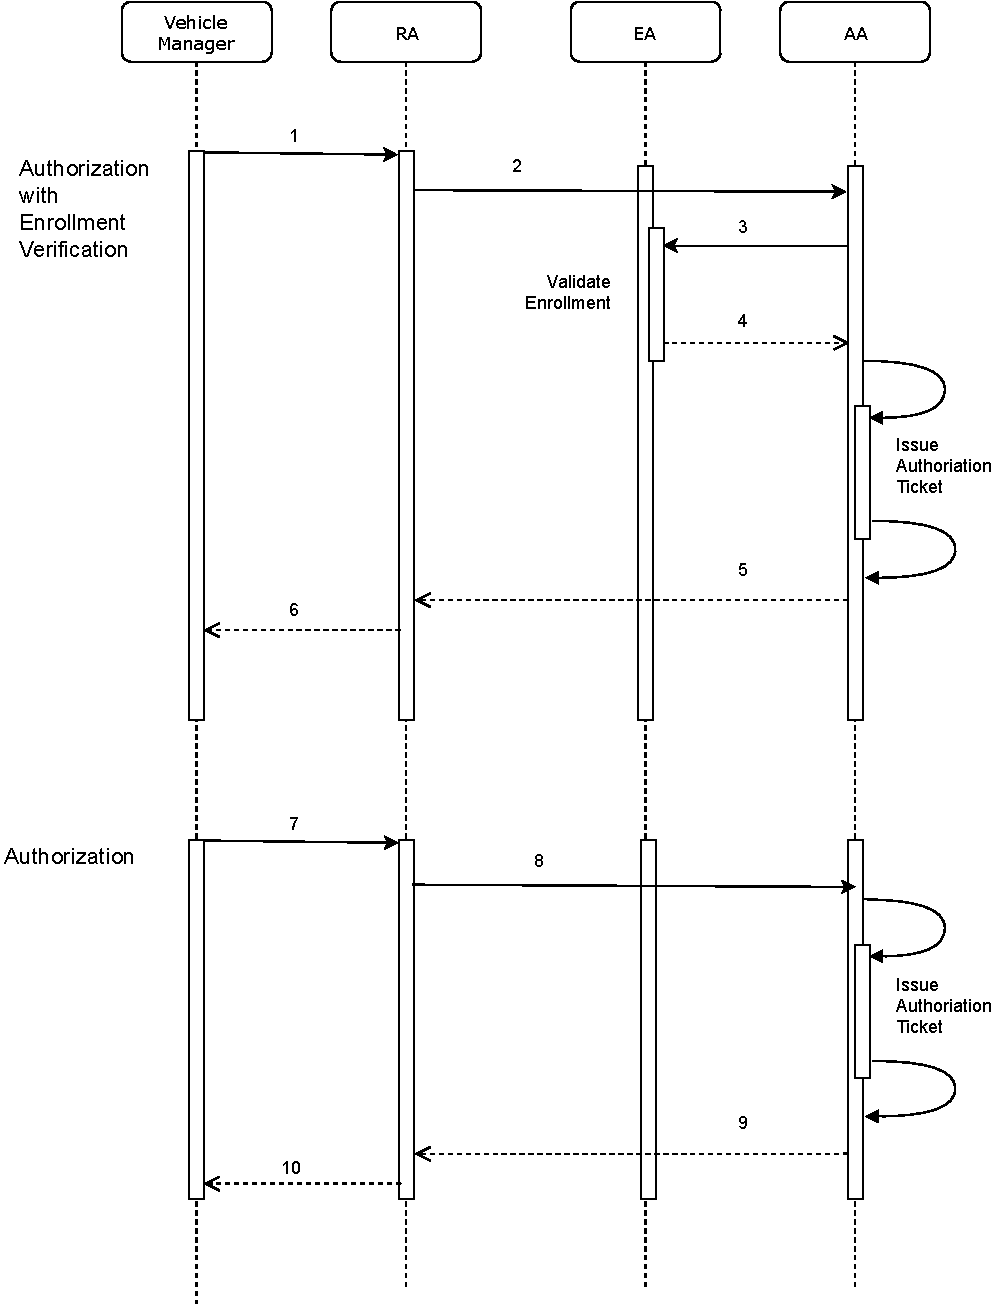
\includegraphics[width=0.8\textwidth]{Figures/protocolo_2}
	\caption{\label{fig:protocol_2}Vehicle authorization process flow.}
\end{figure} 

\subsubsection{Vehicle Authorization} \label{auth}
The last phase is the authorization which can be started by the enrolled vehicles. As the last phase, the security of this interaction is assured by the secure communication channel between the Vehicle Manager and PKI Manager, and by the application layer. Each time a vehicle requests one authorization ticket to an AA its enrollment must be verified. However, if such validation is performed by the AA the privacy of the vehicle would be compromised as the AA would have access to both the vehicle enrollment information (identity) and the pseudonym authorization ticket. To protect the vehicle's privacy, the enrollment validation is done by the EA which issued the vehicle's enrollment credential. Since a vehicle needs more than one authorization ticket, the consequence of this added privacy is the need to send more messages decreasing the performance of the vehicle authorization process as a whole. 

As we can see from Figure \ref{fig:protocol_2}, we have two flows from which a vehicle can request an authorization ticket. This enables us to leverage the RA in order to speed up the authorization process for each vehicle. The authorization process for a vehicle consists of multiple requests, if the vehicle is requesting the first authorization ticket the enrollment will be validated by the EA, otherwise the RA informs the AA that the vehicle's enrollment was previously validated. For the first authorization request, the vehicle starts by building the authorization request structure, such request contains all the information that the EA needs to validate the vehicle's enrollment status and that the AA needs in order to issue an authorization ticket. To ensure security and privacy in this type of communication, the vehicle's enrollment information such as its enrollment signature is encrypted to the EA and the authorization information encrypted to the AA. The vehicle sends message 1 containing the authorization request to the RA which knows how many requests the vehicle will perform during its authorization process. Message 2 shows the request being sent to the AA which decrypts it and sends the enrollment information to the EA in message 4. The EA decrypts its part of the request, validates the vehicle's enrollment signature, using the vehicle's enrollment credential (referenced by the request), and validates if such certificate is valid. If the verifications are in order, the EA sends message 4 which notifies the AA that the vehicle is authentic. The AA then issues the Authorization ticket, builds an authorization response structure which is signed, encrypted to the vehicle and sent to the RA within message 5 as a positive authorization.

At this point the RA knows that the vehicle is enrolled and that the authorization was successful, and is able to return the response to the vehicle in message 6. For the remaining requests the vehicle builds the authorization request and sends it to the RA as usual, as seen in message 7. The RA knows that the vehicle's enrollment has been validated for this authorization process and sends the request to the AA in message 8, the AA decrypts the requests, validates the authorization information, issues the authorization ticket, and returns the response to the RA in message 9. In the last step, message 10 shows the RA returning such request to the vehicle which stores the requested certificate. The same flow is repeated until the vehicle has all the authorization tickets for the time specified by the RA. 

\section{V2X Library}
As discussed before, one of the most basic concerns of this work is to implement a V2X ecosystem that is compatible with the most recent standardization efforts done by European organizations. In order to satisfy this requirement, the V2X library was implemented with ETSI’s standards in mind.
However, instead of blindly coding the information specified on the European standard we first searched for an already existing implementation. We found such a solution on the GitHub repository named C2C-Common \cite{c2c-common}, an open source Java package. However, upon closer inspection we noticed that C2C-common does not support the latest version of the European standard (1.3.2 at the time of this writing). In order to not reinvent the wheel, we decided to extend C2C-common by adding the necessary changes. In this section, we start by describing the detailed architecture of the library, then we take a look at the implementation of some of its most important data structures, and finalize by describing the services that our library provides. 

\subsection{Detailed Architecture}
The architecture of the V2X Library can be described as a layered structure, where at the highest level we can find the classes which allow the generation of the more specific data structures such as the EA, AA and Root CA certificates; vehicular authorization and enrollment certificates; and the V2X messages such as CAMs. As we go down a level the can find the more general substructures which the higher level structures depend. Finally, at the lower level we can find the classes which enable the transmission of such data structures in a cross-platform way.

As we can see from Figure \ref{fig:v2x_arch} the architecture of the V2X Library is divided in three layers. Starting at the layer 1 we have the super classes which are responsible to implement the Abstract Syntax Notation 1 (ASN.1) Canonical Octet Encoding Rules (COER) as used by the ETSI standard. The ASN.1 is a standard description language for defining data structures that can be serialized and deserialized in a cross-platform way. ASN.1 is closely coupled with a set of encoding rues (e.g. COER) which specify how to represent a data structure (e.g. an integer) in a series of bytes (serialization) and vice-versa (deserialization). At this level, we can find the most basic of COEREncodable structures such as sequence, enumeration, choice, etc. as well as their implementation of the encoding/decoding methods. Such structures will be part of the V2X certificates and messages according to the specification of ETSI. Because the definition of these structures and the respective encoding/decoding implementations depend only on the version of ITU-T X.696 standard \cite{coer_standard}, change on the C2C-common library at such a low level was not needed. In addition to the implementation of the COER structures, it is at this layer that the V2X has performs the most basic cryptographic operations. Such operations include the digest, signature and encryption of data and will be used exclusively by the layer 2 in order to build the data structures which require them. For example, certificates and V2X messages are always signed, and certificate requests are both signed and encrypted. 

Going up a level we can find the sub-classes of the more general COER structures, for example, the certificate which is a child of COERsequence. This means that a certificate is just a sequence of fields (i.e. base data structures such as the host name, issuer identifier, duration validity, signature, etc) and should be encoded/decoded as such. Because the certificate and message structures depend on the version of the ETSI standard, it was at this level that we introduced more changes to this library. 

Besides updating C2C-common, our contribution also included the addition of a new set of standardized messages, the request for vehicle certificates. Such messages are encrypted and signed to assure confidentiality and authentication on the certificate request and deliver. In our case, they are used by the vehicle manager and RA. The specification of this data structures can be found in the ETSI's Trust and Privacy Management standard \cite{etsi_privacy} and follow the same COER encoding rules. 

At the layer 3 we can find the generator classes that the library user needs to instantiate in order to generate certificates, V2X messages and certificate requests. The generator classes are responsible to implement the certificate profiles for the different subjects and the different types of V2X messages for the vehicles. In addition to the generators, this layer also provides to the user the higher level cryptographic operations such as the validation of a V2X message, certificate, generation of a new keypair, etc. In our case, the generator classes and the user cryptographic module will be used by interfaces present on the Vehicle Manager and PKI Manager. 

To assure that every data structure is correctly implemented unit tests were performed to test the serialization and deserialization of the objects.

\begin{figure}
	\centering
	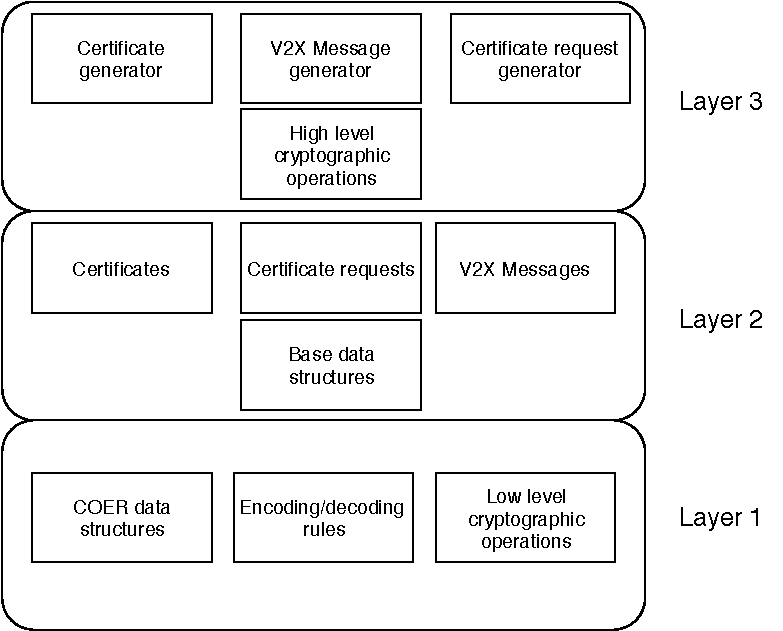
\includegraphics[width=0.8\textwidth]{Figures/v2xlib}
	\caption{\label{fig:v2x_arch} Layered structure of the V2X Library.}
\end{figure}

\subsection{The Data Structures}
We have seen how the library is organized, now we take a look at the implementation of the most important V2X structures. We start by describing the lower level COER structures, then we describe the higher level structurs such as the certificate requests.

\subsubsection{COER Structures}
Before we can understand the higher level data structures, we have to understand the lower level COER structures which are part of them and therefore are the base of this library. All implemented data structures derive from the same type, the \textit{COEREncodable}, which allows us say that each can be encoded or decoded according to the \textit{COER} rules. In terms of implementation, this is enforced by the \textit{COEREncodable} interface which declares two methods, one for encoding and the other for decoding. This interface provides us with a solid base, as any class that implements it is able to provide its own implementation of the two methods. The classes which implement this interface are one level higher than the base type, they are the \textit{COER} structures. In this Section we describe the implementation of the most complex of such structures, the \textit{COERSEquence} and \textit{COERSChoice}. To understand the relation between the classes, Figure \ref{fig:coer_structures} provides an UML classdiagram. 

\begin{figure}[t]
	\centering
	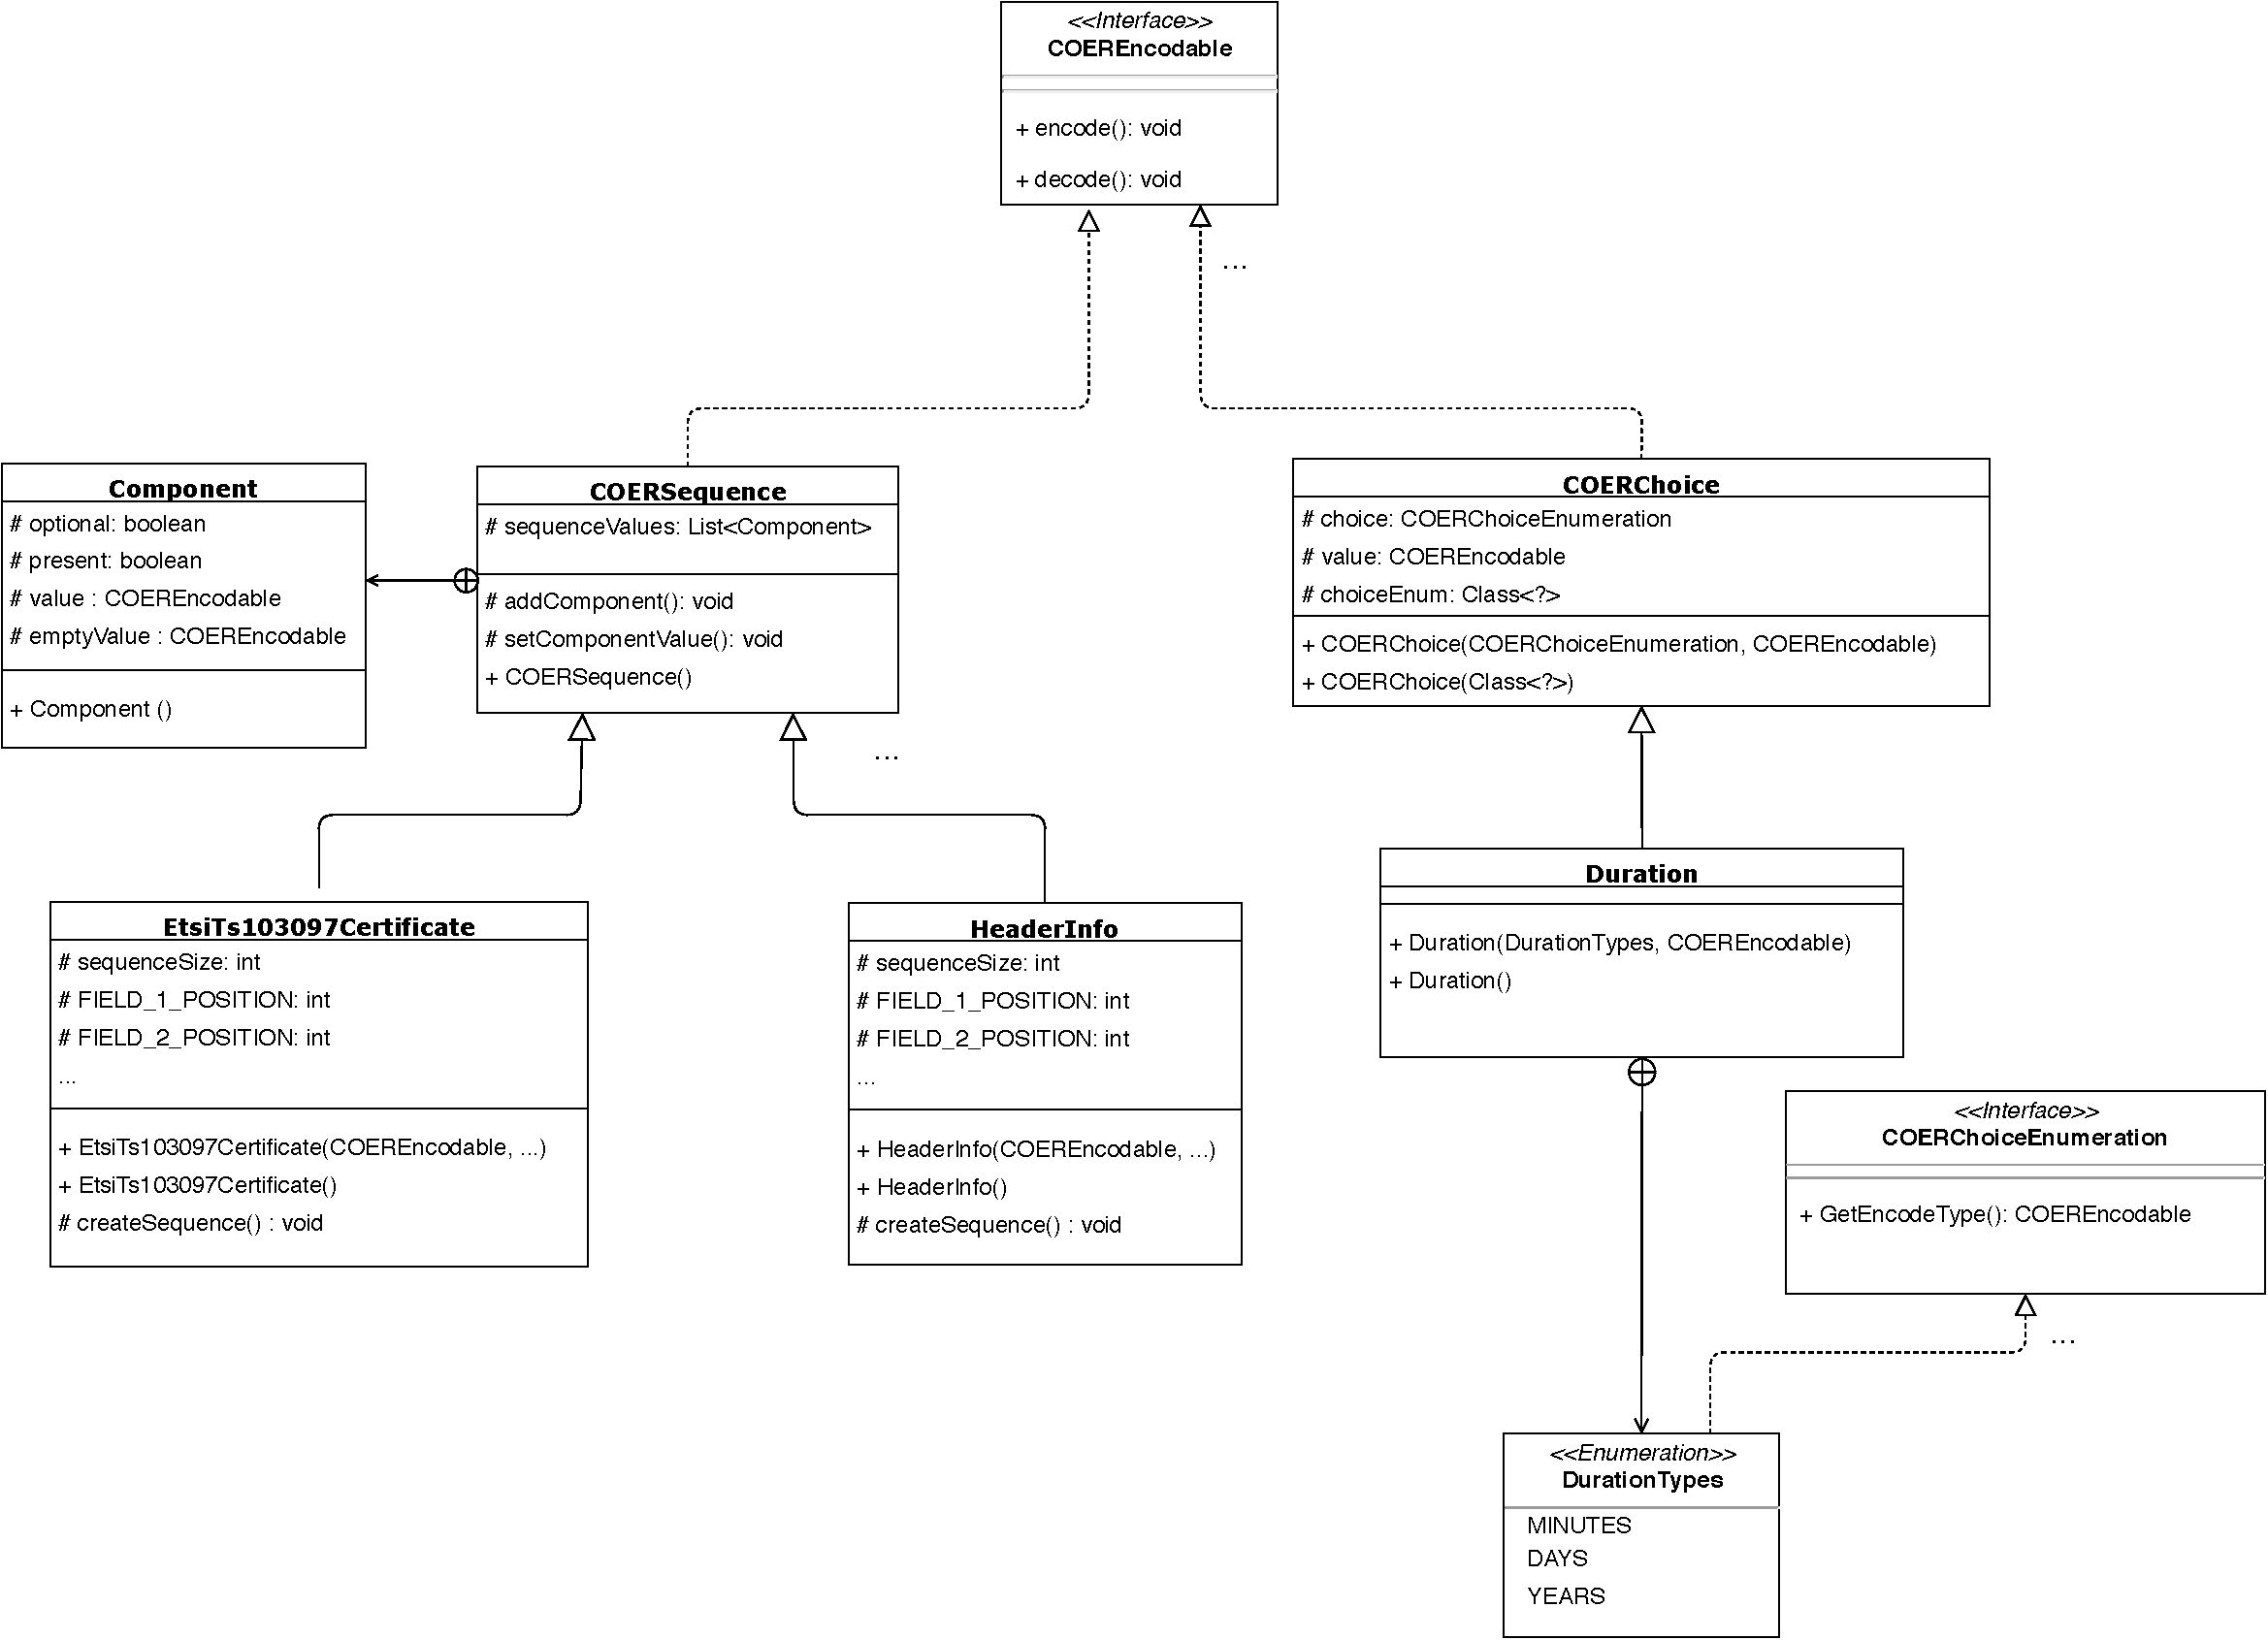
\includegraphics[width=1.1\textwidth]{Figures/coerstructures}
	\caption{\label{fig:coer_structures} Class diagram of the V2X {COER} structures.}
\end{figure}

\paragraph{COERSequence} The \textit{COERSequence} is a class which implements the encoding and decoding of a sequence of \textit{COEREncodable} elements. This class is very useful in the V2X Library as it allows us to combine a set of elements in a specific order to form a higher level data structure like a \textit{EtsiTs103097Certificate}. Generally speaking, the \textit{COERSequence} is a super class which provides the implementation of the \textit{encode} and \textit{decode} methods. Such class can be extended in child classes which can be seen as more specific types of \textit{COERSequence}, for example, the \textit{EtsiTs103097Certificate} which is an ordered sequence of certificate fields, and \textit{HeaderInfo} representing a specific sequence of header fields on a V2X message. Once an object of the sub class is instantiated it is possible to call the \textit{encode} or \textit{decode} methods to assure that the encoding rules are respected according to their definition on the super class. 

\begin{comment}
An object of a child class can be instantiated in two modes: for encoding or decoding a sequence. The general idea is that when an object of the subclass is created for encoding it initializes all attributes on the super class which are needed to encode it, making it possible to call the \textit{encode} method afterwards. When an object of the sub class is created for decoding it creates a placeholder object which then will be filled by the \textit{decode} method with a real values.
\end{comment}


In terms of implementation, the \textit{COERSequence} class represents an ordered sequence by having a list of \textit{Components} as a class attribute. A \textit{Component} is a helper class that represents a single component within the sequence. This class contains the to be encoded \textit{COEREncodable} value; a boolean variable representing if this value is optional; and an empty \textit{COEREncodable} object which indicates the value's type in the decoding logic. This list of components represents the \textit{COERSequence} and is initialized by the class's constructor which receives the sequence's size in the parameters. The other classes that extend the \textit{COERSequence} are able to interact with such list during the process encoding or decoding an object. 

Before a sequence can be encoded it must be first populated, the \textit{COERSequence} class provides two methods for this effect: the \textit{addComponent} and \textit{setComponentValue}. The first method has the responsibility of creating the frame of the sequence, which is relevant to the decoding process to indicate the specific component type, position in the sequence, and whether the component is optional. The second method can be posteriorly called to add the sequence values to the frame, completing the creation of the sequence. It is possible to add a \textit{null} value in the sequence when the value is optional and not present. To minimize usage errors, \textit{setComponentValue} always checks if the mandatory components are present.



\paragraph{COERSequence Encoding}
The encode process starts when creating a sub class of \textit{COERSequence} (e.g \textit{EtsiTs103097Certificate}) using its dedicated encoding constructor with the sequence values as parameters. Each sub class maintains its own frame information such as the sequence size, component order and optionality. Because of this, when an object of the sub class is created for encoding the constructor is able to initialize the list of \textit{Components} within the super class. This process is achieved in three steps: first the super constructor is called with the sequence size, then the \textit{addComponent} and \textit{setComponentValue} methods are called for each sequence element with the respective frame information and value. Once the sub class object is created, it is possible to encoded it by calling the \textit{encode} method. This method receives a \textit{DataOutputStream} in which the encoded bytes will be written to. The encoding of a \textit{COERSequence} consists of a preamble followed by the encoding of each sequence element. The preamble is a stream of bits which allows specifying the presence of the optional elements in the sequence. Each present element (not null) is then encoded with respect to its type (e.g COERInteger, COERString, Signature, etc) in the order that they appear in the sequence. 

\paragraph{COERSequence Decoding}
The decoding process is similar to the encoding. Instead of calling the encoding constructor we call the decoding constructor to create the frame of the sequence within the super class \textit{COERSequence}. This is achieved by the decoding constructor in two steps: calling the super constructor with the sequence size, and the \textit{addComponent} method for each sequence element with its type, order and optionality. The result is the list of \textit{Components} on the super class containing the frame of the sequence but no values. We now have a \textit{COERSequence} sub class which is instantiated to be part of the decoding process. To do so, we just need to call the \textit{encode} method with the \textit{DataInputStream} in which the encoded values will be read from. The process of decoding starts by reading the preamble to identify which of the optional values are present. The next step is to decode each present sequence value into their original object. This is done by iterating through each member of the empty list of \textit{Components} and decoding it according to its type (represented by the empty \textit{COEREncodable} value). The final step is to set the \textit{Component} value to the obtained object. When the decode process finishes, the sub class will have access to the complete sequence in the \textit{COERSequence's} class list attribute.


\paragraph{COERChoice}
The \textit{COERChoice} is a class that implements the encoding and decoding of a choice of \textit{COEREncodable} elements. This class is very useful in the V2X Library as it allows us to specify the choice of one element from a set of known \textit{COEREncodable} values. Some applications include: the type of time duration on a certificate's validity (years, days etc.), the certificate's issuer identifier (self signed or digest of the issuer's certificate), and many others. 

Like the \textit{COERSequence} and all other COER classes, the \textit{COERChoice} is a super class which provides the implementation of the \textit{encode} and \textit{decode} methods. The process of encoding or decoding a choice starts when creating a child of the \textit{COERChoice} (e.g. \textit{Duration}) using the dedicated constructors. 


The objective of the encoding constructor is to initialize all the attributes on the super class (\textit{COERChoice}) needed for encoding. Such attributes include the choice and its value. To implement this, all sub classes contain a Java enumeration listing the possible choices for its type, for example \textit{Duration} contains an enumeration listing the possible types of time duration (microseconds, seconds, days and years). With this enumeration it is possible to instantiate a sub class object by calling the encoding constructor and passing an item which represents the choice and its corresponding \textit{COEREncodable} value. 

To uniformize the type of these enumerations through all the \textit{COERChoice's} sub classes, they implement the same \textit{COERChoiceEnumeration} interface. This enables the encoding constructor of the sub class to call the corresponding constructor on the \textit{COERChoice} passing the \textit{COERChoiceEnumeration} item and the value. An example of this interaction would be creating an object of \textit{Duration} with the \textit{COERChoiceEnumeration} item of \textit{YEARS} and the value of 4, representing a duration of four years. In this case the \textit{Duration} class encapsulates the value in to a \textit{Uint16} structure, an unsigned 16 bit \textit{COEREncodable} integer, and calls the \textit{COERChoice} encoding contrustor with the choice of duration (time unit) and the value. Thus, initializing the super class attribues for encoding and concluding the creation of the \textit{Duration} object. 


\paragraph{COERChoice Encoding}
To encode the created sub class object we simply need to call the \textit{encode} method, the implementation of this method exists in the super class because it is the same for all types which extend the base type of \textit{COERChoice}. In terms of implementation, the \textit{encode} method works with the attributes of the choice (\textit{COERChoiceEnumeration}) and value (\textit{COEREncodable}). The encoding consists in the creation of a tag followed by the encoding of the \textit{COEREncodable} value. \textit{COERTag} allow the decoder to know the specific choice that the value belongs to, as it contains the position of the choice within its \textit{COERChoiceEnumeration}. This stream of bytes is enabled by the \textit{getOrdinal} method which is implemented within all \textit{COERChoiceEnumerations}, thus allowing the \textit{COERChoice} class to call it using its choice attribute. The \textit{encode} method then creates and encodes a \textit{COERTag} object with the ordinal value, encodes the \textit{COEREncodable} value (in the class value attribute), and finally appends it to the tag. The result is a stream of bytes representing the choice and the value.

\paragraph{COERChoice Decoding}
The process of decoding a sub class of \textit{COERChoice} is similar to the encoding, as it starts by creating an object of the sub class but calling its decoding constructor. Such method will initialize the choice attribute on the super class so that the value can be filled by the decoding process. This is achieved by calling the corresponding constructor on the \textit{COERChoice} class with the main type of the \textit{COERChoiceEnumeration}. For example, in the case of the \textit{Duration} class is the \textit{DurationTypes} enumeration which implements the \textit{COERChoiceEnumeration} interface. This will initialize the \textit{choiceEnum} attribute on the super class which is needed for the decoding process. Once the empty object is created (i.e. without the value), the \textit{decode} method can be called. Such method will first decode the \textit{COERTag} to get the specific choice from its \textit{choiceEnum} attribute. With the choice it is possible to get the \textit{COEREncodable} value associated to it, we just need to know its main type. This is achieved by the \textit{getEncodableType} method which is implemented within the \textit{COERChoiceEnumerations}, thus enabling the \textit{decode} method to use it on the recently discovered choice attribute. This method contains a switch that given the choice will return its intended main type. For example, in the \textit{DurationTypes} enumeration it will return an empty object of \textit{Uint16} since this is the type that represents the number of years, minutes, seconds, etc in a time duration. At this point the \textit{decode} method knows all the pieces to the puzzle and is able to decode the value by calling the \textit{decode} method for its main type. The application of this method will update the choice and value attributes of the \textit{COERChoice}, thus concluding the decoding. 


\subsubsection{Certificate Requests} \label{requests}
Besides updating the implementation of the certificates, V2X messages and all other data structures which they depend on, we had to implement the requests for vehicle certificates and their corresponding response. The specification for these data structures can be found on the ETSI's Trust and Privacy Management standard \cite{etsi_privacy} and they depend on the same \textit{COEREncodable} data structures as the V2X messages. 


\paragraph{Enrollment Request}
The first message that we implemented was the \textit{EnrollmentRequest} shown in Figure \ref{fig:enrollment_request}. This request contains two signatures and is encrypted to ensure the confidentiality, integrity and non-repudiation of the vehicle's important information such as the vehicle id, requested certificate attributes and the public verification which will be certified.

The request for an enrollment certificate is sent by the vehicles to an EA. In order to protect the privacy of the vehicles by hiding the vehicle's enrollment data such as ITS identifier this message will be encrypted with a symmetric key that is to be shared with the recipient EA. In terms of implementation, this message is an \textit{EncryptedData} structure which is a sequence that contains two elements: the recipient information and the ciphertext. The recipient information is the element that allows us to share the encryption symmetric key with the EA. This structure is implemented as a \textit{PKRecipientInfo} (Public key recipient information) containing the hash of the certificate that belongs to the recipient EA (\textit{recipientId}), and the 128 bit AES key encrypted with ECIES using the encryption public key of the recipient EA. The symmetric key is shared with the EA for of performance reasons, since encrypting large amounts of data with symmetric cryptography is faster than using symmetric cryptography. For interoperability reasons, the encryption algorithms used are the ones approved by the standard. The ciphertext is the request's outer signature structure.

The outer signature exists to prove that the requesting vehicle has possession of the canonical keypair which was attributed to it when it was manufactured or the keypair of a current valid enrollment certificate. This allows the EA to trust that the origin of this request is an authentic vehicle, assuming that such key pair was securely stored by the vehicle's OBU. In terms of implementation, the signature is contained in a \textit{SignedData} structure which is sequence that also contains fields relevant to the signature's validation as well as the signed data. Specifically, this structure contains: the id of the hash algorithm used, signed data, signer information, and the signature itself. The signature over the to be signed can be calculated by two district ways depending on the vehicle's enrollment state: if this is the first enrollment request, the signature should be done with the vehicle's private canonical key; else it should be done with the private key of the currently valid enrollment certificate. To indicate the signature method, the field signer identifier is a \textit{COERChoice} which contains the hash of the enrollment credential in the case re-enrollment or empty otherwise. The data protected by the signature (signed data) is a sequence that contains a header and payload. The header is the data structure which contains information needed for the validation of the outer signature, it contains the \textit{Provider Service Identifier} PSID and the signature generation time. The PSID is a \textit{COERInteger} which identifies this message as a secured certificate request as assigned in the ETSI TS 102 965 standard \cite{etsi_PSID}. The payload of the outer signature contains the request's inner signature.

While the outer signature serves to prove the identity of the vehicle, the inner signature serves to prove that the requesting vehicles has position of the verification key pair which will be part of its enrollment certificate. I terms of implementation, the inner signature is very similar to the outer signature as it depends on the same sub structures. The only difference is that this signature is done using the vehicle's private verification key corresponding to the public key to be sent by this request. Therefore, the signer information field is always empty, indication that this is a self signed signature. The payload contains the data relevant to the emission of the enrollment certificate, this data is wrapped in a \textit{InnerECRequest} structure which is as a sequence containing: the vehicle's identifier, the version of the certificate standard, the public verification key, and the requested subject attributes. The requested attributes are the desired enrollment certificate attributes and contain data such as the enrollment validity period, region, desired application permissions, and the certificate subject name. 

\begin{figure}
	\centering
	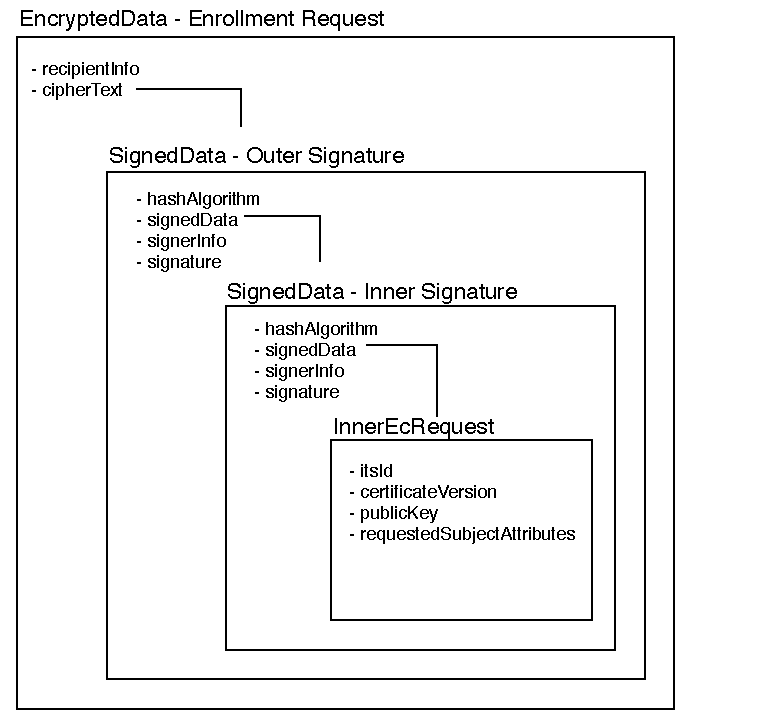
\includegraphics[width=0.8\textwidth]{Figures/enrollmentrequest}
	\caption{\label{fig:enrollment_request}Enrollment request message.}
\end{figure}

\paragraph{Enrollment Response}
The second request that we implemented was the \textit{EnrollmentResponse} shown in Figure \ref{fig:enrollment_response}. This message will be sent by the EA to the vehicle in response to its enrollment request. To protect the vehicle's privacy and securely deliver the enrollmnet certificate this request is signed and then encrypted. The request is encrypted using the symmetric key which was shared by the vehicle through the enrollment request. To indicate this, the recipient information is implemented as a \textit{PreSharedKeyRecipientInfo} structure which contains the hash of the AES key. The ciphertext of the encrypted data contains the enrollment response signature, which is done using the private key that is paired with the EA certificate's verification public key. This signature allows the vehicle to validate that the response originated from the correct EA. The signature protects the \textit{InnerECResponse} which contains the original request's hash value, a response code, and possibly the requested enrollment certificate. The hash value allows the vehicle to map this response to the original request by calculating and comparing its hash value. The response code indicates whether the request was successful or not. 

There are many possible ways which can cause the EA to decline the enrollment request, for example, if it can't parse the request, can't' decrypt, the EA is not the recipient, invalid vehicle signatures, denied permissions, etc. To inform the vehicle of the problem, \textit{EnrollmentResonseCode} is a COEREnumeration which encodes the possible outcomes of the EA's enrollment validation. Only in the positive case the \textit{InnerECResponse} provides the enrollment certificate. 

\begin{figure}
	\centering
	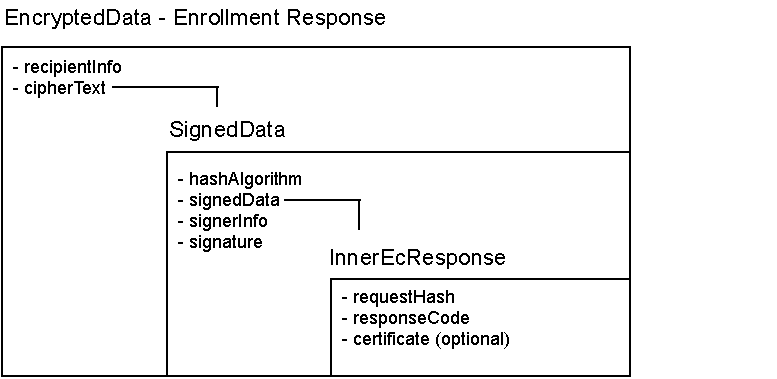
\includegraphics[width=0.8\textwidth]{Figures/enrollmentresponse}
	\caption{\label{fig:enrollment_response}Enrollment response message.}
\end{figure}

\paragraph{Authorization Request}
After we implemented the enrollment request and response we implemented the \textit{AuthorizationRequest} shown in Figure \ref{fig:authorization_request} since it depends on the vehicle's enrollment certificate. The authorization request is sent by enrolled vehicles to an AA which sends the enrollment certificate to the EA for vehicle enrollment validation. Since the authorization request includes the vehicle's enrollment certificate it introduces privacy concerns regarding the ability of the AA to link the enrollment certificate to the issued authorization tickets. To protect the vehicle's privacy the authorization request can be divided in two parts: the part which is encrypted to the AA and the part which is encrypted to the EA.

The process of encrypting the request for the AA is similar to the one used in the enrollment request since we are encrypting data to a certificate recipient. The authorization request is an \textit{EncryptedData} structure containing the recipient information and the ciphertext. While the recipient information contains the shared symmetric key which decrypts the request. The encrypted data is a \textit{SignedData} structure which ensures the AA that the vehicle is in possession of the verification key pair which will be certified by the authorization ticket. The signed data within this structure is the \textit{InnerATRequest} which contains the information that the AA needs to issue the authorization ticket and the information that the EA needs to validate the vehicle's enrollment. The \textit{InnerATRequest} is a sequence that contains: the verification public key, a \textit{ecSignature}, and \textit{sharedATRequest} structures. The \textit{sharedATRequest} is a structure which is to be shared between the AA and EA, it contains information that needs to be validated by both authorities in order to issue the authorizatio ticket. This structure contains the \textit{eaId}, allowing the AA to know which was the EA that enrolled the requesting vehicle; and the requested subject attributes which will be validated by the authorities. The \textit{ecSignature} contais the vehicle's enrollment credential signature, which is the part of the authorization request encrypted to the EA to ensure privacy in the enrollment validation. The ciphertext contains the signature computed with the private key corresponding to the enrollment credential of the vehicle. This mechanism allows the EA alone to decipher its part of the request and validate the vehicle's enrollment. To specify to the EA which enrollment credential was responsible for the signature, the field signder identifier contains the hashed vehicle's enrollment certificate. The signed data contains the hash of the previous \textit{sharedATRequest} since this structure is to be seen by both the EA and AA, therefore it can not be directly included in the encrypted \textit{ecSignature} structure. This external payload mechanism on \textit{ecSignature} allows it to ensure the integrity and non-repudiation of the \textit{sharedATRequest} while hiding vehicle's enrollment credential to the AA and still allowing it read the \textit{sharedATRequest}. 

\begin{figure}
	\centering
	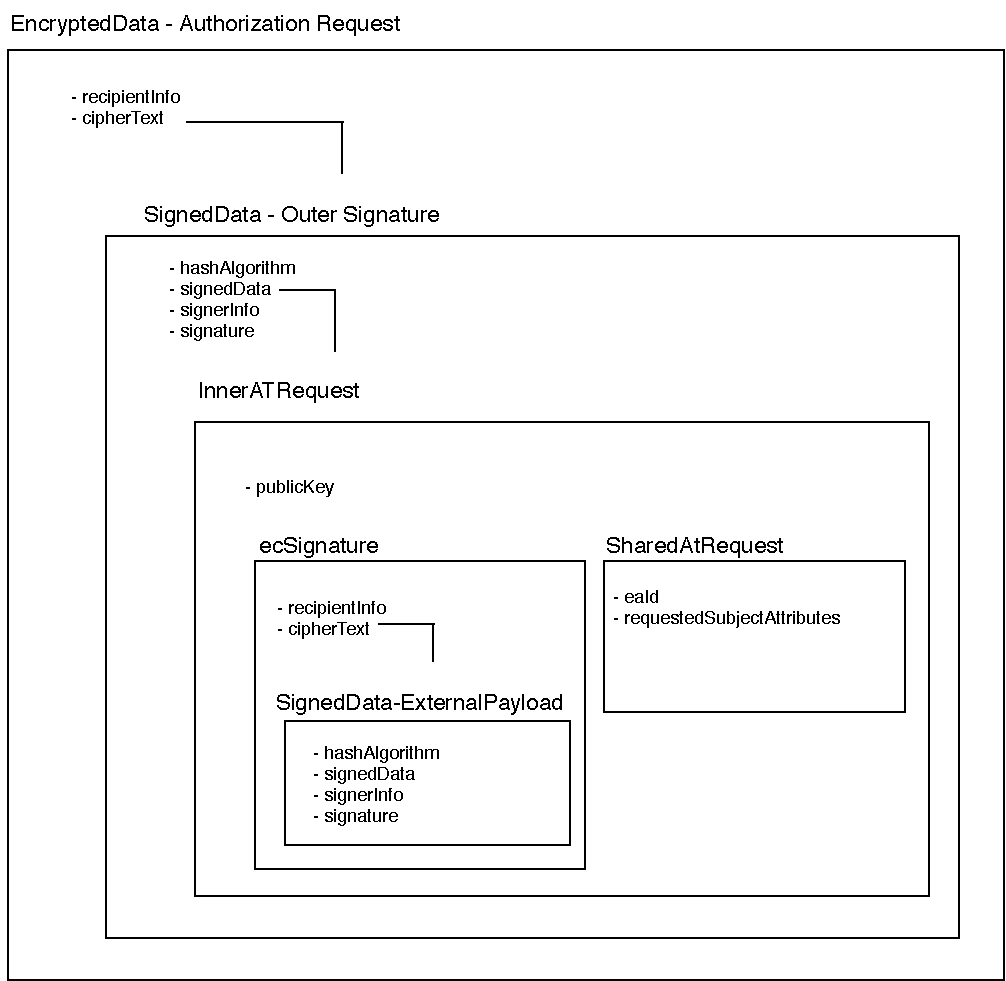
\includegraphics[width=0.9\textwidth]{Figures/authorizationrequest}
	\caption{\label{fig:authorization_request}Authorization request message.}
\end{figure}

\paragraph{Authorization Validation Request and Response}
These request/response messages are the intermediate step in the vehicle's request for an AT. To validate the vehicle's enrollment an \textit{AuthorizationValidationRequest} is constructed by the AA and sent to the EA. This structure contains elements from the Authorization request which was sent by the vehicle to the AA. Specifically, the \textit{ecSignature} and \textit{sharedATRequest}. The response is sent by the EA to the AA and contains the response code which will determine whether the AA is allowed to issue the AT or not. 

In terms of implementation the response is a \textit{AuthorizationValidationResponse} structure which is a sequence that contains the request hash, response code and the confirmed subject attributes. The request hash is SHA-256 digest of the \textit{AuthorizationValidationRequest} which will allow the AA to associate this response to its original validation request. The response code indicating the result of the EA's internal vehicle enrollment validation. In the positive case, the field confirmed subject attributes contains the subject attributes that the EA wishes to confirm; in the case that the EA denies the vehicle's enrollment the response code contains the reason, and the confirmed subject attributes is empty.

\paragraph{Authorization Response}
The \textit{AuthorizationResponse} shown in Figure \ref{fig:authorization_response} is the last message to be sent in the vehicle's authorization request. This message is sent by the AA to the vehicle and may contain the requested AT. To protect this response the message is signed by the AA and then encrypted such that only the original vehicle is able to decrypt. The encryption is similar to the method used in the enrollment response since a symmetric encryption key was previously shared by the vehicle with the AA in the Authorization request. The cipher text is a \textit{SignedData} structure which contains a signature done with the AA's private key that corresponds to its authority certificate. The signed data is the \textit{authorizationResponse} which contains: the request hash, allowing the vehicle to associate the AT request; the response code, which indicates the result of the authorization process; and the optional AT that is only present in the successful authorization case.
 
\begin{figure}
	\centering
	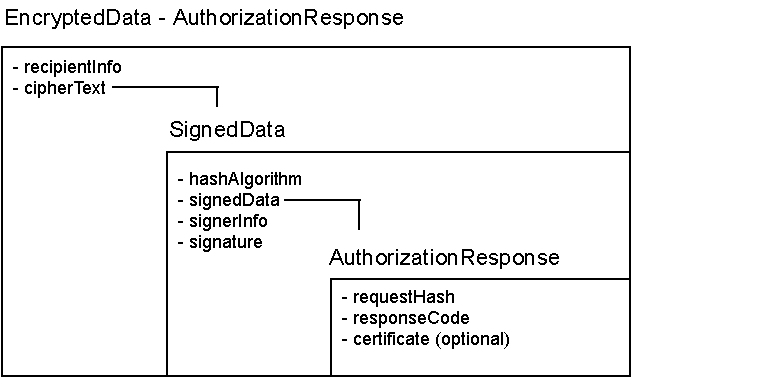
\includegraphics[width=0.8\textwidth]{Figures/authorizationresponse}
	\caption{\label{fig:authorization_response}Authorization response message.}
\end{figure}


\subsection{The Cryptographic Tools}
When privacy and security are requirements of a system, the use of cryptographic tools is essential. Such tools allow us to keep the information confidential thorough communication, to verify its integrity, freshness and authenticity.

The process of providing the secured data structures to the other system components implies that it is this library’s responsibility to perform the needed cryptographic operations in order to generate them. To facilitate interoperability between other potential systems, it is essential that such operations are performed according to the algorithms described in the latest version of the IEEE 1609.2 standard, which are also used by ETSI 103 097.

At a low level, the V2X Library uses Bouncy Castle as a security provider for all of its cryptogtaphic operations. Such API pvoides us with the implementation of the cryptogaphic algorithms allwoing us to abstact from their complex implementation details when performing cryptographic operations.
The V2X library contains within its functionalities the following cryptographic operations: 

\begin{itemize}
	\item The generation of symmetric and asymmetric keys. This operation must be called providing one of the supported key generation algorithms.
	\item The signing of data. This operation must be called providing a supported elliptic curve signing algorithm, the data to be signed, the signing certificate, and the signing private key. The result is a \textit{Signature} structure as defined in the European standard. 
	
	\item Verification of a digital signature. This operation must be called providing the data to be verified, the \textit{Signature} data structure, and the signing certificate with the correspondent certification chain. This function returns a Boolean value corresponding to the validation result. 
	
	\item Asymmetric encryption of symmetric key. Encrypting large amounts of data with asymmetric keys is inefficient, this should be done using symmetric keys. However, in order to decrypt a symmetric encrypted message, its recipient must have access to the same secret key (i.e. symmetric key) which encrypted the message. This operation exists to assure confidentiality in the process of sharing a secret key with a specific recipient. It should be called providing the secret key that will be encrypted, a supported elliptic curve encryption algorithm, and the public key of the recipient. 
	
	\item Asymmetric decryption of symmetric key. This operation must be called providing the encrypted symmetric key, the recipients private key and the elliptic curve decryption algorithm.
	
	\item Symmetric Encryption of data. This operation should be used to encrypt data with the \textit{AES CCM mode} algorithm, to call it we need to specify the data to be encrypted, the secret key and a nonce. The last parameter is to be used as input to the initialization vector for the encryption algorithm.
	 
	\item Symmetric Decryption of data. This operation must be called providing the encrypted data, and the decryption key and nonce which was originally used to encrypt the data. 

	
\end{itemize}

All of these operations are available at the Crypto Manager which was implemented as the default cryptographic module of V2X Library. It is also possible to extend the Crypto Manager in the future by adding new operations or support for new algorithms.


\section{PKI Manager}
Certificate issuing is an essential part of this work, however due to time constraints we were not able to extend mPKI. Our solution to this problem was to create the PKI Manager, a web application that functions as a demo PKI. 

The PKI Manager contains a backoffice which was implemented with the sole purpose of demonstrating the creation of vehicular certificates. However, it is much more limited comparing to mPKI. In the PKI Manager all the cryptographic operations related to the generation of keys, certificates and messages are done using software (V2X Library). 

Such operations share the processing resources with the machine which the PKI Manager is deployed, which can cause the entire machine to slow down and decrease the performance of the PKI Manager. In terms of security, these operations are only secure as the rest of the machine. A single security flaw in the operating system can compromise the security provided by the software encryption. In addition to the constraints in performance and security, the PKI Manager is also limited in terms of functionality. Although it provides the most basic vehicular PKI operations such as the enrollment, re-enrollment and authorization of vehicles it does not support the revocation of the certificates which belong to the end entities and CAs though a CRL mechanism. In this section, we describe the application, the technologies adopted, the features that it provides, and our implementation decisions.

\subsection{The Technology}
The PKI Manager is a web application implemented using the Spring Boot framework. This framework produces a stand-alone application and aims to reduce the time spent configuring it. This is achieved automatically by Spring based on the dependencies added to the project. For example, if we add a dependency that relates to a database, Spring will attempt to auto configure the application for database access.

These applications run on an embedded container, which simplifies the deployment process of the web application. We simply need to press the “start button” and access the application at the address indicated by \textit{http://localhost:8081/}. This is done by Spring, because we added the spring-boot-starter-web dependency it pulls the spring-boot-starter-tomcat automatically which in turn starts Apache’s Tomcat Web Server when we run the main method.

Our web application is organized as a Spring Web MVC application, this framework is a module of Spring that specializes in aiding the development of web applications. It provides all the functionalities needed to receive HTTP requests, delegate their processing to other components, and finally, build a response. MVC is an acronym for model, view and controller each name represents a fundamental part of a Spring Web MVC application. In order to understand each part, I will describe the basic flow of an HTTP request from the point of view of the Spring MVC.

When we access an URL in the browser that sends an HTTP request to our server, for example our \textit{http://localhost:8081/}, the framework will try to find a class that is responsible to deal with such request, delivering to it the data that originated from the bowser. This class is an application controller. The controller then passes the data to a model, which executes the necessary business logic such as validation, calculations or database access. The result of the operations is returned to the controller, which in turn returns the name of the view along with the data needed to render the web page. Finally, the framework tries to find the specific view that is responsible to process such data into an HTML page and returns it to the browser. 

In regard to our application's identity management and user authentication we decided to use Spring Security since it is also a module of Spring. By using a configuration file, we can limit the web pages which the users and administrators can access while authenticated. This feature allows us to protect services and information from unauthenticated parties. The PKI Manager authentication is done using the usual username and password method. In this approach, the server stores the username and the hashed value of the password in its database. In addition to storing user credentials, the database also stores the role of each user allowing us to differentiate the privileges for the different types of users (regular user or admin). 

\subsection{The Database}
One of the concerns that we had when creating the PKI Manager was the persistence of the PKI information. We decided that even though this PKI exists for demonstration purposes, it would be important to store it in a non-volatile way. This decision allows us to keep consistency of the PKI even if the server crashes/restarts. In this section we describe the data access layer of the PKI manager, we start by introducing the technologies adopted, then we take a look at the design of the database. 

\paragraph{The database technology}
The database service is provided by PostgreSQL, a relational database management system. A database server runs locally, to which our application connects at the start of its execution.

The database access is provided by another of Spring's modules, the Spring Data JPA. This framework aims to simplify the data access layer of the applications by reducing the code needed for its implementation. To do so it relies on the entities and repositories. The entities are classes which correspond to tables in a database and are created with the help of the Spring annotations. It is through these annotations that we can specify the name of the table, its columns, primary keys, the relations between tables, etc. While the JPA entities allow us to shape the diagram of the database, the repositories provide us with a way to interact with it using queries. To be precise, these repositories are divided in two parts, the Repository and the Repository interface. The Repository is a class implemented by Spring, it has direct access to the database and queries it. The Repository interface is an abstraction of the Repository in which the developer can add methods in order to specify the supported queries. This can be done in different ways, for example, it is possible to create a query from the method's name or using Spring annotation. In our case, we used the first method for the more simple queries, and provided Spring annotation containing a native SQL query to support the most complex of the database queries. 

\paragraph{The database design}
To provide persistence with regard to the PKI Manager, we designed a database which keeps the information about the PKI entities and the operations of the PKI Manager. To minimize redundant data and facilitate finding information, we introduced relations between these PKI entities naturally. figure \ref{fig:database_diagram} shows the entities that we took into account, their characteristics and relations.


\begin{figure}
	\centering
	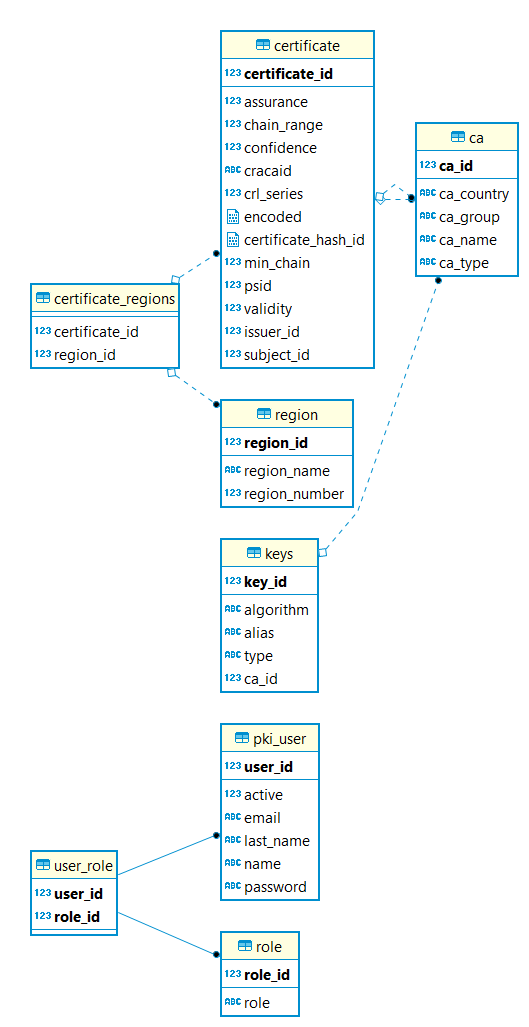
\includegraphics[width=0.8\textwidth]{Figures/db_diagram}
	\caption{\label{fig:database_diagram}Database entity relation diagram.}
\end{figure}

As we can see from the Figure, the database stores in its tables information to support the user authentication and management of the vehicular PKI. Regarding the PKI information, it has a table for the CAs, keys, certificates and regions. 

The \textit{ca} table contains generic CA information such the CA type (Root, AA, EA), group (Root CA or Sub CA), name, and country. It is possible for a CA to have one or more keys associated, this is expressed by the one-to-many relation between the \textit{ca} and \text{keys} tables. Regarding the relations between CAs and certificates, we assumed two occurrences: A CA can be subject of a single certificate and the issuer of one or more certificates. These relations are expressed by the one-to-one and one-to-many relation between the \textit{ca} and \text{certificate} tables.

The \textit{keys} table contains generic Key information but not the key itself, this is because the key is stored in a keystore. We only use this table to store information needed to locate the key in the keystore and view its characteristic, such as the alias, type of the key (encryption or signature), the algorithm. The foreign key \textit{ca\_id}, allows us to know which CA a specific key belongs to. 

Because currently there is not a keystore that supports the storage of this type of CA certificates, we decided to store them in the database. The \textit{certificates} table stores all the information that we need to pass to the V2X library in order to generate CA certificates. The foreign keys \text{subject\_id} and \textit{issuer\_id} allow us to know which CA is the subject and issuer of a specific certificate. 


\subsection{The Backoffice}
The PKI Manager is accessible through the browser only by system administrators. This backoffice application uses the V2X Library and through its services provides a GUI where administrators can visually create and configure a demo vehicular PKI. In this section we describe the functionalities and implementation details of the PKI Manager.

Upon logging in, the administrator will have the option of managing the CAs, keys, certificates, or viewing the PKI dashboard. These operations can be chosen from the index page, each having a dedicated web page. Performing a PKI operation updates the application dashboard, shown in Figure \ref{fig:manager10}, allowing the user to understand the state of the PKI. Specifically, whether the PKI has the necessary CAs and if each is ready to issue certificates. On the ramining of this section we take a look at the steps which an admin user has to take in order to create a PKI using our backoffice application.

\begin{figure}
	\centering
	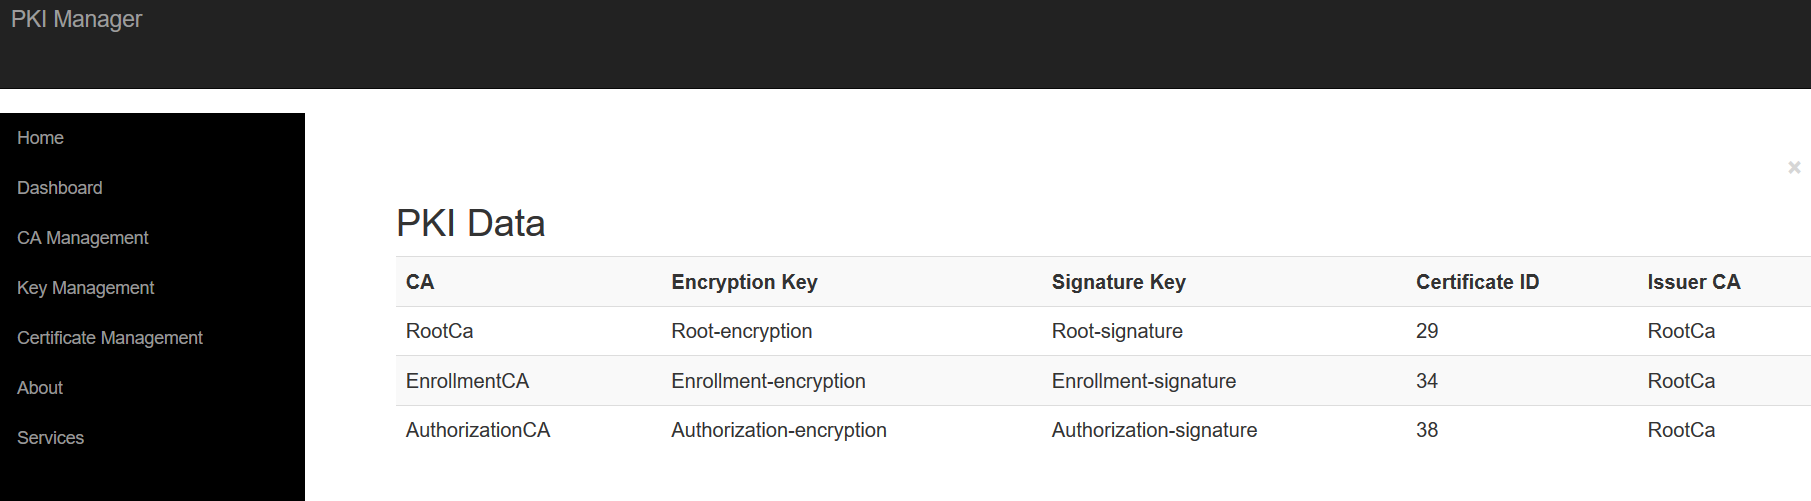
\includegraphics[width=0.8\textwidth]{Figures/manager10}
	\caption{\label{fig:manager10} Data of the created PKI}
\end{figure}

\paragraph{CA Management}
The first operation that should be done to have a functional PKI is the management of the PKI CAs. In this page, the user has the option of creating a CA by clicking a button. Performing this action displays the submit form shown in Figure \ref{fig:manager1}. In this form the user can specify the name, country and type of CA. The last is a drop down menu which shows the already defined CA types of Root, Enrollment and Authorization. When this form is submitted, this page's Spring MVC controller at the server-side will handle the POST request by storing the CA information on the database. To be precise, our controller calls the \textit{caManagementService} which performs the bussiness logic such as validation of the inputed information, then the service calls the \text{caRepository} that stores the information. When this logic is completed, the controller will redirect the browser to same CA management page, which makes it perform a GET request. The GET controller for this page will then handle such HTTP request by getting all the existing CAs from the database, returning them along with the requested web page to the browser. With this information it is possible to display the existing CAs as we can see from Figure \ref{fig:manager1}, updating the table each time we get the CA management page. 

\begin{figure}
	\centering
	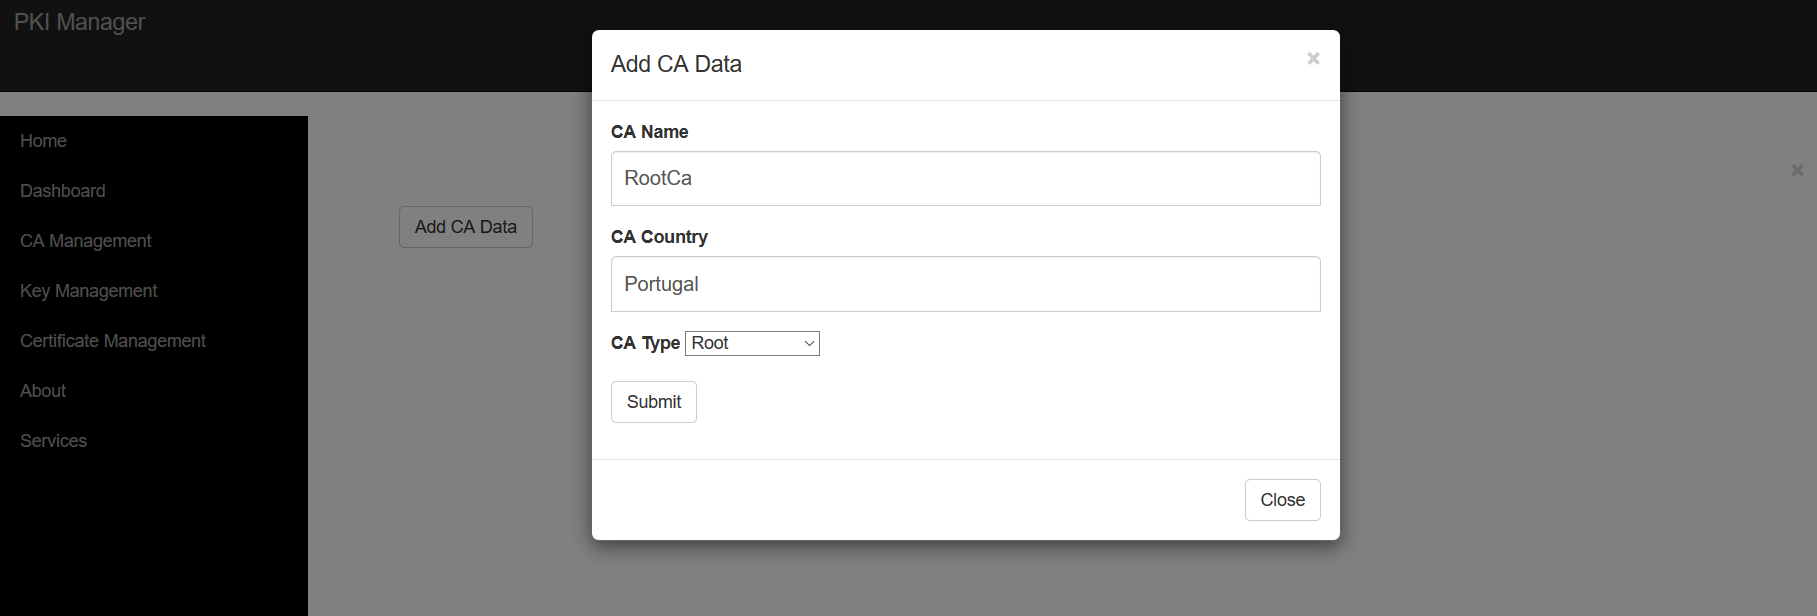
\includegraphics[width=0.8\textwidth]{Figures/manager1}
	\caption{\label{fig:manager1}From to add a new CA.}
\end{figure}

\begin{figure}
	\centering
	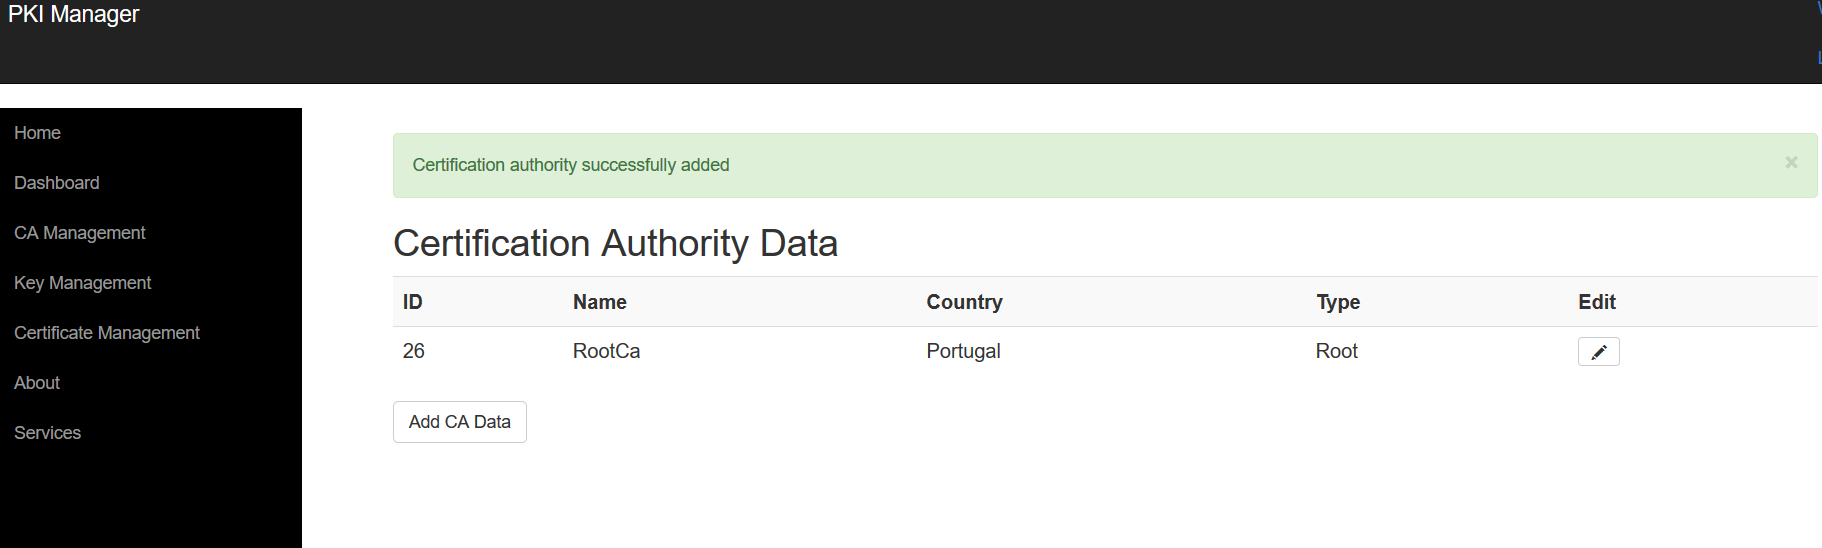
\includegraphics[width=0.8\textwidth]{Figures/manager2}
	\caption{\label{fig:manager2}Certification authority table.}
\end{figure}


The same logic is done for all the other operations, for each operation we have a spring controller which implements end-points that will handle HTTP GET and POST requests. The GET end-point has the responsibility of returning to the browser the web page with all the information needed to perform the operation. The POST end-point has the responsibility of generating resources (web pages, database information, services, etc.) on the server-side in respect to the information sent by the browser.

\paragraph{Key Management}
After creating a CA, the next step is to generate its signing and encryption keypairs. Once on the Key Management page, the user is able to do so by clicking a button. This button opens a form where the key alias, algorithm and owener CA can be chosen, as we can see in Figure \ref{fig:manager3} . In terms of constraints for these inputs, the alias must be unique, the user must select one of the provided encryption or signing algorithms, and one of the created CAs as the owner of the keypair. Being that these selectable values are loaded by the server in the browser when it requests this page. Submitting the form will send a POST request to our server, which will generate the key given the algorithm and store it with respect to the owner CA. The generation of the keypair is done using V2X Library interface which allows the PKI Manager to access the services of this library. The storage of the keypair is done regarding two aspects, the generated keypair and its information. The keypair itself is stored on a keystore file which is loaded into our server when its execution starts. The keystore data which is inputted by the user at the client-side is stored on the database. With this method it is possible to quickly search for a key in our database using its information and then find its value on the keystore providing the alias. Upon finishing these operations, the server will refresh the Key Management page, updating the existing keys table with the new entry.

\begin{figure}
	\centering
	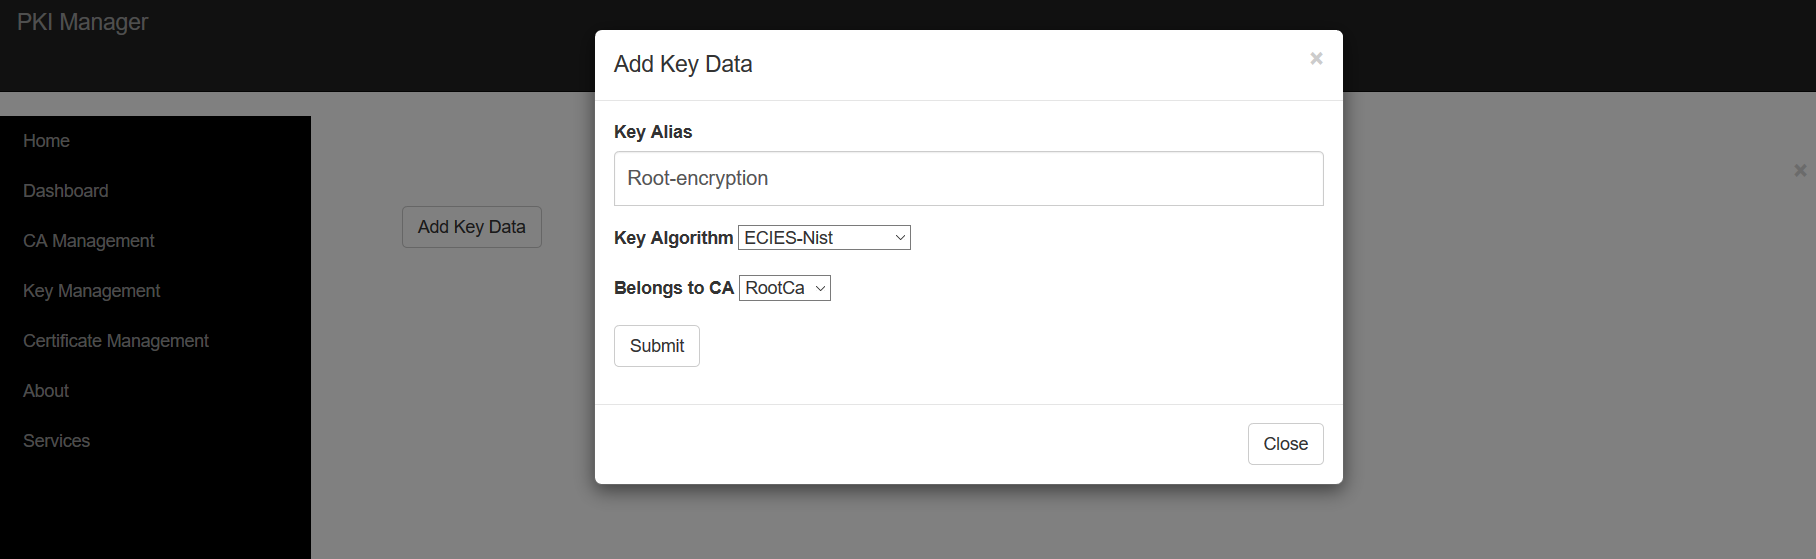
\includegraphics[width=0.8\textwidth]{Figures/manager3}
	\caption{\label{fig:manager3}Form to add a new keypair to an existing CA}
\end{figure}

\paragraph{Certificate Management}
The last step to have a functional CA is to generate its certificate. The Certificate Management page can be navigated to for this purpose. Once there, the user can generate a Root CA certificate or a Sub CA certificate by clicking the respective buttons. Generating a Root CA certificate involves filling the form shown in Figure \ref{fig:manager7} with the following information relative to the root certificate: time validity, country, and the Root CA which is the subject of the certificate. For the subject input the user is able to choose a CA from a list containing all the existing Root CAs which already have associated a signing keypair but no certificate. The list is provided by the server when the page is loaded and negates the user error of creating a certificate for a Root CA which is not ready to self-sign its certificate. Creating a Sub CA certificate is a very similar process with the difference that the user must fill the form displayed in Figure \ref{fig:manager8}. In this form the user must not only specify the subject of the certificate but also issuer CA. For the certificate's subject, a Sub CA with signature keys and no certificate must be selected. The issuer must be a Root CA which is ready to issue the certificate, i.e. a Root CA which has already has a signature keypair and a certificate associated. The mapping between a certificate and its issuer will allow the PKI Manager to build certification chains in the future. When the form is submitted, our server will compile the information inputted by the user, calling the V2X Library to issue the certificate and storing it on the database. Once these operations are finished, the server will refresh the Certificate Management page, updating the existing certificates table with the new entry. 

\begin{figure}
	\centering
	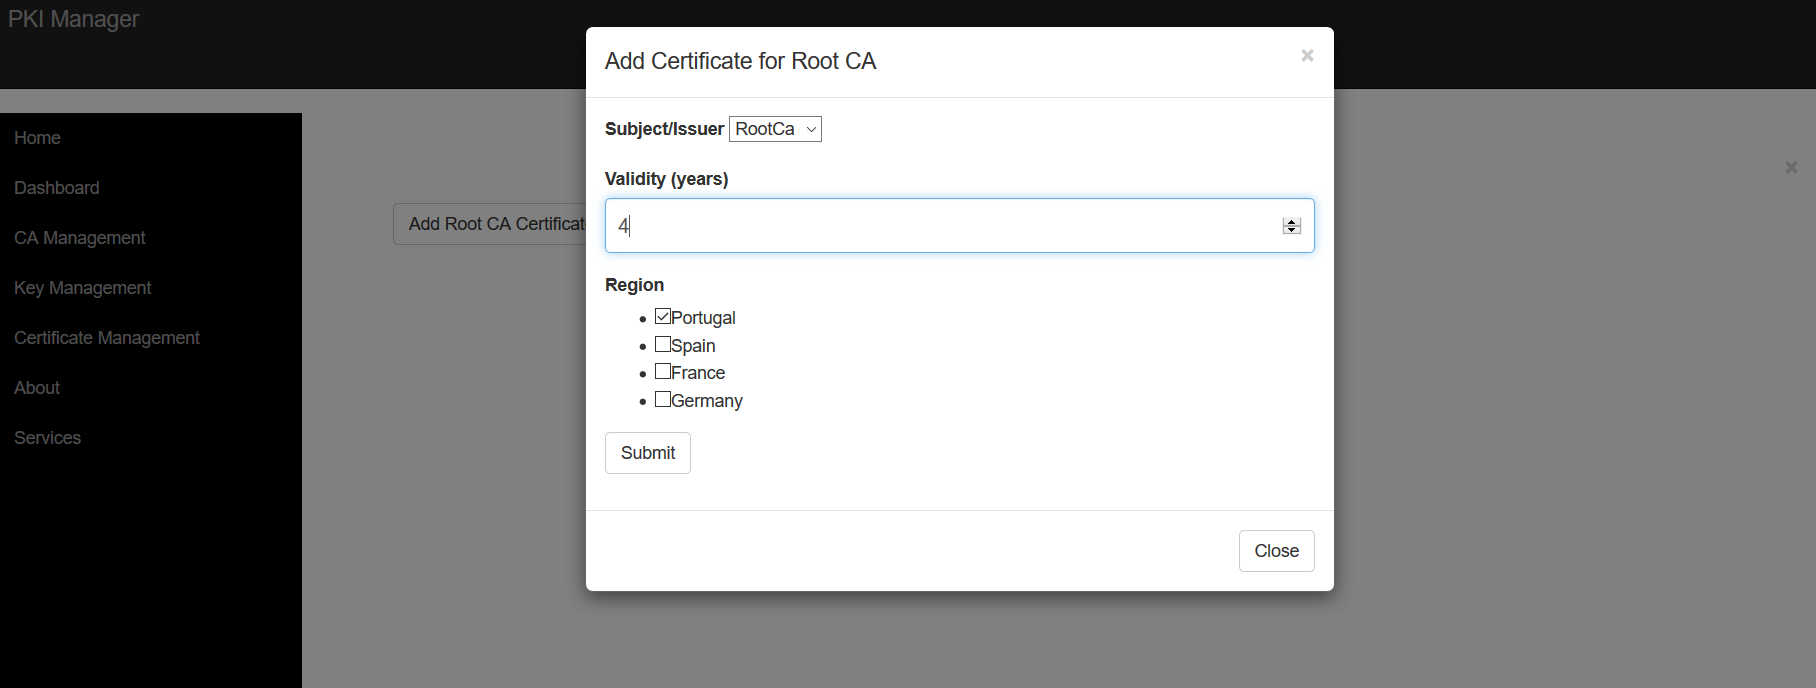
\includegraphics[width=0.8\textwidth]{Figures/manager7}
	\caption{\label{fig:manager7}Form to add a certificate to an existing Root CA}
\end{figure}

\begin{figure}
	\centering
	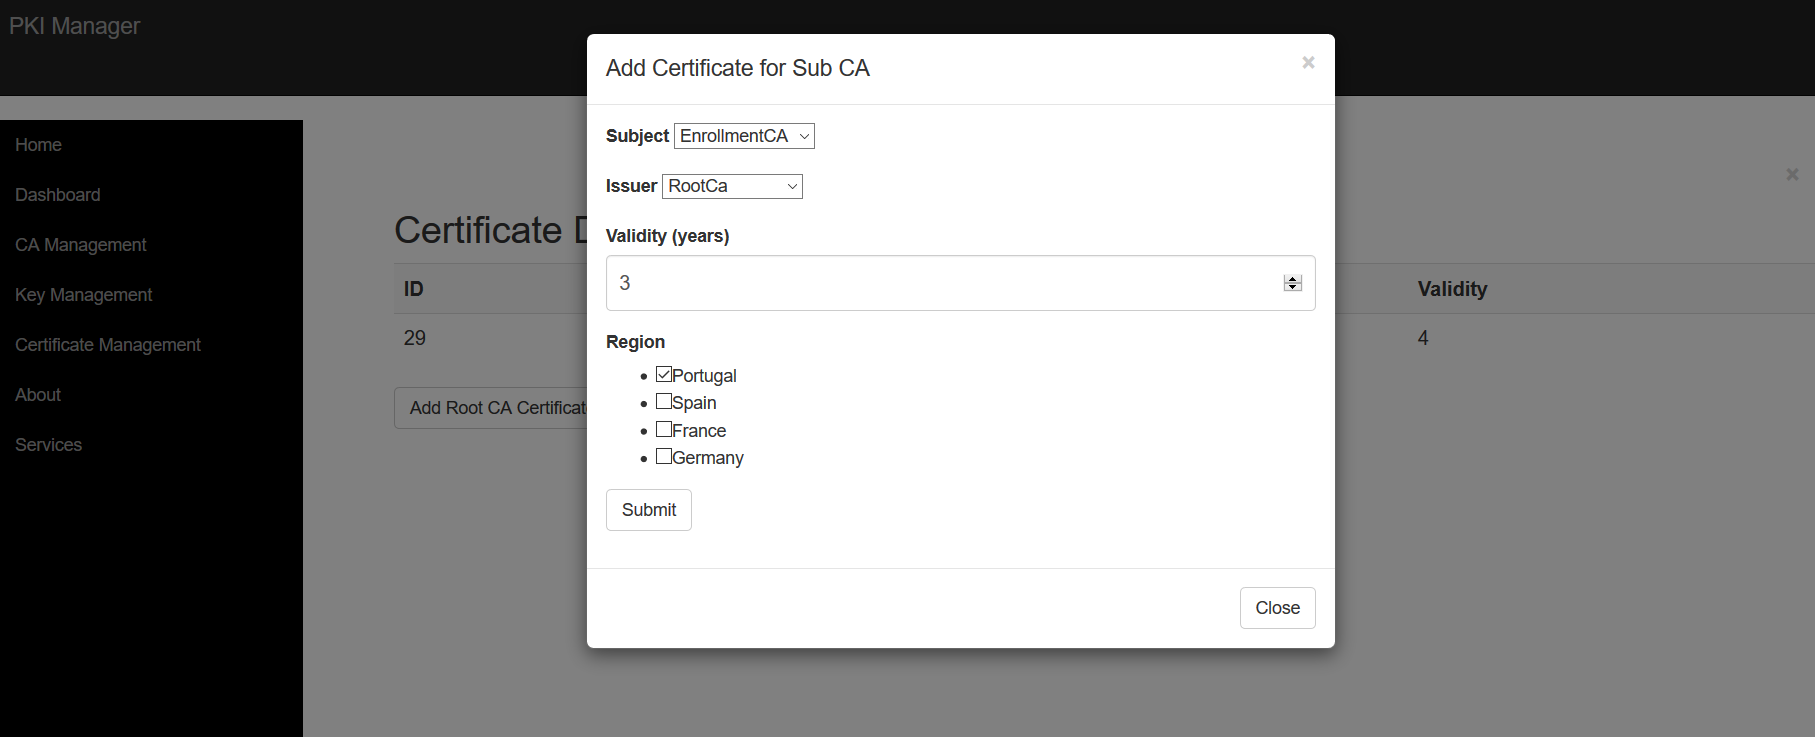
\includegraphics[width=0.8\textwidth]{Figures/manager8}
	\caption{\label{fig:manager8}Form to add a certificate to an existing Sub CA}
\end{figure}

\section{RA Service}
The RA Service can be seen as the gateway which allows vehicles to request certificates from the PKI. This gives the RA the responsibility of validating the origin of the requests, making sure that each vehicle is authentic, and also validating that the destination CA is ready to receive the request. In this section we discuss the implementation of the RA service, we start by describing the technologies then we take a look at the functionalities provided by the RA.

The RA service is a module of the PKI Manager, this means that it is implemented within the same Java project and thus shares the same resources, such as the database and the internal service layer. However, to give the illusion of distance between the RA and the PKI, we decided to separate the database into the part used by the PKI Manager and the part which is used by the RA. In addition, we also separated the internal services which the PKI provides to the RA from the services used by the PKI Manager to manage the PKI. At a high level, the RA Service is a RESTful API from which the PKI Manager is able to communicate over the internet with other software programs. 

A RESTful API is a set of end-points which any other application can communicate via HTTP protocol such as POST, GET, PUT, DELETE, etc. Such functions are defined in a special Spring MVC controller, each identified by an URL. In our case, we have an end-point for each service that the API exposes: vehicle configuration, enrollment, and authorization. Generally the data transferred between the client and such end-points (inside the HTTP requests) is objects from the common V2X library formatted using JSON. JSON is a human readable format for structuring and transmitting data objects, it relies on text key and value pairs. This implies that both the vehicle and server have a way of converting the original objects into a string based DTO \textit{data transfer object} and vice versa.

To document our API we decided to use the Swagger tool. From annotations on the source code, this tool is able to automatically generate an interactive API documentation which is accessible through the browser. In this documentation it is possible to understand: what operations do the API support, what are the parameters of each operation and the return values, if authorization is needed, and even usage licence information. This allows our API to be better understood by us, and any other client software that might want to communicate with the PKI manager. In the remainder of this section we describe the implementation of each operation provided by the RAService, for each operation we take a closer look at the request, end-point, and response.

\section{Vehicle Configuration}
The Vehicle Configuration is the first operation that should be requested by the new client vehicles. This service has two main functions: to configure the vehicle within the RA, and to provide an initial configuration within the vehicle regarding the PKI. The first function allows the RA to validate the identity of the vehicle on future interactions. The last aims to prepare the vehicle to request certificates, the goal is to simulate the PKI information that needs to be installed on the vehicle at manufacture time as specified in Section \ref{section:life-cycle}. In a real case scenario, the RA would not have this functions, as the configuration would be done in the vehicle and RA during the vehicle manufacture. However, for demonstration and testability purposes we decided to provide this service. 

\subsubsection{The request}
Figure \ref{fig:conf_req} illustrates the configuration request which the API is expecting to receive. In order to communicate with the API through the configuration end-point, a vehicle needs to be able to build such request. The canonical key is an encoded PublicVerificationKey structure as defined in our V2X library. The id represents the vehicle's unique name (ITS identifier). Finally, the type attribute represents a specific vehicle type, e.g. ambulance, truck, etc. To transfer this information the vehicle must compile such attributes into a string based DTO which is known by the server. Such object represents the request and contains each encoded in the String type. While the vehicle type and name are already string objects, the public key needs to be transformed in order to be a part of the request. Such transformation involves the vehicle encoding the \textit{PublicVerficationKey} using its \textit{encode} method, then transforming the outputted byte stream into a base64 String. 

\begin{figure}
	\centering
	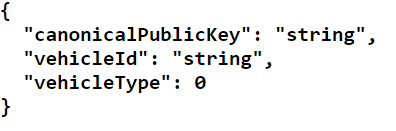
\includegraphics[width=0.5
	\textwidth]{Figures/conf_req}
	\caption{\label{fig:conf_req}Vehicle configuration request in JSON format.}
\end{figure}

\subsubsection{The end-point}
The RA service provides a POST controller dedicated to receiving the vehicle configuration requests. The first step that the RA does when it receives a configuration request is to try to save the vehicle's data in the database. However, it needs to first decode the JSON formatted data, because the request is a known DTO the RA knows how to decode it into its original objects. This is done by the \textit{DTOtoVehicle} method that exists on the RA's service layer, this method receives the request's \textit{VehicleDTO} and returns and object of \textit{Vehicle} which is a database entity containing each of the DTO's decoded attributes, and thus being more useful for the business logic. To achieve this, the \textit{DTOtoVehicle} method first decodes the base64 String canonical key to a steam of bytes and uses it to decode a \textit{PublicVerificationKey} object. The next step is to map the vehicle type to a vehicle profile name, a profile is built for a specific type of vehicle and contains generic vehicle information such as enrollment and authorization validity information. If these operations completed without generating exceptions and the requesting vehicle was not configured before, the vehicle configuration was successful and the\textit{DTOtoVehicle} method will return a new \textit{Vehicle} containing the vehicle's id, profile and canonical key, which will be stored in the RA's database under the \textit{vehicle} table as a new entry. 

\subsubsection{The response}
The next step is to respond to the vehicle with the PKI information. The response built by the RA is a \textit{ConfigResponse} DTO which always informs the vehicle of the response's origin, destination, and if the configuration was successful. Only in the positive case, the response will also contain the following PKI information: the certificate of the EA which will enrol the vehicle; the certificate of the AA that will authorize the vehicle; a list containing the certificates of all trusted AA which will allow the vehicle to trust incoming V2X messages; and the certificate of the Root CA which is the root of trust for this hierarchy. With this information the vehicle is able to request the RA for its enrollment certificate. 


\subsection{Vehicle Enrollment}
The vehicle enrollment operation can be used by configured vehicles to, as the name suggests, request a valid enrollment certificate. This operation involves the vehicle, the RA and the EA which is able to issue such certificate. During this communication, the RA has the function of assuring that the vehicle is configured and therefore authentic.

\subsubsection{The request}
Figure \ref{fig:enrol_req} illustrates the enrollment request which the API is expecting to receive. This DTO is composed of three elements: the destination representing the name of the EA which the vehicle is trying to contact, the encoded request which is an encoded \textit{EnrolmenRequest} as defined in Section \ref{requests}, finally the origin containing the vehicle's unique name (ITS identifier). For a vehicle to build the DTO which the RA is expecting to receive, it must be able to build and encode the \textit{EnrolmenRequest} element of the DTO as defined in the V2X Library. To do so, the vehicle first has to generate necessary cryptographic keys. Such keys are a new verification key pair, which the public key is to be certified by the enrollment certificate, and a symmetric AES key to encrypt the request and share with the EA. With these keys, the vehicle is able to use the V2X Library in order to generate and encode the \textit{EnrolmenRequest} data structure into a byte stream. The final step is to transform such byte stream into a base64 string and create the request DTO with the other origin and destination attributes.

\begin{figure}
	\centering
	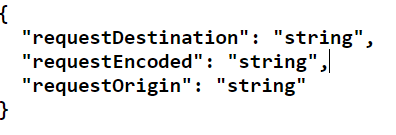
\includegraphics[width=0.5
	\textwidth]{Figures/enrol_req}
	\caption{\label{fig:enrol_req}Vehicle enrollment request in JSON format.}
\end{figure}

\subsubsection{The end-point}
The RA service provides a POST controller dedicated to receiving the vehicle enrollment requests. The first step that the RA does once it receives such request is try to verify its origin. This is done by the \text{verifySource} method which is implemented on the service layer of the RA. This method has two main functions, verifying that the vehicle is already configured within the RA, and if the destinations EA is ready to receive the vehicle's request. To do so, this method receives the request DTO as it was sent by the vehicle. First, it gets the origin of the request and queries the RA's database for that specific vehicle. In the event that the vehicle is not found, an appropriated exception will be thrown. Then using the name of the EA on the request's destination attribute, this method tries to find the such CA on the database. If found, it checks if the CA type is set to enrollment, it has signature and encryption keys, and a certificate associated. This is done to ensure that the EA that the vehicle is trying to contact is able to issue the enrollment credential. In the case that these verifications fails, an appropriate exception will be thrown. The last step is to try to decode the \textit{EnrolmenRequest} from its base64 string format into an array of bytes representing the V2X Library encoded data structure. 

Once the origin and destination of the request are verified by the RA, it is time to send the vehicle's request to the target EA. Since the PKI Manager and RA Service are part of the same project, this communication is achieved through a simple service call. The service layer of the PKI Manager provides the RA with the \textit{caService} class which contains every service which the CAs are able to provide. In this case the service needed by the RA is the \textit{validateEcRequest}, this method has the objective of validating the \textit{EnrollmentRequest} structure, therefore ultimately verifying the vehicle's identity. In order to do so, it needs to perform the following steps: decrypting the request, validating the vehicle's signatures within, and finally returning the \textit{EnrollmentResponse} which may contain the enrollment certificate. 

The RA calls the \textit{validateEcRequest} service by passing the \textit{EnrolmenRequest} and name of the EA, which were found on the vehicle's request DTO; and the vehicle's canonical key and profile name found on the RA's database under the vehicle's configuration information. In order to decrypt the request, this service first gets the stored information relative to the target EA. Using the name of the EA, it gets the EA's certificate from the PKI Manager database, and its encryption/signature key pairs from the \textit{KeyStore}. With the EA's relevant information, this service calls the V2X Library in order to decrypt the request. This is achieved through the V2X Interface which specifies the services available by the Library side to the PKI Manager. The \textit{decryptRequest} service given the encrypted \textit{EnrolmenRequest}, the EA's decryption key (private key) and certificate will verify if the request was encrypted to that EA, and if so decrypt it using the provided private key. To do so, it first decodes the byte encoded \textit{EnrolmenRequest} into an \textit{EncryptedData} structure, then using the cryptographic module of the V2X Library calculates the hash of the EA certificate and compares it to the hash that can be found within the recipient information field of the request. If there is a match, the symmetric encryption key will be decrypted using the private key of the EA, giving access to the key which encrypted the request. To decrypt the request, this method retrieves the AES cipher text field from the request and tries to decipher it using discovered symmetric key. In case that this method fails to perform such description operations or there is no match on the calculated EA certificate hash and recipient identifier within the request, an approprieate exception will be thrown by the service. Otherwise, the signed request will be returned containing the vehicle's signatures and the requested subject attributes.

The next step that the \textit{validateEcRequest} method does is to verify the vehicle's identity. To do this, it calls the \textit{verifyEcRequest} service provided by the V2X Library to verify the vehicle's signatures. This method uses the recently decrypted request and the vehicle's canonical public key to first verify the request's outer signature, this assures the EA that the vehicle that build the request has possession of the private canonical key which was attributes to it during manufacture. The next step is to verify the request's inner signature. To do so, the Library gets the inner signed structure from the request, from this structure extracts the verification public key which the vehicle is trying to get certified by the enrollment credential, and finally verifies the inner signature. This assures the EA that the vehicle has possession of the corresponding private key, therefore making it impossible for the EA to issue an enrollment credential to a vehicle which does not have the correct verification key pair. The verification of the enrollment request is only accepted if both signatures are valid. This service returns an enrollment response code which summarizes what happened during the request's validations, some possible outputs are: OK, can't parse, not the recipient, invalid signature, incomplete request, decryption failed, etc. 

\subsubsection{The response}
The final step is to build the response to the vehicle, this is done by the \textit{genEcResponse} service of the V2X Library which is called by the PKI Manager. Since it is at this step that the enrollment credential will be generated, the PKI Manager gets from its database the profile information of the vehicle using the profile name which was sent to it by the RA. This information is necessary to issue the enrollment credential as it contains information such as the default certificate time and geographic validity. The \textit{genEcResponse} service works with the signed request; the information of the EA, including its signature key pair and certificate; the vehicle's profile information; and the enrollment response code from the last step. The first verification done by this service is with the enrollment response code, if it is a negative code such as can't decrypt, invalid signature, can't parse, etc. A new \textit{EnrollmentResponse} \ref{requests} is built without the generation of the enrollment credential. If the response is OK, this service will issue the enrollment credential. This certificate is generated using the vehicle profile information and the inner enrollment request which contains the vehicle's verification key and requested subject attributes. Once the certificate is generated by the V2X Library, the \textit{EnrollmentResponse} is generated including the enrollment credential. In both cases, response is signed by the EA's signature key and encrypted using the shared symmetric key. Such response is returned to the PKI Manager which saves the credential on its database marked as active, identified by its hash, and issued by the specific EA. The final step is to return the encrypted response to the RA which sends it to the requesting vehicle. To do so, the RA first makes the \textit{EnrollmentResponse} object ready to be transferred by encoding it in base64 text and encapsulating in a response DTO. Then the RA's controller is able to return the vehicle's expected string based object. However, if the EA was not able to retrieve the shared symmetric key from within the \textit{EnrollmentRequest}, therefore it was not able to built the encrypted \textit{EnrollmentResponse}. In this case, the RA is notified and will send the response DTO marked as failed without the EA's response structure.


\subsection{Vehicle Authorization}
The vehicle authorization operation can be used by enrolled vehicles in order to request an authorization ticket. Such operation involves the vehicle, RA, EA, and the AA. As in the previous operations, the responsibility of the RA is to assure that the requesting vehicle is configured, and also decoding the string based request DTO so that they can be used by the PKI Manager's services.

\subsubsection{The request}
Figure \ref{fig:auth_req} illustrates the authorization request which the API is expecting to receive. This DTO is similar to the one expected by the enrollment end-point, the only differences are the encoded request which is an \textit{AuthorizationRequest} as defined in Section \ref{requests}, and the destination references the AA which will authorize the vehicle. To generate and encode such a request, the vehicle is able to use the V2X Library, it just needs to generate the necessary keys first. Such keys are a new verification key pair which will be certified by the authorization ticket, and two different symmetric keys in order to share with the EA and AA. Like the previous operations, the string based DTO forces the vehicle to be able to encode such \textit{AuthorizationRequest} in order to create the request which the RA is expecting.

\begin{figure}
	\centering
	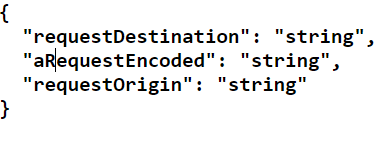
\includegraphics[width=0.5
	\textwidth]{Figures/auth_req}
	\caption{\label{fig:auth_req}Vehicle enrollment request in JSON format.}
\end{figure}

\subsubsection{The end-point}
The RA service provides a POST controller dedicated to receiving the vehicle authorization requests. The first step that the RA does once it receives such request is to try to verify its origin, this is done by the same \text{verifySource} method used in the enrollment operation. However, in the authorization operation the RA processes this step differently. As explained in the authorization protocol \ref{protocol}, the authorization process of a vehicle is composed of multiple individual authorization requests, each for an authorization ticket. Through this first step, the RA has the responsibility of determining if the received request is the first of the vehicles' authorization process or not. The \text{verifySource} method receives the request DTO as it was sent by the vehicle, after validating that the destination AA is ready to issue certificates it validates that the origin vehicle is configured in the RA. If the vehicle is found, then this method gets the maximum number of authorization requests that the vehicle is allowed to make from its profile information. Comparing this number to the number of requests done by this vehicle (identified by the origin on the request DTO) allows the RA to know if the received request is the first of the authorization process, and therefore if the vehicle's enrollment needs to be validated, see Figure \ref{fig:protocol_2}. To protect against vehicles using other vehicle's identifiers to request authorization tickets the SSL protocol is used. The communication security provided by the protocol allows to the RA to trust that the vehicles are in fact the ones that their secret identifier say they are. When a vehicle starts the authorization process it is expected by the RA that all the underlying requests will be done close to each other, in a sequence manner. However, if this is not the case it would be necessary to implement a cron based mechanism that after some time marks the vehicle so that the RA knows that its enrollment must be verified in the next authorization request regardless of the request counter. The last step done by this method is to try to decode the \textit{AuthorizationRequest} from its base64 string format into an V2X Library data structure. 


Once the RA has verified the origin, destination and determined the enrollment validation for the request, it is time to send the decoded request to the AA. To do so, the RA calls the \textit{validateAtRequest} on the CA's service layer. From all the services which the CA's are able to provide to the RA, this method can be seen as the service which the AA provides for the RA to send the vehicle authorization requests. Such method has the objective of validation the \textit{AuthorizationRequest} structure. To do so the following steps are performed: decrypting the request, validating the vehicle's signature, requesting the verification of the vehicle's enrollment if applicable, and finally generating the \textit{AuthorizationResponse} which may contained the issued authorization ticket.

The RA calls the \textit{validateAtRequest} by passing the \textit{AuthorizationRequest}, the name of the AA, the vehicle's profile name, and the flag that determines if the vehicle's enrollment is to be verified or not. The decryption of the request is similar to the process used by the vehicle enrollment operation: the \textit{validateAtRequest} service starts by getting the AA's certificate and keys from the database and \textit{KeyStore}. With this information it calls the same V2X Library \textit{decryptRequest} service which returns the signed request structure. With the decrypted request the AA is able to verify the vehicle's signature using the to be certified public verification key in the request. Such validation assures the AA that the vehicle which created the request has possession of the corresponding private key. In the eventuality that request is not valid because, for example, the request is badly formed, it was not encrypted to this AA, the signature is invalid, etc the response code to be delivered to the vehicle in the response will be of error.

\subsubsection{The response}
If the response code is positive and the enrollment validation flag was set to true by the RA in the last step, the next step is to request the EA for the validation of the vehicle's enrollment. This is done by first extracting the \textit{AuthorizationValidationRequest} structure from the now decrypted \textit{AuthorizationRequest}, the \textit{AuthorizationValidationRequest} structure contains the EA encrypted vehicle's enrollment signature and the shared request. The AA is able to find the hash of the EA's certificate within the shared request. With this information it is able to get the name of the EA from the database and send it the \textit{AuthorizationValidationRequest} by calling the \textit{validateEnrollment} CA service. In the case that the RA determined that the request is not to be enrollment verified, the call to the EA's \textit{validateEnrollment} service is skipped, 


The first step that this EA service performs is the decryption of the received request, to do so, it relies on the name of the EA to get its certificate and decryption key from the persistent layer of the PKI Manager. Once the decryption parameters are set, it calls the V2X library \textit{decryptRequest} service to decrypt the request. The next step is for the EA to validate the vehicle's enrollment by verifying its enrollment certificate and signature. First, this service gets the vehicle's credential from the database (stored by the EA at the enrollment phase) and checks if it is still marked as valid, if this is the case, then the service cryptographically validates the enrollment credential using the \textit{verifyCertificate} service provided by the V2X Library. This service, given a certificate and the corresponding certification chain will verify if such certificate belongs in that chain by decrypting its signature using the public verification key of the next certificate in the chain, in addition to this, it also validates the expiration date on the certificate. The return value is a simple boolean which, if true, allows the EA to continue with the vehicle's enrollment validation by decrypting its enrollment signature. This process can be started by calling the V2X Library \textit{verifyEnrollmentSignature} service which given the vehicle's enrollment credential and \textit{AuthorizationValidationRequest} is able to extract the enrollment signature from the request and verify it using the credential's public key. If the signature is valid the EA has validated the vehicle's enrollment and returns a positive response to the AA. In the case either the credential or the signature is not valid, a negative response will be sent yo the AA. 

The final step is to build the response to the vehicle which may contain the requested authorization ticket. To generate such response the AA, first gets its signature key pair; its certificate; the vehicle's profile information; the signed request; and the response code which resulted from the validation of such request and, if applicable, the vehicle's enrollment. With this information, the AA calls the \textit{genAtResponse} V2X service which is the response code is positive will issue the authorization ticket using the AA's certificate, private signature key and vehicle's profile information, including it in the response. The response structure is generated always signed by the AA and encrypted to the vehicle, (using the same symmetric key from the request). The final step is to return this response to the RA marked as positive so that it can be returned to the vehicle.


\section{Vehicle Manager}
The Vehicle Manager has the responsibility of generating client vehicles for the PKI Manager, at a high level we can see the Vehicle Manager as a vehicle manufacturer which is trusted by the RA service. In addition to generating the vehicles, it is this component's responsabilty to provide a V2X environment where the generated vehicles are able to communicate with each other. To ease the testability of such environment, the Vehicle Manager reads the application properties to load the execution variables, such as the number of vehicles, number of times a AT is used, pattern of certificate usage, etc.

At this point we have a REST API which is documented using the Swagger tool, Although the automatic and interactive documentation is useful in its own way, the main reason why we chose Swagger to document our the RA Service is the possibility of automatically generating client libraries for the API. For this purpose, we used the \textit{Swagger Codegen} tool, an open source project available on the \textit{GitHub} repository. This tool works with the URL of our API's documentation and is able to generate a client project where the communication layer is made to specifically communicate with the API. This allowed us to save time abstracting from the communication details and focus on the functionality of the Vehicle Manager.

The Vehicle Manager is a simple multi-threaded \textit{Java} project which can be started using the \textit{Main} method. The first operation done by the this method is to initialize the generation of vehicles, which is managed by other class. The output of the vehicle generator is a list containing the vehicles, each with a fixed size random \textit{String} as the identifier, and one of the V2X library supported encryption/signature algorithms. At this point the main method knows how many vehicles will participate in the execution so it populates each vehicle with a list of its neighbours. 

The multi-thread attribute of the Vehicle Manager comes into play right after the generation of the vehicles, where each vehicle represents a different thread in the execution of the application. Our objective with this is to make the V2X communications seem more realistic where each vehicle is sending messages to its peers in no particular order, resutling in different communication situations. 

The execution of the threads starts when the main method calls the \textit{start} method of the generated vehicles. When started, each vehicle performs the protocol described in Section \ref{protocol} by requesting the operations of the RA Service of vehicle configuration, enrollment and authorization. Using the V2X Library enables each vehicle to generate the most complext request elements. The result of the protocol is the installation of the CA certificates, the enrollment credential and a list of authorization tickets within each vehicle. 

Once a vehicle has all the needed certificates it is time to start communicating with its peers. To do so, it starts two timers: the \textit{CAMtimer} and the \text{includeCertTimer}. The first has the responsability of periodically sending CAMs, each time electing an authorization ticket to sign the message (currently used AT). The second timer informs the vehicle when it is time to send the full authorization ticket within the signer information of its next message so that it can be distributed. 

The process of broadcasting a CAM is composed of three steps: checking for unknown authorization tickets, generating the message, and sending it. In the first step the vehicle searches its internal list of unknown authorization tickets, if any hash is found then it will be included in the next CAM so that the corresponding full certificate can be requested. The generation of the CAM itself is done using the V2X Library with respect to the currently used AT, the corresponding signature keys, the list of unknown ATs, and wether to include the full signing AT or its hashed reference. Finally, in order to send the CAM the vehicle simply iterate through the list of neighbour vehicles calling their respective \textit{receiveCAM} method.
 
When a vehicle receives a CAM the first step is to look for the hash of its currently used AT within the list of requested certificates. If found, then the vehicle sets a variable to include its full AT on the next message. This mechanism allows the distribution of the currently used AT in the cases that other vehicles have requested it.
The next step is to try to verify the message. For this purpose, the vehicle first reads the message signer identifier in onder to understand the type of signature, i.e. if the message includes the signer's AT or the hash value. 

In the first case, the vehicle verifies the signer's AT against the certificates of the trusted authorization authorities. If the AT is signed by a trusted authorization authority, the vehicle stores it as trusted in a hash map enabling access on future communications, and proceeds to verify the message. This is a simple process where the signature is verified against the signer's AT, and the message generation time is within the certificate's expiration period.

In the case that the vehicle receives a CAM containing the hashed AT, the vehicle starts the verification of the message by looking for that digest on its trusted AT hashmap. If the hash is found it means that the AT was already verified and roots to a trusted AA certificate, so the message is able to be verified using the same method as in the previous case. However, if the AT is unknown the vehicle adds the digest to the list of unknown ATs so it can be requested in the next message. Because the message was not able to be verified due to the missing AT, it is stored in a list of pending messages which await verification until the full signing AT is included within an incoming CAM.

When a vehicle receives a CAM containing the full certificate it can be the consequence of this vehicle's request for an unknown certificate. Therefore, the vehicle tries to verify both the new and pending messages. For each pending CAM we compare the digest on the signer identifier to the digest of the received AT. A match means that the pending message was signed by that same AT, which if trusted by the vehicle, enabling the verification of the message.

\section{Summary}
In this chapter we presented our solution to the problem of implementing a PKI solution that allows a V2X environment while preserving the privacy of the vehicles. We started by overviewing the architecture of the solution, learning about its main components: PKI Manager, V2X Library and Vehicle Manager. We studied how such components are organized in a client-server architecture, assuming the PKI Manager as the server and the Vehicle Manager as the client. In addition, we seen that these two components communicate through the API of the server, the RA Service and utilize the V2X Library in order to generate the necessary messages. We concluded this chapter by presenting the detailed implementation of each component, where we also explained the technologies and external libraries adopted in order to implement our components. In the next chapter we perform an experimental evaluation to our V2X system, where we test the performance of the server, the resource usage of the client and finalize by discussing the security and privacy properties achieved. 

 
%%%%%%%%%%%%%%%%%%%%%%%%%%%%%%%%%%%%%%%%%%%%%%%%%%%%%%%%%%%%%%%%%%%%%%%%

\cleardoublepage

%%%%%%%%%%%%%%%%%%%%%%%%%%%%%%%%%%%%%%%%%%%%%%%%%%%%%%%%%%%%%%%%%%%%%%%%
%                                                                      %
%     File: Thesis_Implementation.tex                                  %
%     Tex Master: Thesis.tex                                           %
%                                                                      %
%     Author: Andre C. Marta                                           %
%     Last modified :  2 Jul 2015                                      %
%                                                                      %
%%%%%%%%%%%%%%%%%%%%%%%%%%%%%%%%%%%%%%%%%%%%%%%%%%%%%%%%%%%%%%%%%%%%%%%%






 % file "Thesis_Implementation.tex"
\cleardoublepage

%\input{Thesis_new_file} % add new .tex files for new chapters
% \cleardoublepage

%\input{Thesis_new_file} % add new .tex files for new chapters
% \cleardoublepage

%\input{Thesis_new_file} % add new .tex files for new chapters
% \cleardoublepage

%%%%%%%%%%%%%%%%%%%%%%%%%%%%%%%%%%%%%%%%%%%%%%%%%%%%%%%%%%%%%%%%%%%%%%%%
%                                                                      %
%     File: Thesis_Results.tex                                         %
%     Tex Master: Thesis.tex                                           %
%                                                                      %
%     Author: Andre C. Marta                                           %
%     Last modified :  2 Jul 2015                                      %
%                                                                      %
%%%%%%%%%%%%%%%%%%%%%%%%%%%%%%%%%%%%%%%%%%%%%%%%%%%%%%%%%%%%%%%%%%%%%%%%
\chapter{Evaluation}
\label{chapter:results}

This chapter describes the evaluation of our V2X system, which comprises the PKI Manager and Vehicle Manager. The three main non-functional requirements of our V2X system are performance, security, and privacy. With this in mind, we intend to answer the following questions: 

\begin{enumerate}
	\item Since interoperability is a constant concern, does the system provide acceptable performance? 
	\item Does the system deliver the necessary conditions for vehicle privacy, authentication and overall security?
	\item Does the implemented V2X environment provide vehicle privacy at an acceptable cost?
\end{enumerate}


The following sections address these three questions, staring with the performance and resource usage tests, moving to the privacy and security concerns. 

%%%%%%%%%%%%%%%%%%%%%%%%%%%%%%%%%%%%%%%%%%%%%%%%%%%%%%%%%%%%%%%%%%%%%%%%
\section{Performance}
\label{section:performance}
Performance is a fundamental concern when testing systems that address a sensitive subject such as road safety. The most common metrics of performance are latency and throughput: latency is the time necessary to complete certain operations and throughput in our case is defined by the number of requests that the PKI Manager processes in a determined time frame. While latency gives us an idea on how fast users are able to use each service, throughput relates to the capacity of the PKI Manager to process multiple requests in a given amount of time.

Such two performance metrics correspond to the metrics measured by our tests to the PKI Manager at different variants. To perform this evaluation several tests were done regarding the backoffice application, and the interaction between the Vehicle Manager and PKI Manager. The environment in which they execute is the following: 

\begin{itemize}
	\item A single installation of the PKI Manager application as the server. 
	\item A basic but functional vehicular PKI including one Root CA, one Enrollment CA, and one Authorization CA.
	\item A single installation of the Vehicle Manager application as the client. 	
\end{itemize}
Our goal with this setup is to provide a simple but complete V2X environment, where we can use the installation of the PKI Manager to test the performance of the backoffice and RA Service, and use the Vehicle Manager to execute tests focused the resource usage of V2X communications. 

\subsection{PKI Manager}
The PKI Manager is the component of our system which comprises the web application. Therefore, the performance tests done to the PKI Manager have the main goal of understanding how the application behaves under different work load conditions. These tests focus on two aspects: latency measurements of the operations supported by the backoffice application, and the latency resulting from the communications between client vehicles and the PKI through the RA Service operations.

Because the PKI Manager tests involve client-server communication over the network, we executed them on two different machines connected through the same network. The server ran on an Asus laptop with 16GB of RAM and an i7 Intel CPU. For the backoffice testes, the URL was accessed on the browser of the second machine and the measurements were taken using the network tab on the browser's developers console. Regarding the tests to the RA Service, the client vehicles were generated on the second machine using \textit{Apache Jmeter} \cite{jmeter}, an open source software designed for testing the performance of web applications. This configuration allows us in both test suits to consider the latency introduced by the network communications and the latency of the processing time at the server. 


\subsubsection{Backoffice Application}
The operations performed by the administrator application are simple but essential in order to have a functional PKI to serve as the backbone of trust within V2X communications. The processing is mostly located at the V2X Library, creating a waiting period in the backoffice application. On the administrator side, it makes sense to only test the latency of the operations performed by one user only, as this application is not meant to be used by many users concurrently. Next, we take a look over the operations evaluated on the backoffice: the generation of keys and certificates. 

The operation to add a key involves the following steps: generating a cryptographic key using the V2X Library, then storing it on a keystore and its information on the database. The operation to add a certificate is more complex than the previous, as it also involves searching for the keys which will be relevant to issue the certificate. Because of this factor, we included on the add certificate test the number of keys that exist on the system to provide a comparing factor amongst the different latency times. For each operation the timer started when the form was submitted (POST) and stopped when the page finished loading (GET). The reasoning behind not considering the generation of CAs in the test suit comes from the fact that, unlike the tested operations, generating a CA consists only in creating a simple database object and storing it. 


In Table \ref{tab:table1} we can observe the time necessary to complete the operations involving our backoffice application, which preclude user interaction. Overall from the perspective of an administrator the results are reasonable and will not negatively affect the usability of the application. Regarding the operation to add a certificate, the operations for adding a single key or certificate are fast, taking on average 71.6 and 73.7 milliseconds. There is a linear relation between the time that the system takes to add a certificate and the number of keys that exist on storage. This happens due to the nature of the operation, in which the server has to query the database and the keystore in order to find the cryptographic keys of the subject and issuer before calling the V2X Library to issue the certificate, and finally storing it on the database. This increase in delay is not critical, as considering a realistic number of keys (i.e., in the order of a few dozen keys) it does not affect the user experience to a point that it is noticeable.

\begin{table}
	\renewcommand{\arraystretch}{1.2} % more space between rows
	\centering
	\begin{tabular}{lccc}
		\toprule
		Operation           & $Time$ & $Keys$& $StandardDeviation$ $$\\
		\midrule
		Add key          & 71.6ms & 1 & 14.0ms   \\
		Add certificate  & 73.7ms &4& 10.0ms     \\
		Add certificate  & 81.0ms &20& 13.5ms     \\
		Add certificate  & 103.0ms &30& 14.0ms     \\
		Add certificate  & 128.6ms &40& 16.0ms     \\
		Add certificate  & 178.7ms &60& 19.5ms \\
		\bottomrule
		\end{tabular}
		
		\caption{Time needed to add a certificate and a key, calculated over twenty measurements.}
		\label{tab:table1}
	\end{table}
	
	\subsubsection{RA Service}
	
	The RA Service API is the gateway from which the vehicles are able to interact with the PKI to request certificates. Comparing with the backoffice application, the operations done by the RA Service are more complex and subject to more load due to the possibility of concurrent requests from the client vehicles. Therefore, the tests done to this component are designed to evaluate the behaviour of the API at different levels of server load. Ideally, to ensure that the results are as close to the reality as possible, API load tests are run on a production or equivalent system. However, in our case this was not possible so the results may differ depending on the machine which they run. In the remaining part of this section we take a look at the performance tests performed to the RA Service starting with latency of the supported operations moving to the throughput measurements. 
	
	\paragraph{Latency}
	
	Figure \ref{fig:graphs2} shows the tests done to the RA Service: latency resulting from the configuration, enrollment and authorization of vehicles respectively. As discussed before, we used \textit{Jmeter} in order to test each end-point. This tool allowed us to configure different number of users or virtual threads and send concurrent requests to the server automatically. For each operation we performed a total of 50 tests across different thresholds of concurrent users. We started with one user, tested 10 times, then increasing the number of users in order to increase the load on the server and provide a comparing factor between the latency times. The plot for each operation relates the number of concurrent users to the time needed to perform the operation. The time is the average of 10 measurements, where each test was performed when the previous was done processing. For each test, \textit{Jmeter} started the timer when the POST request was submitted by the thread and stopped it once the response was received. Meaning that the processing time done at the client side to build the requests and verify the responses is not included in our test results. All three operations involve reading the database, and the V2X Library to decode the request and build a response. In addition to this, both the enrollment and authorization of vehicles use the library to validate the vehicle's request and issue the certificate. For the authorization end-point we tested both use cases, as represented by Figure \ref{fig:protocol_2}: the authorization process without the enrollment verification (c), and the full authorization process (d).
	
	\begin{figure}
		\begin{subfigmatrix}{2}
			\subfigure[Vehicle Configuration]{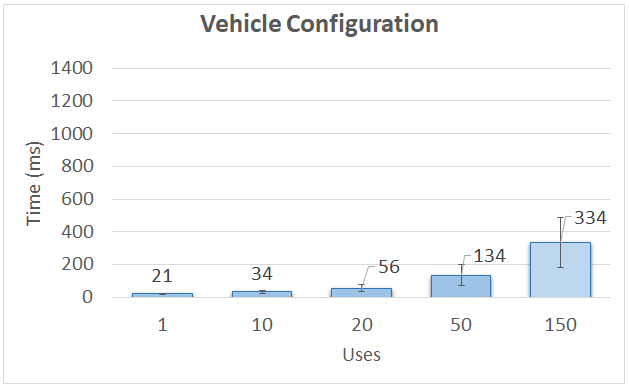
\includegraphics[width=0.49\linewidth]{Figures/conf_graph2.png}}
			\subfigure[Vehicle Enrollment]{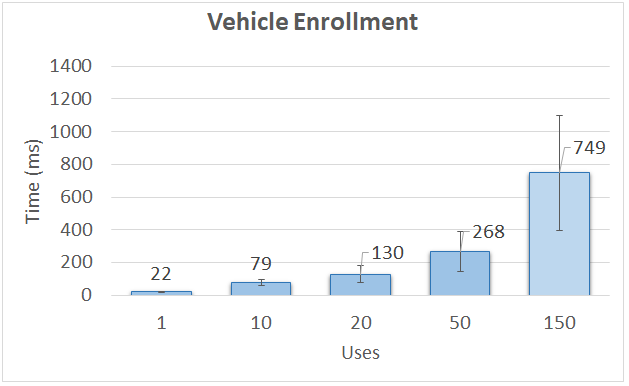
\includegraphics[width=0.49\linewidth]{Figures/enrol_graph2.png}}
			\subfigure[Vehicle Authorization w/o enrollment validation]{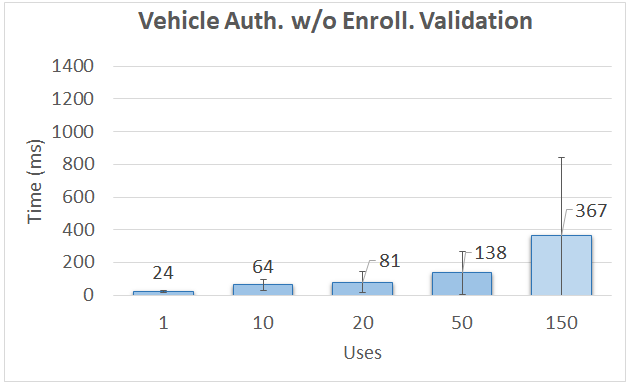
\includegraphics[width=0.49\linewidth]{Figures/new_auth_graph2.png}}
			\subfigure[Vehicle Authorization]{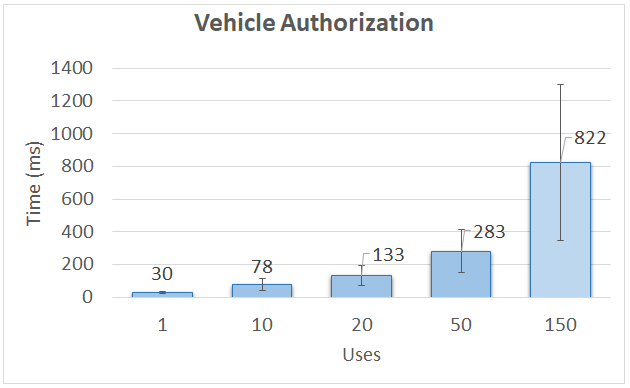
\includegraphics[width=0.49\linewidth]{Figures/auth_graph2.png}}
		\end{subfigmatrix}
		\caption{Latency measurements for the RA Service operations}
		\label{fig:graphs2}
	\end{figure}
	
	
	
	As we can see from the plot (d), the authorization of vehicles while verifying their enrollment is the operation which overall introduces more latency, with values varying from 30ms to 822ms. This happens due to the fact this operation is the most complex in terms of computation. Specifically, in the request validation where this version of the vehicle authorization requires the validation of two signatures: the signature that proves the possession of the verification keypair, and the vehicle's enrollment signature. In addition to this, the vehicle's enrollment credential is also verified.
	
	The second most expensive operation is the enrollment of vehicles (b) with latency values ranging between 22ms and 749ms. Comparing to the previous operation the enrollment of vehicles is simpler. The main difference comes from the validation of the vehicle's request, which in this case only requires the validation of two signatures: the canonical signature and the proof of possession signature. However, as we can see from plots (b) and (d) for all numbers of users the enrollment operation introduces almost as much latency as the more complex authorization, with values between 30ms and 822ms. This is because, unlike the previous operation, the enrollment of vehicles also requires saving on the database each enrollment credential issued, which introduces a bottleneck on the enrollment operation.
	
	Perhaps the most interesting comparison allowed by these tests is the comparison of the latency introduced by the two different vehicle authorization methods. As we can see from plots (c) and (d), the authorization without vehicle configuration introduced by our RA Service is on average faster than the standard full authorization flow. For example, considering the lowest server load of 1 user the new authorization flow represents an improvement of 16.6\% of the full authorization. As the number of concurrent users increases so does the improvement reaching its maximum value on the 150 user threshold with an improvement of 55.7\%. Since this version of the authorization is the most frequently used throughout the authorization process of the vehicles, the performance gains mean that the efforts presented in Section \ref{protocol} to optimize the authorization process as a whole were successful from a performance point of view. 
	
	The configuration of vehicles (a), being the simplest operation, introduced the least latency reaching a maximum of 334ms. Unlike the previous operations, the configuration of vehicles does not require signature validation at the application level or issuing certificates. It mainly requires decoding the request from the vehicle and read/writes to the database. However, the configuration of vehicles shares the same problem as the enrollment operation as the number of concurrent requests increases, i.e., database inserts become more and more expensive. At a 150 user mark it becomes almost as slow as the authorization of vehicles w/o enrollment validation (c), which is an operation that in terms of business logic is more complex. 
	
	One way to solve the problem shared by the configuration and enrollment operations is to increase the scalability of the data access layer by effectively managing the database writes. This can be achieved by using batch calls instead of single insert calls. Since we are using the default single insert calls, the number of writes results in same number of SQL \textit{insert} operations, which in turn result in that equal number of database round rips. Batching is a mechanism capable of grouping the \textit{inserts}, reducing the database round trips, and consequently increasing the performance of the data access layer. 
	
	\paragraph{Throughput}
	
	To test the throughput of the PKI Manager we used \textit{Jmeter} to generate requests to the vehicle authorization end-point since it is the most complex operation. This tool allowed us to configure five tests each with different ramp-up times. Each test was configured to 600 threads (users). The ramp-up period for each test was 60, 40, 30, 10 and 5 seconds respectively. Ramp-up period indicates the time duration that \textit{Jmeter} takes to start all the threads for that test. For example, if the ramp-up time is 10 seconds in a test with 10 threads it means that each thread will start after (10/10) 1 second. Having this mechanism in mind we reduced the ramp-up time in each test while maintaining the same number of users to increase of concurrency and work load on the server, providing a comparing factor between the resulting throughput measurements. It is important to note that, as explained in the documentation of \textit{Jmeter} \cite{throughput}, the throughput is calculated as (number of requests) / (total time) where time is calculated from the start of the first thread to the end of the last. For our tests the number of requests is constantly 600 and the total time is the period which took the test to fully execute. Specifically, starting with the first request (thread 1) and ending when the response to the last request is received (thread 600).
	
	Table \ref{tab:table2} relates the throughput measurements for each test done to the authorization of vehicles. In this table we can see the average latency of the 600 requests, the standard deviation of the latency, the throughput value, the percentage of failed requests and the test execution time. As we can see from the results, for the first three tests the server responded very well to the increase in the work load. We can see in the first test that for a ramp-up time of 60s the throughput was 10 requests per second. As the test was running for approximately 60 seconds, we can conclude that all the 600 requests were completed in approximately the same time as the ramp-up period meaning that the server was not delaying requests. This factor along with the low average request latency of 29ms, low standard deviation of 7.2ms and request error rate of 0\% allows us to conclude that this test was not able to reach the full capacity of the server. Therefore, the throughput was not higher because of the high ramp-up time that took to create the 600 requests. The same trend was maintained for two more tests, in the test with 30s ramp-up we can see that for twice the initial work load, the server responded with double throughput of 20 requests per second. This, along with the request latency still being low and no request errors is a further indicator the server was not yet saturated.
	
	However, once we increase the load by setting the ramp-up time to 10s the average latency of the requests started to increase to 592ms, which resulted in a higher standard deviation of 496.6ms as some requests were being processed fast while other were being delayed. For this test the throughput of the server was 52.8 request per second meaning that it was no longer increasing linearly in function to the increase in the work load. This is a sign that we are closer to reaching the server's capacity. Despite this, the average latency is still acceptable and because the error rate is 0 \% this test qualifies as a good performance output. As expected in the next test where we set the ramp-up to 5s, corresponding to twice the load as in the previous test, the throughput while still high (62.5/sec) increased at a lower rate comparing to the last 4 tests. The high average request latency of 2659ms and 12\% error rate on the requests is an indicator that we reached the full capacity of the server and for this work load it does not provide good performance.
	
	\begin{table}
		\renewcommand{\arraystretch}{1.2} % more space between rows
		\centering
		\begin{tabular}{lccccc}
			\toprule
			Ramp-up           & $Latency$& $Latency Standard Deviation$ & $throughput$& $TestTime$ $$\\
			\midrule
			60s          & 29ms & 7.2ms & 10.0/sec & ~60s  \\
			40s          & 28ms & 5.9ms & 14.9/sec & ~40s  \\
			30s          & 34ms & 5.6ms & 20.0/sec & ~30s \\
			10s          & 592ms & 496.6ms & 52.8/sec & ~11s \\
			5s           & 2659ms & 1480.6ms & 62.5/sec & ~9s \\
			\bottomrule
			\end{tabular}
			
			\caption{Throughput measurements to the authorize vehicle operation with 600 threads.}
			\label{tab:table2}
		\end{table}
		
		
		
		\subsection{Vehicle Manager}
		\label{section:memory}
		At the Vehicle Manager level, the focus of the latency/throughput metrics tests shifts from performance to resource usage. This is because the performance of the V2X communications could not be accurately measured by only using the Vehicle Manager. In the previous cases where the performance of the web application was tested we were able to relate the number of users to the latency needed to complete certain operations, which gave a general idea of how the system reacts under different work loads. This is not the case with the Vehicle Manager. The time needed to send messages from one vehicle to another (represented by objects within the Vehicle Manager) depends entirely on the system where the application is running. Without access to vehicle specialized V2X hardware the time taken by our testbed computer to generate, send and validate V2X messages is not conclusive. In addition to this, the network latency resulting from sending messages could not be accurately simulated because the communications within the Vehicle Manager's vehicles are represented by simple method calls. 
		
		In order to have a general notion of the possible quantities and the necessary storage capacity, Table \ref{tab:table3} lists the type of certificates, their size, and possible quantity. As described in Section \ref{etsi_design} all vehicles have to store different certificates on their local system. To estimate the size of the different certificates we used the \textit{java.lang.instrumentation} package \cite{instrumentation}, where we measured size of the ASN.1 COER encoded certificates (i.e. encoded using the V2X Library methods). Regarding the possible quantity of ATs stored within the vehicles, the values are estimated considering the AT usage pattern presented in Section \ref{section:at_usage}, assuming that a vehicle uses on average five certificates per day with a refill time of one year. In terms of numbers, the expected AT number can be calculated as (5 certificates) * (365 days) which equals to 1825 ATs. For the number of CA certificates we assumed a decently sized truststore installed on the vehicle. As we can see from Table \ref{tab:table3}, the authorization tickets and their corresponding private keys are the elements which demand more storage space (413.4KB), corresponding to approximately 87\% of total. It is also important to note that the number of the certificates can change from vehicle to vehicle depending on the usage pattern and the desired level of privacy, so the overall certificate storage demand may not be the same for different types of vehicles. This is further discussed in the following section.
		
		\begin{table}
			\renewcommand{\arraystretch}{1.2} % more space between rows
			\centering
			\begin{tabular}{lccc}
				\toprule
				Certificate & $Size$ & $Quantity$& $TotalSize$ \\
				\midrule
				Root CA         & 272 bytes & 20 &5.3KB \\
				Enrollment CA  & 288 bytes &100&28.1KB \\
				Authorization CA  & 288 bytes&100&28.1KB\\
				Enrollment Credential  & 208 bytes &1 & 0.2 KB\\
				Authorization Ticket  & 200 bytes &1825 & 356.4KB\\
				AT private key & 32 bytes & 1825 & 57.0KB\\
				\midrule
				\null  & \null & \null & 475.1KB\\
				\bottomrule
			\end{tabular}
			
			\caption{Estimated vehicle certificate storage demand}
			\label{tab:table3}
		\end{table} 
		
		\section{Security}
		\label{section:pricacy}
		In this section we analyse how our system achieves the security goals previously defined in Section \ref{goals}. In particular, we discuss the following security properties: confidentiality, data authenticity, and authorization.
		
		\subsection{Confidentiality}
		Confidentiality over the communications in an important characteristic of our system. Given that it falls outside the scope of V2X communications to restrict access to messages to certain users, the confidentiality aspect of our system only applies to the communication between the Vehicle Manager and PKI Manager.
		
		To ensure confidentiality, all the information transmitted from and to the client is sent through an SSL secure channel. In this communication channel the Vehicle Manager is authenticated, where the server requires its certificate in order to accept communications. 
		
		In addition, we also provide application level encryption where every certificate request is encrypted by the vehicle so that only the intended recipient CA is able to decrypt it. This feature combined with the encryption of the response to the original vehicle allows the confidentiality of the vehicle's identity, preventing its disclosure during the certificate requests.
		
		\subsection{Data Authenticity}
		Data authenticity enables the receiver of a message to confirm the origin and integrity of the data. In our system, this property applies to both the client-server communication and V2X messages.
		
		Regarding the Vehicle to PKI communication, the authenticity of the messages is achieved at two levels: first at the channel and then at the application levels. The sender of messages is the Vehicle Manager and the recipient is the PKI Manager. When the vehicles are manufactured, the RA trusts the new connections because of the SSL connection with the Vehicle Manager, which can be seen as the vehicle manufacturer. However, after the configuration of such vehicles the authenticity of their certificate requests is achieved at the application level, through the use of digital signatures.
		
		The authenticity of the V2X messages is a similar process where a vehicle being the recipient of a V2X message is able to trust the authenticity of the message by verifying the signature of the sender vehicle against a trusted certificate chain. 
		
		\subsection{Authorization and Authentication}
		Authorization over services requires user authentication. In our system this is applied in two aspects: the authentication of the administrator to manage the PKI and the client vehicles to request certificates. 
		
		The authentication of the administrator is accomplished through the use of a username/password mechanism, where the credentials are stored within the database of the server. Specifically, the password is hashed with the \textit{Bcrypt} algorithm before being saved to avoid mainlining it in clear text. The implementation of the hashing function is provided by \textit{Spring Security} and is prepared to internally generate and maintain a random salt value to be hashed alongside the password.
		
		The access to the data stored within the database is protected by username/password authentication. In addition to this, the access privileges are different depending on the type of user accessing it.
		
		Regarding the authorization of the vehicles, this is achieved through the RA service of vehicle configuration. Only vehicles which completed this service are recognized by our server and are able to request certificates.
		
		
		\section{Privacy}
		In our system preserving the privacy of users is one of the most important concerns. Losing privacy might mean that an attacker is able to track vehicles using the V2X communications, which is undesired. The main system variables that might affect the privacy of its users are the number of pseudonym certificates, and the usage pattern. The more pseudonym certificates a vehicle has available, the better is the privacy because the vehicle will have more choices when changing pseudonym. However, as described in the previous sections the increase of privacy comes with the overhead of the increase in certificate storage demand, number of individual certificate requests, and consequently processing at the vehicle. In this section we analyze different V2X scenarios, where we relate a vehicle's movement pattern, the pseudonym usage, possible types of attackers and the resulting level of privacy.
		
		\subsection{V2X Scenarios}		
		Regarding the types of vehicle trips, we wanted to choose real life cases where V2X communications could be involved. For the privacy scenarios we considered the following cases:
		\begin{itemize}
			\item \textbf{Vehicle A:} Round trip, the typical daily home to work commute.
			\item \textbf{Vehicle B:} One-way Trip, from point A to B.
		\end{itemize}
		
		
		The usage of certificates to sign V2X messages introduces privacy concerns over the communication. Therefore, the pattern which vehicles use pseudonyms and the frequency in which the certificate are changed are very impactful variables. We considered the following pattens:
		\begin{itemize}
			\item \textbf{Pattern A:} The vehicle always uses different pseudonyms.
			\item \textbf{Pattern B:} For a period of time the vehicle uses all the available pseudonyms then, if necessary, reuses the certificates in a different order.
		\end{itemize}
		
		To represent a challenge to the system's privacy, we choose different types of attackers differentiated by their power to capture messages within an area of operation.
		\begin{itemize}
			\item \textbf{Attacker A:} Controls a single section on the road while being able to visualize the victim vehicle and capture all messages.
			\item \textbf{Attacker B:} Controls two distant sections on the road where the victim vehicle will pass.
			\item \textbf{Attacker C:} Attacker is moving for a limited period following the victim vehicle. 
		\end{itemize}
		
		
		
		\subsection{Privacy Levels}
		
		Table \ref{tab:table3} organizes the scenarios from the lowest possible privacy to the highest.
		
		\begin{table}
			\renewcommand{\arraystretch}{1.2} % more space between rows
			\centering
			\begin{tabular}{lccc}
				\toprule
				Vehicle Type           & $CertificatePattern$& $VulnerableToAttacker$ &$PrivacyLevel$ $$\\
				\midrule
				A      & B      & A,B,C & Low\\
				B      & B      & B,C & Medium\\
				A      & A      & C & High\\
				B      & A      & C & High \\
				\bottomrule
				\end{tabular}
				
				\caption{Privacy scenarios ordered by level of privacy.}
				\label{tab:table3}
			\end{table}
			
			\subsubsection{Low Privacy}		
			Starting with the least privacy, vehicles of type A (round trips), using and reusing certificates as in th pattern B with low pseudonym change (e.g. using the same certificate for hours) are vulnerable to all types of attackers. Considering the attacker A there is a window of vulnerability if the vehicle passes the area controlled by the attacker twice with the same pseudonym. In this case the attacker is able to map that pseudonym to the victim's vehicle. Eventually, when the vehicle reuses the compromised pseudonym it may be possible for the attacker, if capturing the messages, to infer the vehicle's route. The same situation happens when considering the attacker B but with a bigger window of opportunity as the vehicle passes the areas controlled by the attacker twice as more. Because the frequency of certificate change is low it directly affects the privacy of the vehicle when considering the attacker C. In this case, the longer the vehicle uses the same certificate the bigger the probability of the attacker seeing that constant message broadcast by the vehicle, therefore mapping the used pseudonym to the identity of the vehicle and enabling short-term tracking. Despite the fact that this pseudonym usage pattern is worst in terms of privacy for the vehicles usually commuting, it is the least expensive in terms of certificate storage demand because the vehicle is reusing certificates with a low change frequency. 
			
			A privacy improvement for the same conditions (Vehicle type A, and certificate pattern B) would be to increase the frequency in which the vehicle changes pseudonyms. In this case, the vehicle would be more protected against the three types of attackers. In the case of attacker A and B, this is achieved because it would reduce the risk of the vehicle still be using the same certificate while passing through the zone(s) controlled by the attacker. The increase in privacy against attacker C is based on the unlinkability attribute of the pseudonym certificates. This means that when a vehicle changes pseudonym the new certificate can not be mapped to the old, therefore reducing the ability of the attacker to infer which certificate belongs to the vehicle. However, in order to assure the unlinkability of the pseudonym certificates care must be taken regarding the aggregation of information written on the certificate. For example, if a set of the vehicle's certificates have the exact same expiration date an attacker could infer that they belong to the same vehicle, disrupting the unlikability of the affected certificates. 
			
			\subsubsection{Medium Privacy}
			Medium privacy is achieved for vehicles of type B (one-way trips) using the certificate pattern B. In this case the vehicle can expect an improvement in the privacy level because it does not pass the same road twice. This is particularly effective when considering attackers of type A and B which control fixed areas of such road. For the first type of attacker, it is only possible to map a certificate to the vehicle if the vehicle passes the controlled area twice on different trips using the same certificate. Regarding the attacker B, it is possible to compromise a certificate if the vehicles passes the two controlled areas using the same certificate. As in the previous case, increasing the certificate change frequency will further decrease the power of the three attacker to compromise certificates for when the vehicle reuses them.
			
			
			\subsubsection{High Privacy}
			The best privacy for all vehicle types is achieved through the usage the certificate pattern A. Because certificates are not reused, even if the attacker manages to map a pseudonym to the victim's vehicle it is only possible to track the vehicle for the duration that it uses that certificate (short-term tracking). Increasing the certificate change frequency will further reduce the power of the attacker. 
			
			
			
			\subsection{Discussion}
			A general rule of thumb that is important to consider when using pseudonyms is that a pseudonym is only effective in a crowd. In vehicular communications this means that a pseudonym certificate is only effective if there are more vehicles around using them. If a vehicle is isolated on a road sending V2X messages signed with a pseudonym certificate then that certificate can be immediately mapped to the sender, even considering a high pseudonym change frequency.
			
			We have seen in the scenarios presented above that pseudonyms are particularly vulnerable to reuse attacks where the attacker is able to map a specific certificate to a vehicle. In this case the pseudonym becomes compromised because the attacker will be able to link that certificate to the vehicle when it reuses it. The more certificates are compromised the bigger the chance of the attacker to infer a vehicle's route by observing the compromised certificates being reused at different locations. However, assuming that vehicles carry thousands of pseudonyms, a few compromised certificates might not be conclusive for the attacker. It all depends on the power of the attacker to compromise certificates by controlling areas and/or following the victim vehicle, the number of certificates reused by the vehicle, and the randomness in which they are selected. 
			
			We also have seen that having a low pseudonym change frequency is particularly vulnerable to short-term tracking attacks where the attacker is following the vehicle and is able to: (a) see the vehicle using the certificate while isolated, or (b) infer it by the captured messages which are signed constantly by the same certificate. We concluded that the best way to preserve privacy is to increase the number of pseudonyms, which enables the possibility of a higher pseudonym change frequency and lowers the need to reuse certificates. 
			
			More concretely, the price in terms of storage in order to have acceptable privacy depends on the travel distance of the vehicles. In the previous section, we estimated that if a vehicle uses on average 5 pseudonyms in a day with a refill time of one year it would need approximately 486.6KB of certificate storage space. Depending on the distance that a vehicle travels each day, it may need to use more that 5 certificates resulting in the reusage of certificates, and privacy loss in most cases. To assure that this does not happen a vehicle that spends more time on the road needs more certificates. For example, assuming a vehicle changes certificate each 10 minutes and an average travel time of 2 hours each day. The vehicle would need approximately 12 certificates a day in a total of 4380 for a year. Assuming the same number of PKI certificates as in the previous section \ref{section:memory}, this number of pseudonyms would increase the storage demand to approximately 1MB.
			
			
			\section{Sumary}
			In this chapter we presented the evaluation results of the developed V2X system. We started by evaluating the performance of the PKI Manager, then looked at the resource usage of the Vehicle Manager and finished by discussing the security properties and privacy of the system.
			
			The performance of the PKI Manager was measured at two different variants: the backoffice application and the RA Service. In the evaluation of the backoffice we measured the latency of the most complex PKI operations, the generation of keys and CA certificates. We concluded from the results that the measurements were reasonable, considering the complexity of the operations, and would not negatively affect the usability of the application by an administrator. From the results it was possible to conclude that the most expensive operations in terms of latency are the full authorization and enrollment of vehicles. The new authorization of vehicles introduced by our RA Service was faster than the standard full process. 
			
			Lastly we presented how our system provides the security properties of confidentiality, data authenticity and authorization in both vehicle to PKI and V2X Communications. We concluded this chapter by analyzing how the privacy of the vehicles is maintained in V2X communications, discussing the different levels of privacy achieved by different vehicle types and pseudonym usage patterns.
			
			%%%%%%%%%%%%%%%%%%%%%%%%%%%%%%%%%%%%%%%%%%%%%%%%%%%%%%%%%%%%%%%%%%%%%%%%
 % file "Thesis_Results.tex"
\cleardoublepage

%%%%%%%%%%%%%%%%%%%%%%%%%%%%%%%%%%%%%%%%%%%%%%%%%%%%%%%%%%%%%%%%%%%%%%%%
%                                                                      %
%     File: Thesis_Conclusions.tex                                     %
%     Tex Master: Thesis.tex                                           %
%                                                                      %
%     Author: Andre C. Marta                                           %
%     Last modified :  2 Jul 2015                                      %
%                                                                      %
%%%%%%%%%%%%%%%%%%%%%%%%%%%%%%%%%%%%%%%%%%%%%%%%%%%%%%%%%%%%%%%%%%%%%%%%

\chapter{Conclusions}
\label{chapter:conclusions}

Insert your chapter material here...


% ----------------------------------------------------------------------
\section{Achievements}
\label{section:achievements}

The major achievements of the present work...


% ----------------------------------------------------------------------
\section{Future Work}
\label{section:future}

A few ideas for future work...

 % file "Thesis_Conclusions.tex"
\cleardoublepage

% ----------------------------------------------------------------------
%  Bibliography
% ----------------------------------------------------------------------

% Add entry in the table of contents as chapter
\phantomsection
\addcontentsline{toc}{chapter}{\bibname}

% Include all references in .bib file, even non-cited ones...
%\nocite{*} % this should be used carefully because it is not correct!

% Produces the bibliography section when processed by BibTeX
%
% Bibliography style
% > entries ordered alphabetically
%\bibliographystyle{plain}
% > unsorted with entries appearing in the order in which the citations appear.
%\bibliographystyle{unsrt}
% > entries ordered alphabetically, with first names and names of journals and months abbreviated
%\bibliographystyle{abbrv}
% > entries ordered alphabetically, with reference markers based on authors' initials and publication year
%\bibliographystyle{alpha}
%
% Replacement bibliography styles provided by 'natbib' package
% (plainnat.bst, abbrvnat.bst, unsrtnat.bst )
% > entries ordered alphabetically
%\bibliographystyle{plainnat}
% > unsorted with entries appearing in the order in which the citations appear.
%\bibliographystyle{unsrtnat}
% > entries ordered alphabetically, with first names and names of journals and months abbreviated
%\bibliographystyle{abbrvnat} % <<<<< SELECT IF USING REFERENCES BY AUTHOR/YEAR
% > entries ordered alphabetically, with reference markers based on authors' initials and publication year
%\bibliographystyle{alpha}
%
% Custom bibliography style adapted from 'natbib' package
%   (based on http://tex.stackexchange.com/questions/5053/is-it-possible-to-get-unsrt-abbrv-bibliography)
%   (unsrtnat.bst + abbrvnat.bst -> abbrvunsrtnat.bst)
%   (original files copied from:
%   http://tug.ctan.org/macros/latex/contrib/natbib/abbrvnat.bst
%   http://tug.ctan.org/macros/latex/contrib/natbib/unsrtnat.bst
% > unsorted with entries appearing in the order in which the citations appear, with first names and names of journals and months abbreviated.
\bibliographystyle{abbrvunsrtnat} % <<<<< SELECT IF USING REFERENCES BY NUMBER (CITATION ORDER)

% External bibliography database file in the BibTeX format
\bibliography{Thesis_bib_DB} % file "Thesis_bib_DB.bib"

\cleardoublepage


% ----------------------------------------------------------------------
\end{document}
% ----------------------------------------------------------------------

